\documentclass[9pt]{article}
\usepackage[english]{babel}
\usepackage{amsmath,amsthm}
\usepackage{amsfonts}
\usepackage{graphicx}
\usepackage[margin=0.2in]{geometry}
\newcommand{\setlinespacing}[1]{\setlength{\baselineskip}{#1 \defbaselineskip}}
\newcommand{\doublespacing}{\setlength{\baselineskip}{2.0 \defbaselineskip}}
\newcommand{\singlespacing}{\setlength{\baselineskip}{\defbaselineskip}}
\newcommand{\A}{{\cal A}}
\newcommand{\h}{{\cal H}}
\newcommand{\s}{{\cal S}}
\newcommand{\W}{{\cal W}}
\newcommand{\BH}{\mathbf B(\cal H)}
\newcommand{\KH}{\cal  K(\cal H)}
\newcommand{\Real}{\mathbb R}
\newcommand{\Complex}{\mathbb C}
\newcommand{\Field}{\mathbb F}
\newcommand{\RPlus}{[0,\infty)}
\newcommand{\norm}[1]{\left\Vert#1\right\Vert}
\newcommand{\essnorm}[1]{\norm{#1}_{\text{\rm\normalshape ess}}}
\newcommand{\abs}[1]{\left\vert#1\right\vert}
\newcommand{\set}[1]{\left\{#1\right\}}
\newcommand{\seq}[1]{\left<#1\right>}
\newcommand{\eps}{\varepsilon}
\newcommand{\To}{\longrightarrow}
\newcommand{\RE}{\operatorname{Re}}
\newcommand{\IM}{\operatorname{Im}}
\newcommand{\Poly}{{\cal{P}}(E)}
\newcommand{\EssD}{{\cal{D}}}
\newcommand{\field}[1]{\mathbb{#1}}
\newcommand{\C}{\field{C}}
\newcommand{\R}{\field{R}}
\newcommand{\script}[1]{\mathcal{#1}}
\newcommand{\fall}{\; \forall \;}
\newcommand{\exts}{\; \exists \;}
\newcommand{\mbf}[1]{\mathbf{#1}}
\newcommand{\binomial}[2]{\biggl( \begin{array}{c}  #1 \\ #2  \\ \end{array} \biggr) }
\newcommand{\fderiv}[2]{ \frac{d}{ d #1} \: #2}
\newcommand{\sderiv}[2]{ \frac{d^2}{ d^2 #1} \: #2}
\newcommand{\pfderiv}[2]{ \frac{\partial}{ \partial #1} \: #2}
\newcommand{\psderiv}[2]{ \frac{\partial^2}{ \partial^2 #1} \: #2}
\newcommand{\mat}[1]{\mathbf{#1}}
\DeclareSymbolFont{AMSb}{U}{msb}{m}{n}
\DeclareMathSymbol{\dblz}{\mathalpha}{AMSb}{"5A}
\DeclareMathSymbol{\dblr}{\mathalpha}{AMSb}{"52}
\DeclareMathSymbol{\dblt}{\mathalpha}{AMSb}{"54}
\DeclareMathSymbol{\dblq}{\mathalpha}{AMSb}{"51}
\DeclareMathSymbol{\dbln}{\mathalpha}{AMSb}{"4E}
\DeclareMathSymbol{\dblf}{\mathalpha}{AMSb}{"46}
\DeclareMathSymbol{\dblc}{\mathalpha}{AMSb}{"43}
\DeclareMathSymbol{\dbld}{\mathalpha}{AMSb}{"44}
\theoremstyle{plain}
\newtheorem{thm}{Theorem}[section]
\newtheorem{cor}[thm]{Corollary}
\newtheorem{lem}[thm]{Lemma}
\newtheorem{prop}[thm]{Proposition}
\theoremstyle{definition}
\newtheorem{defn}{Definition}[section]
\theoremstyle{remark}
\newtheorem{rem}{Remark}[section]
\numberwithin{equation}{section}
\renewcommand{\theequation}{\thesection.\arabic{equation}}
\begin{document}
\title{Regression of KL Software Distribution   }
\author{KL Software Libraries}
\date{Sat Jul 12 09:01:22 2014
}
\maketitle
\textbf{ KL Library test output.  This LaTex file and the associated diagrams are produced by the KL software libraries.}
\subsubsection{Matrix Quick Check <double>}
QueryPerformanceCounter  =  2.4622
\subsubsection{ARPACK versus Lapack SYEVX}
Running Arnoldi Krylov algorithm on affinity matrix and comparing to Lapack SYEVX (via Intel MKL).
tic toc fileistream read dim n=512 dt=1.65095
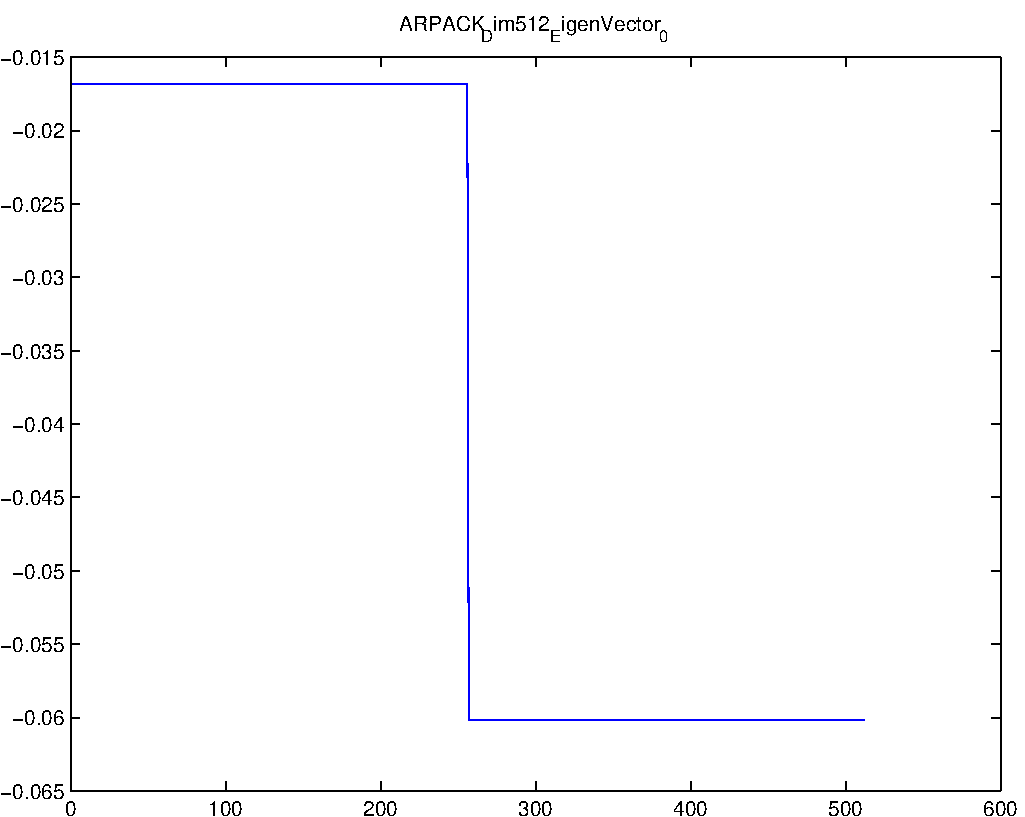
\includegraphics[width=10.0cm,height=10.0cm]{ARPACK_Dim512_EigenVector_0.pdf}

\includegraphics[width=10.0cm,height=10.0cm]{ARPACK_Dim512_EigenVector_1.pdf}

\includegraphics[width=10.0cm,height=10.0cm]{ARPACK_Dim512_EigenVector_2.pdf}

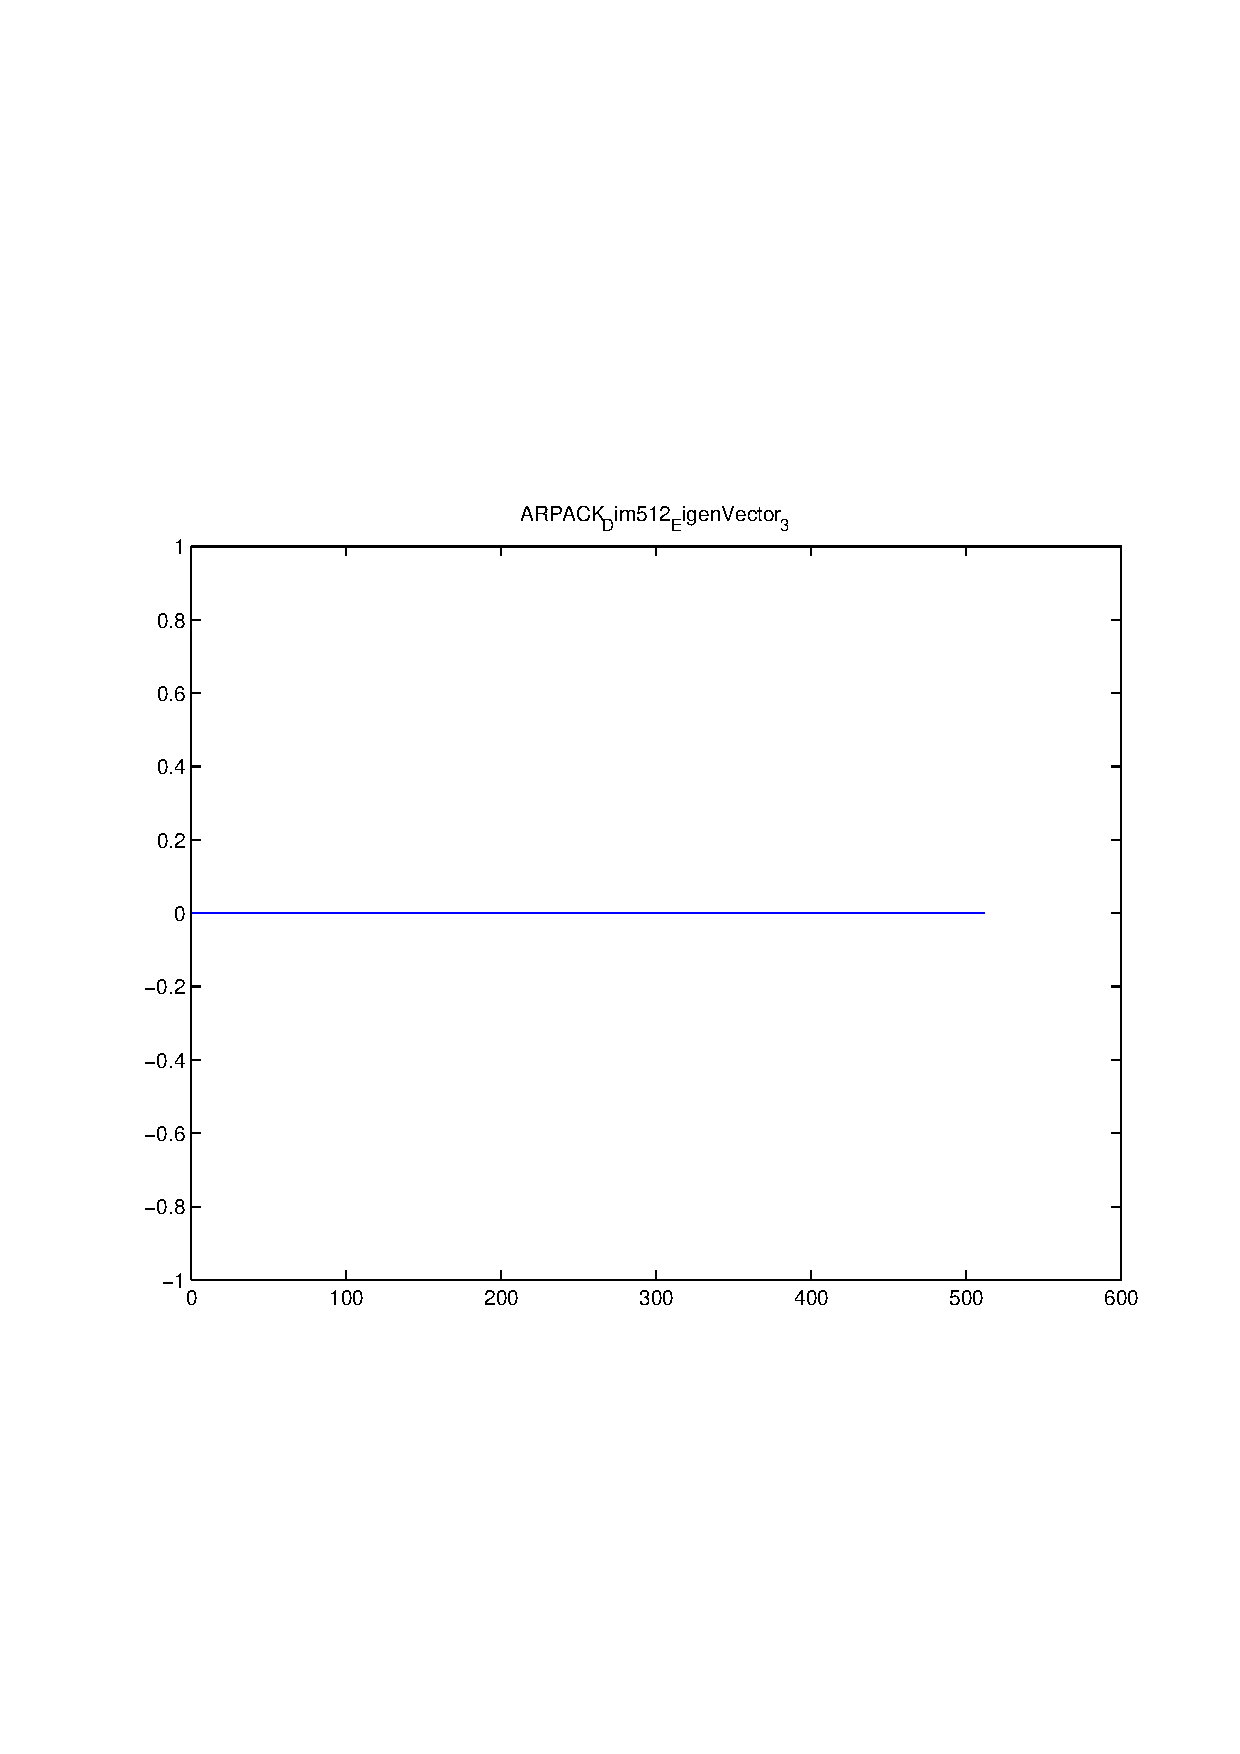
\includegraphics[width=10.0cm,height=10.0cm]{ARPACK_Dim512_EigenVector_3.pdf}

\includegraphics[width=10.0cm,height=10.0cm]{ARPACK_Dim512_EigenVector_4.pdf}

Iterative Krylov dim=512 dt=9.55056
\includegraphics[width=10.0cm,height=10.0cm]{SYEVX_Dim512_EigenVector_1.pdf}

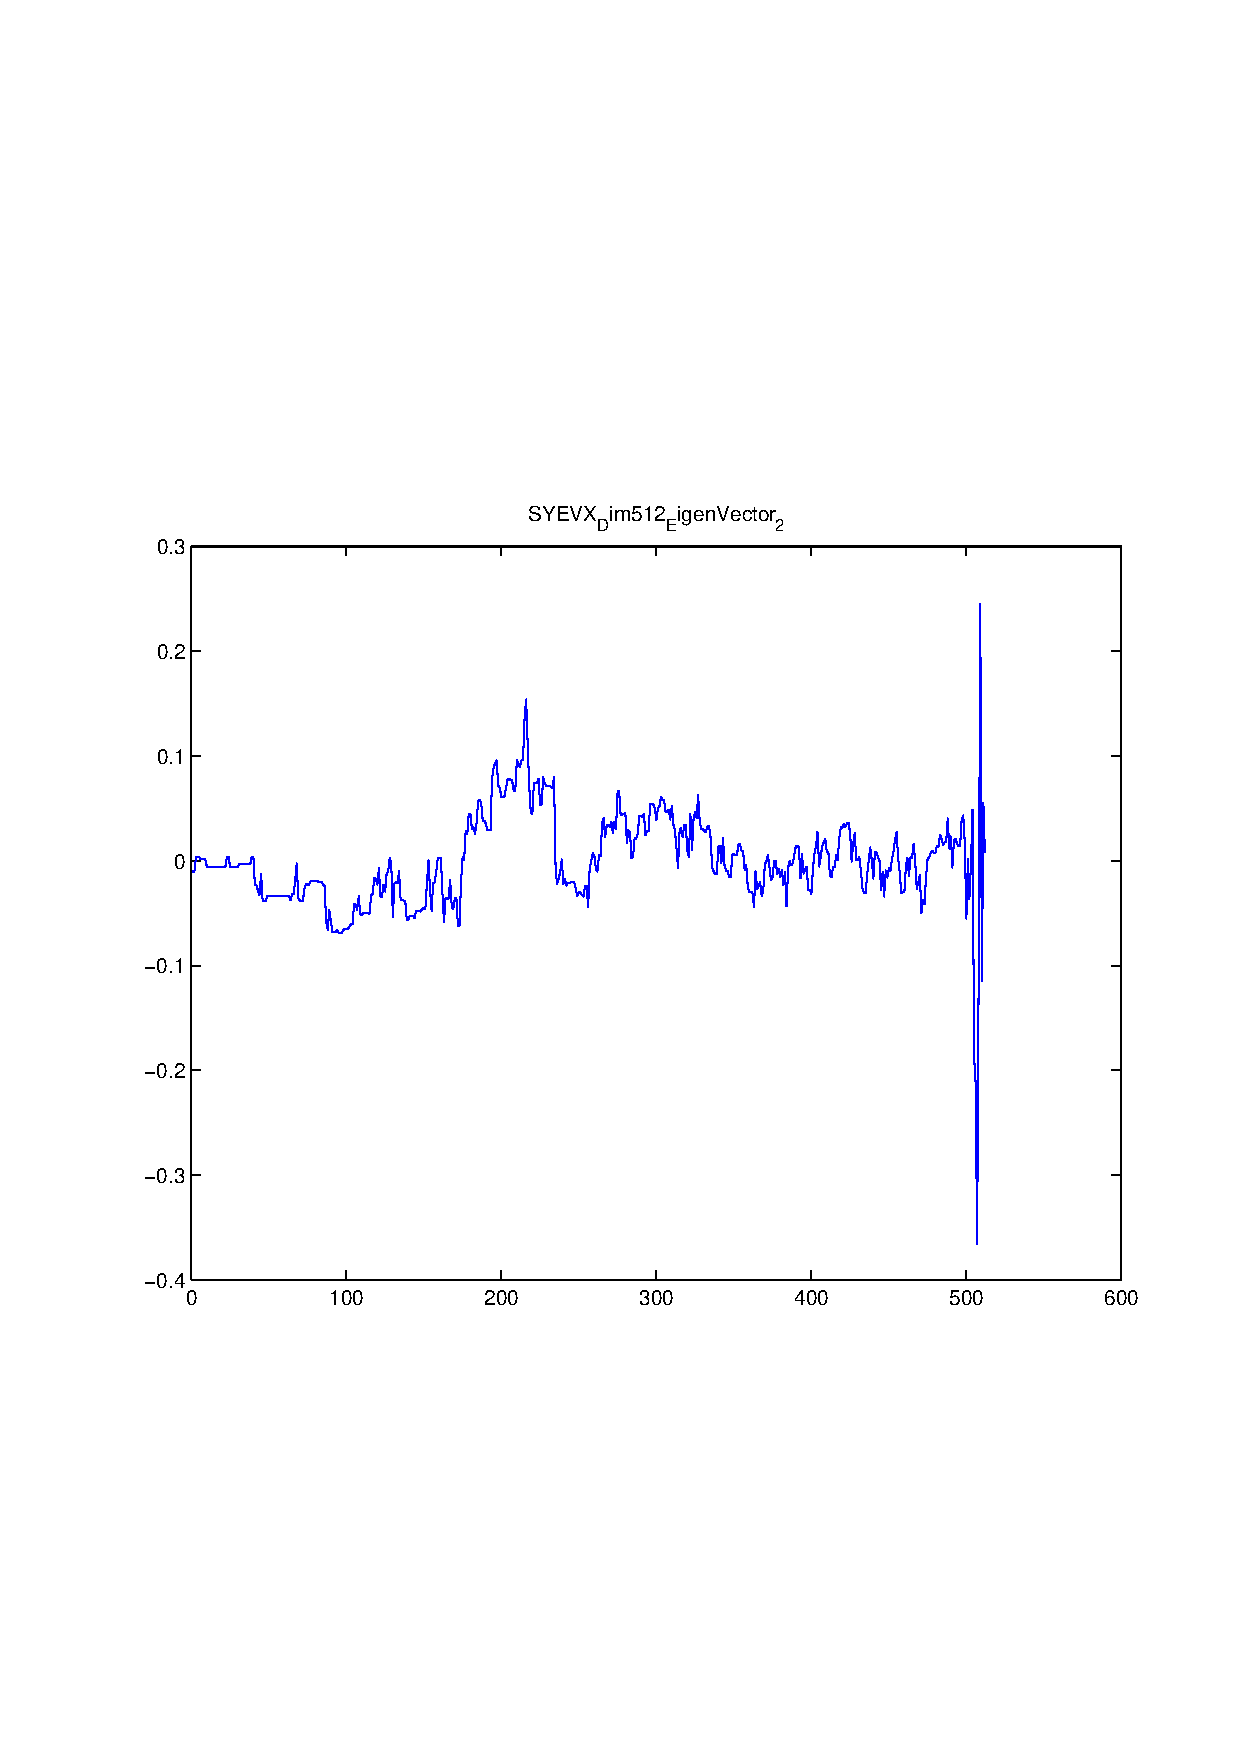
\includegraphics[width=10.0cm,height=10.0cm]{SYEVX_Dim512_EigenVector_2.pdf}

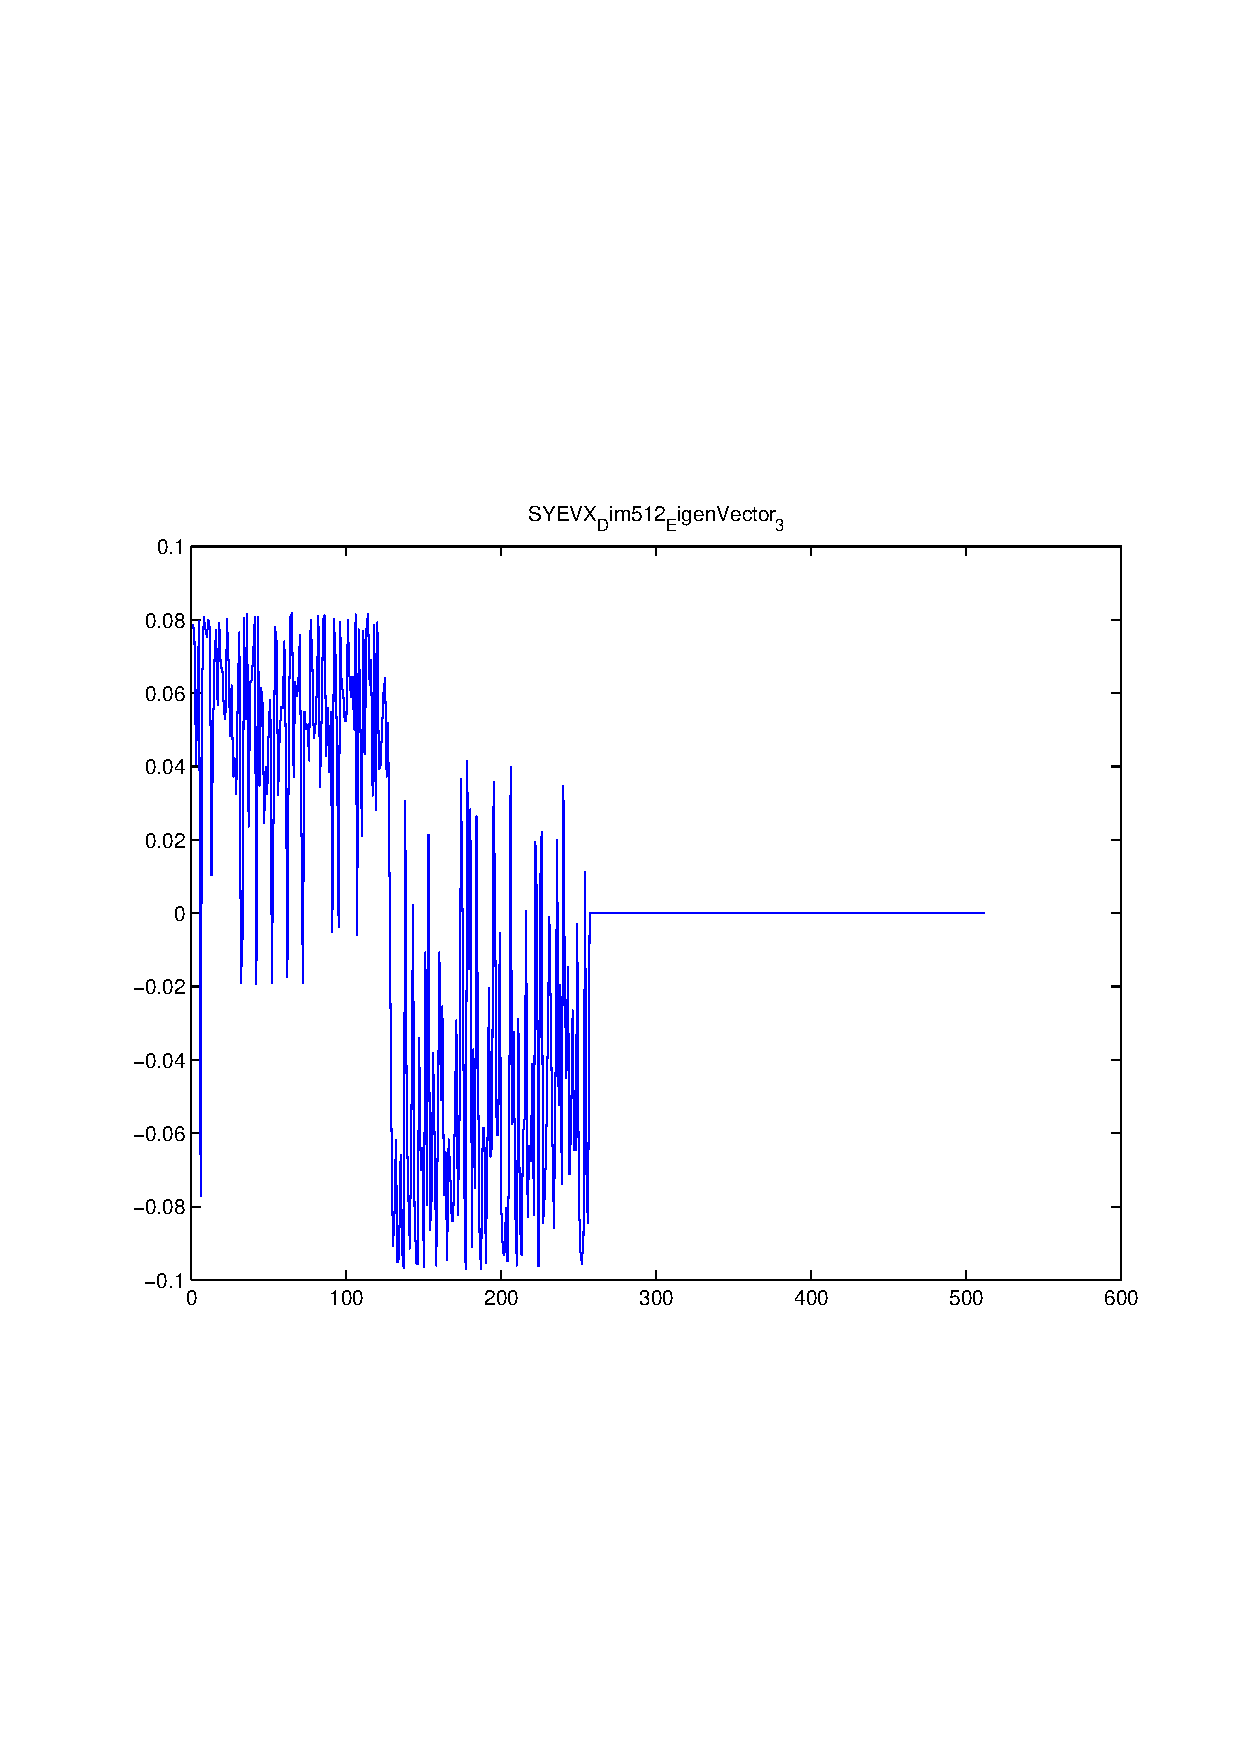
\includegraphics[width=10.0cm,height=10.0cm]{SYEVX_Dim512_EigenVector_3.pdf}

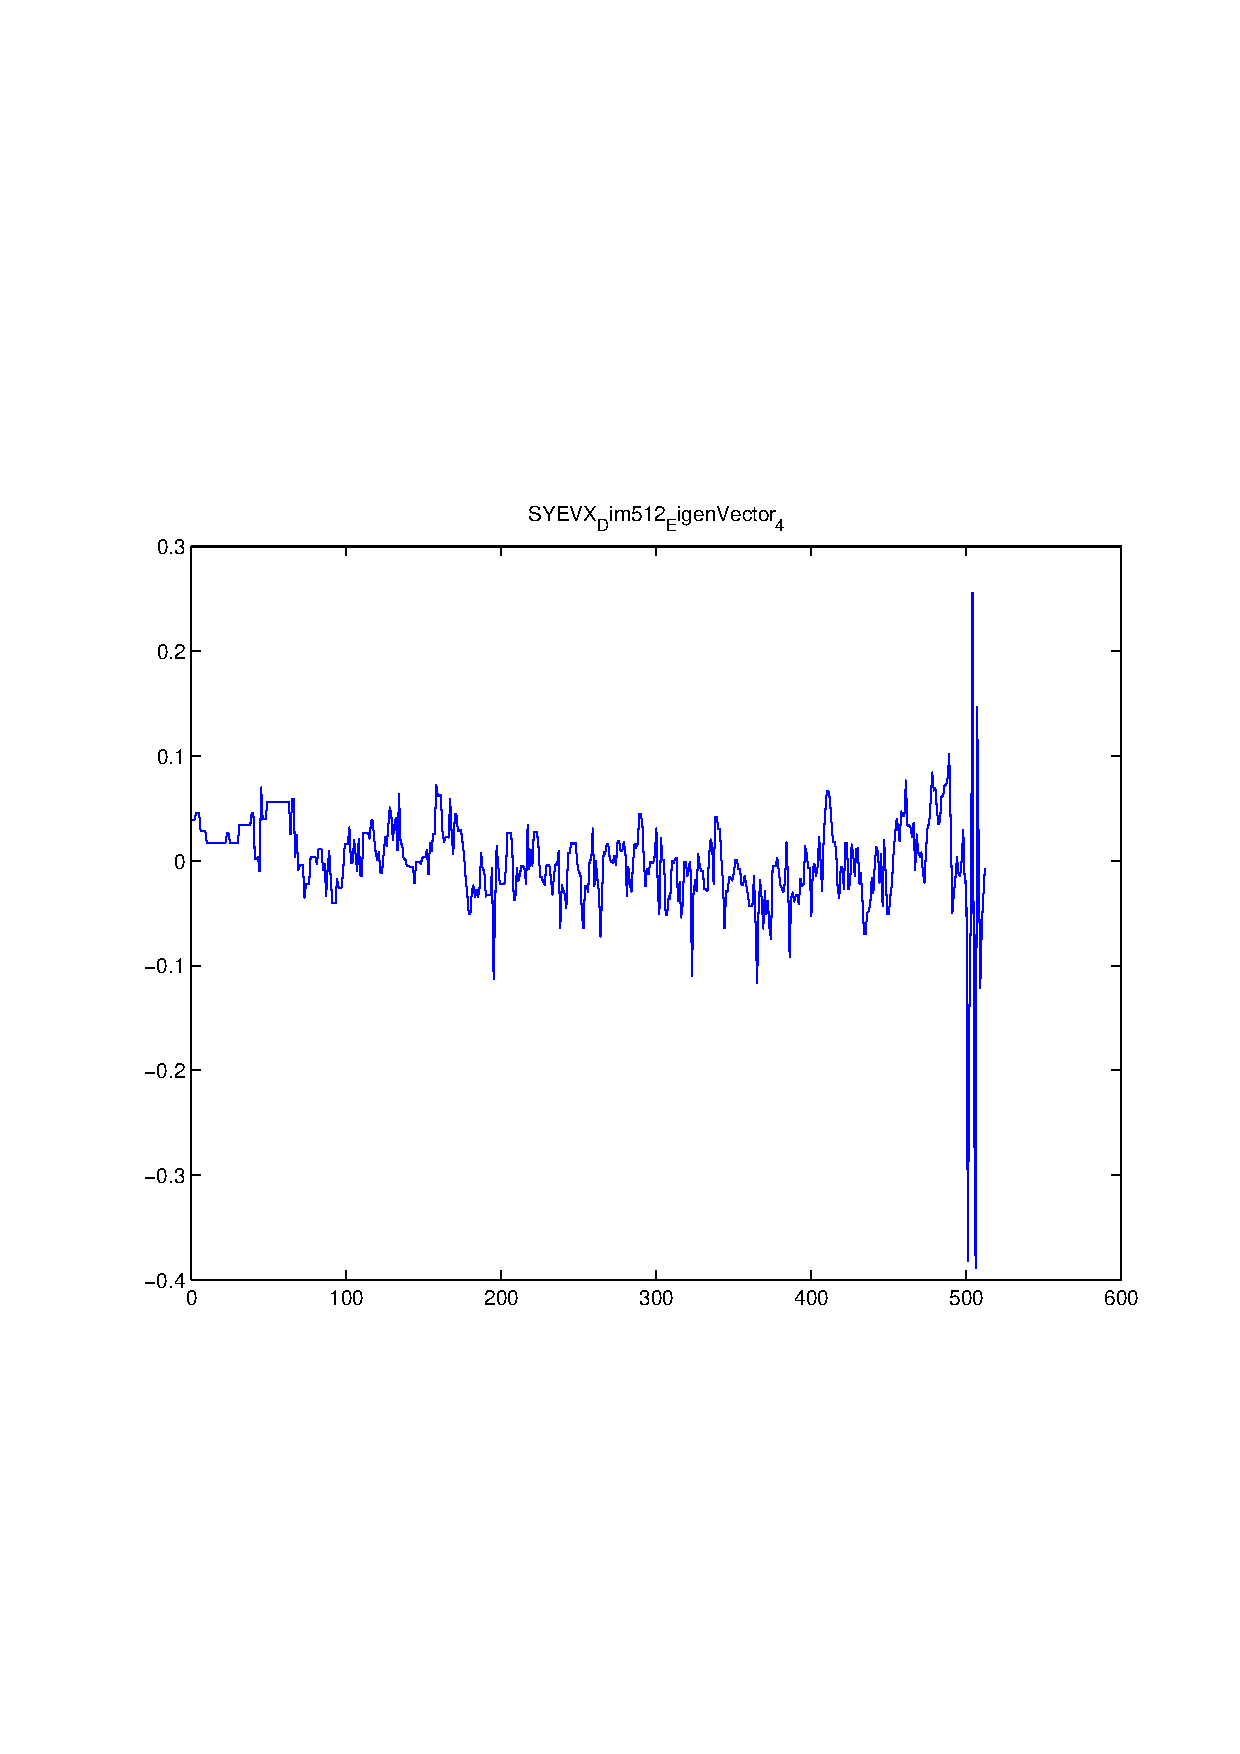
\includegraphics[width=10.0cm,height=10.0cm]{SYEVX_Dim512_EigenVector_4.pdf}

tic toc fileistream read dim n=1024 dt=66.4238
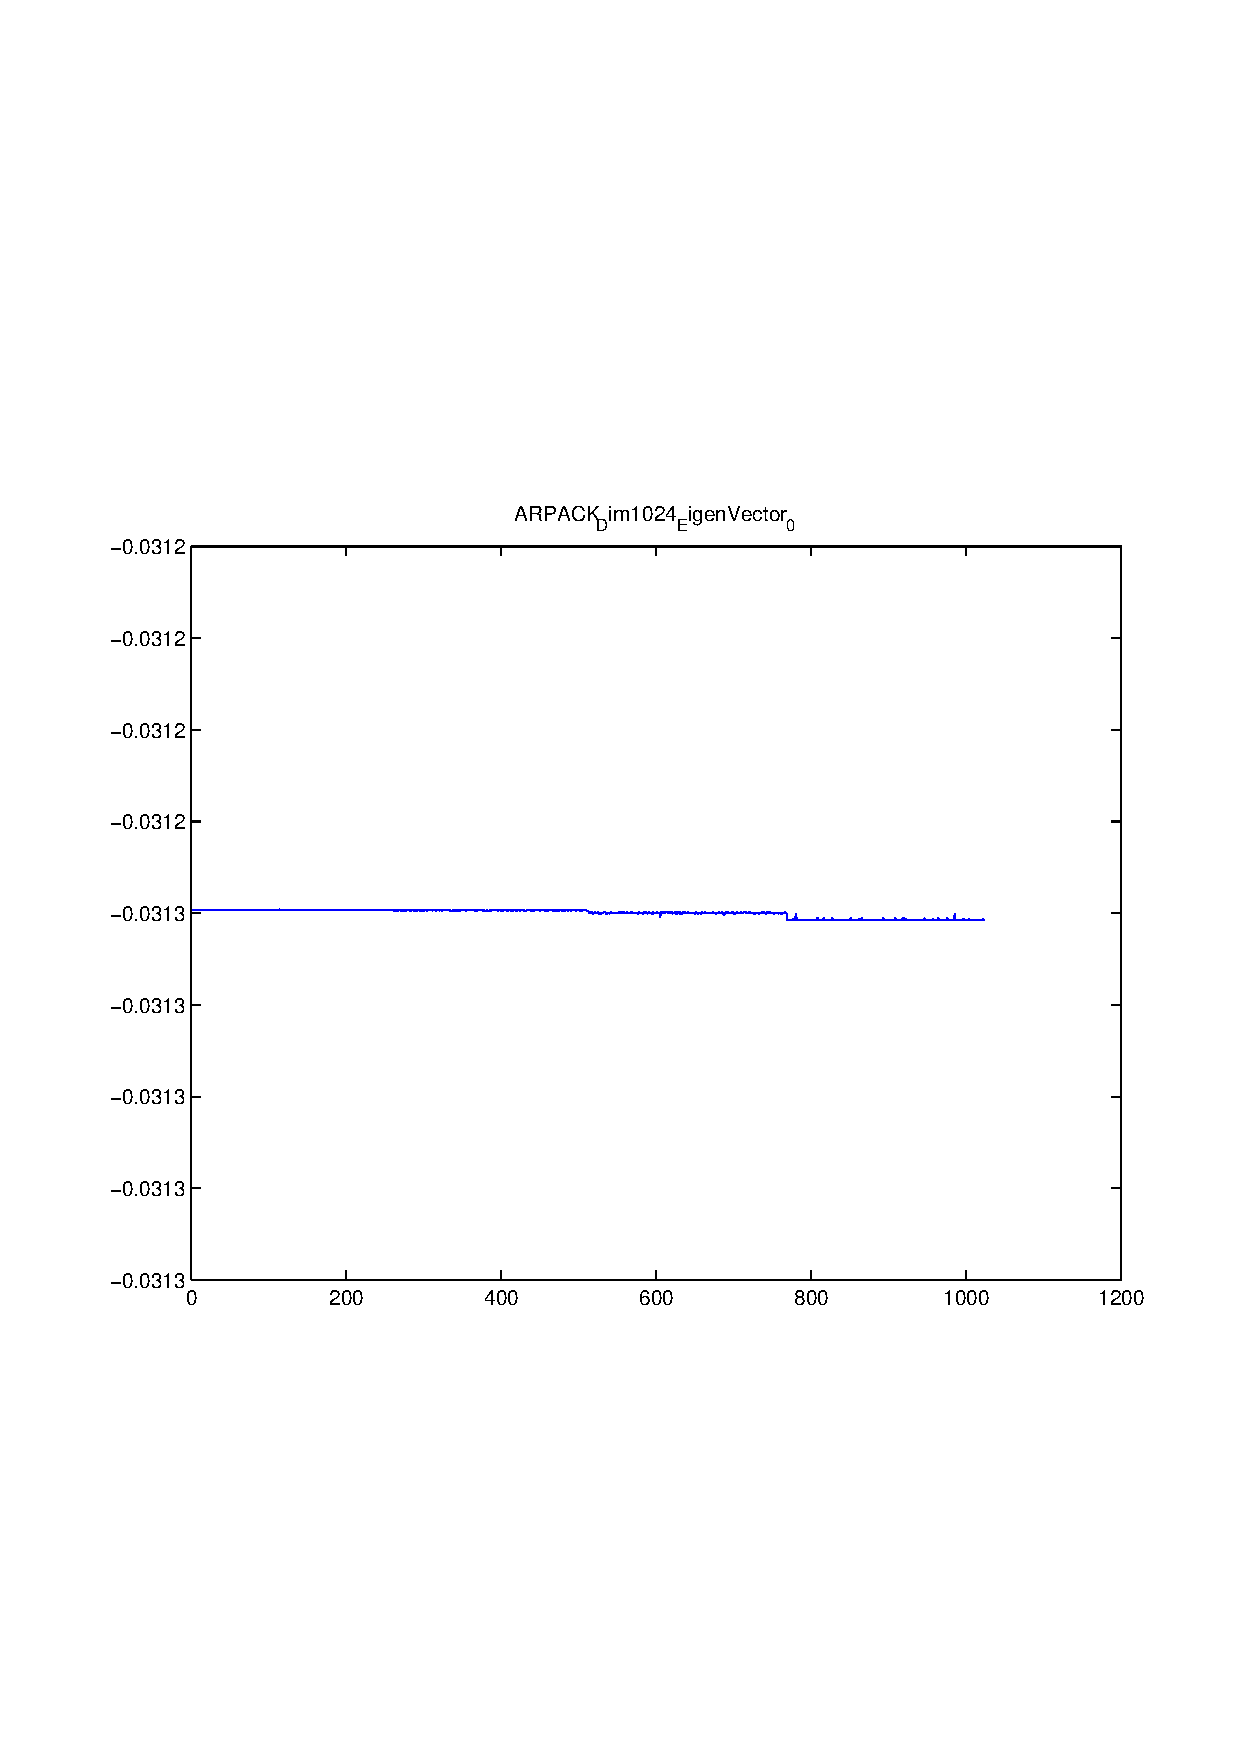
\includegraphics[width=10.0cm,height=10.0cm]{ARPACK_Dim1024_EigenVector_0.pdf}

\includegraphics[width=10.0cm,height=10.0cm]{ARPACK_Dim1024_EigenVector_1.pdf}

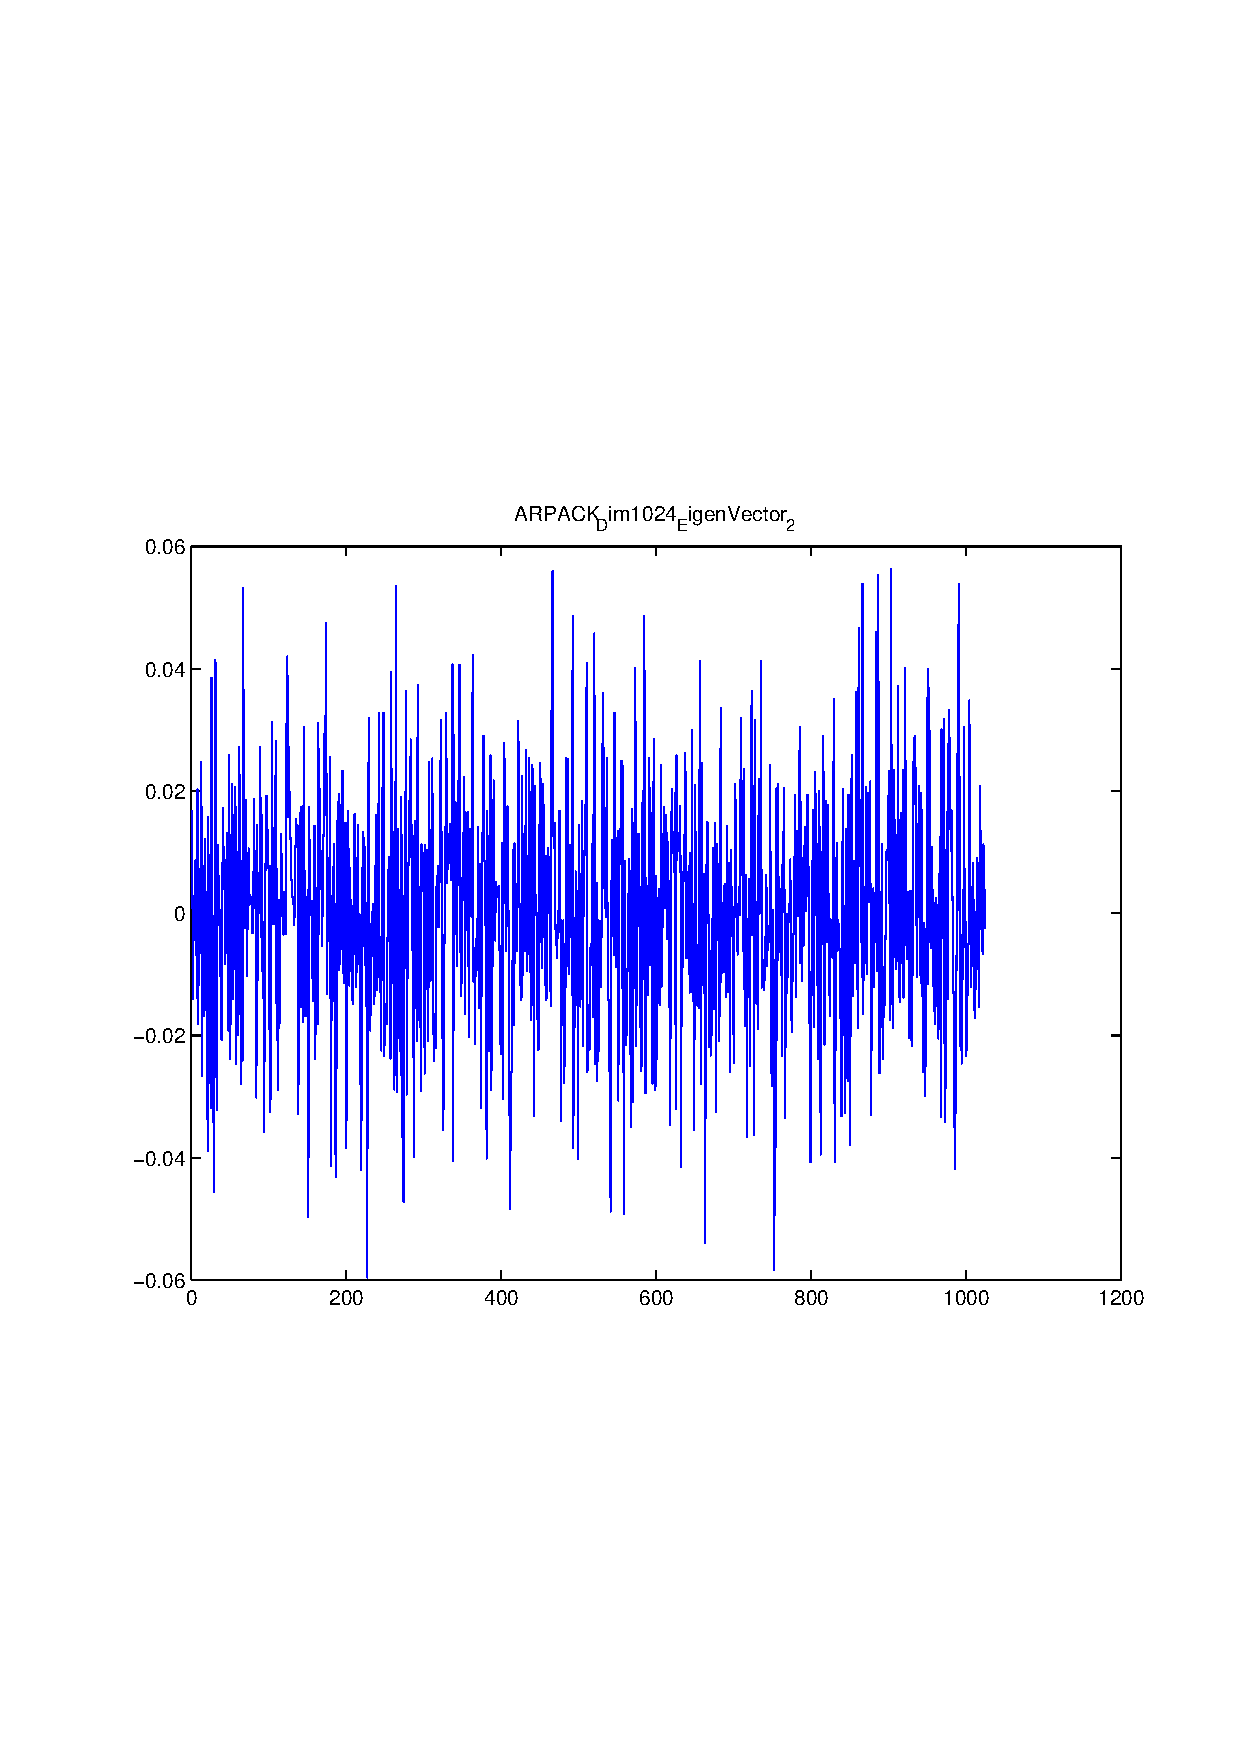
\includegraphics[width=10.0cm,height=10.0cm]{ARPACK_Dim1024_EigenVector_2.pdf}

\includegraphics[width=10.0cm,height=10.0cm]{ARPACK_Dim1024_EigenVector_3.pdf}

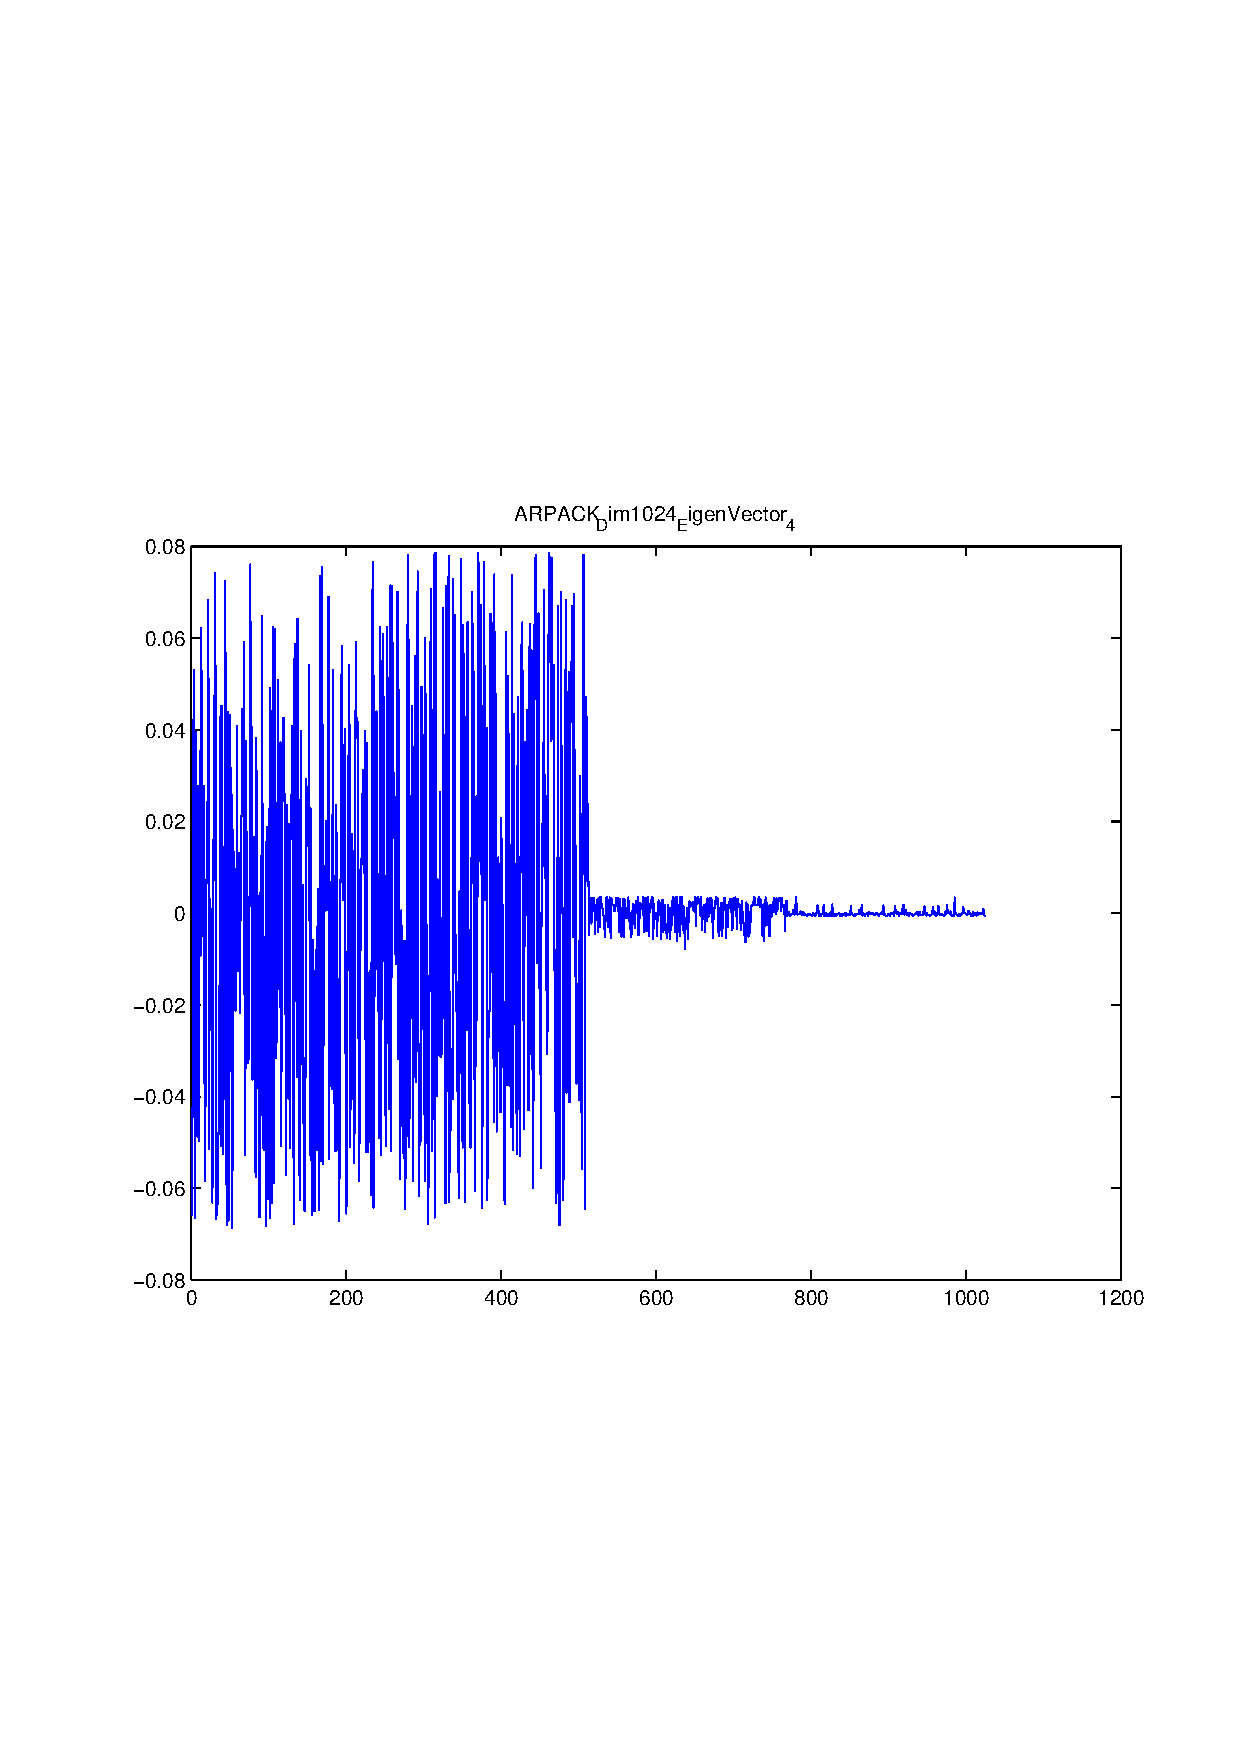
\includegraphics[width=10.0cm,height=10.0cm]{ARPACK_Dim1024_EigenVector_4.pdf}

Iterative Krylov dim=1024 dt=5.89815
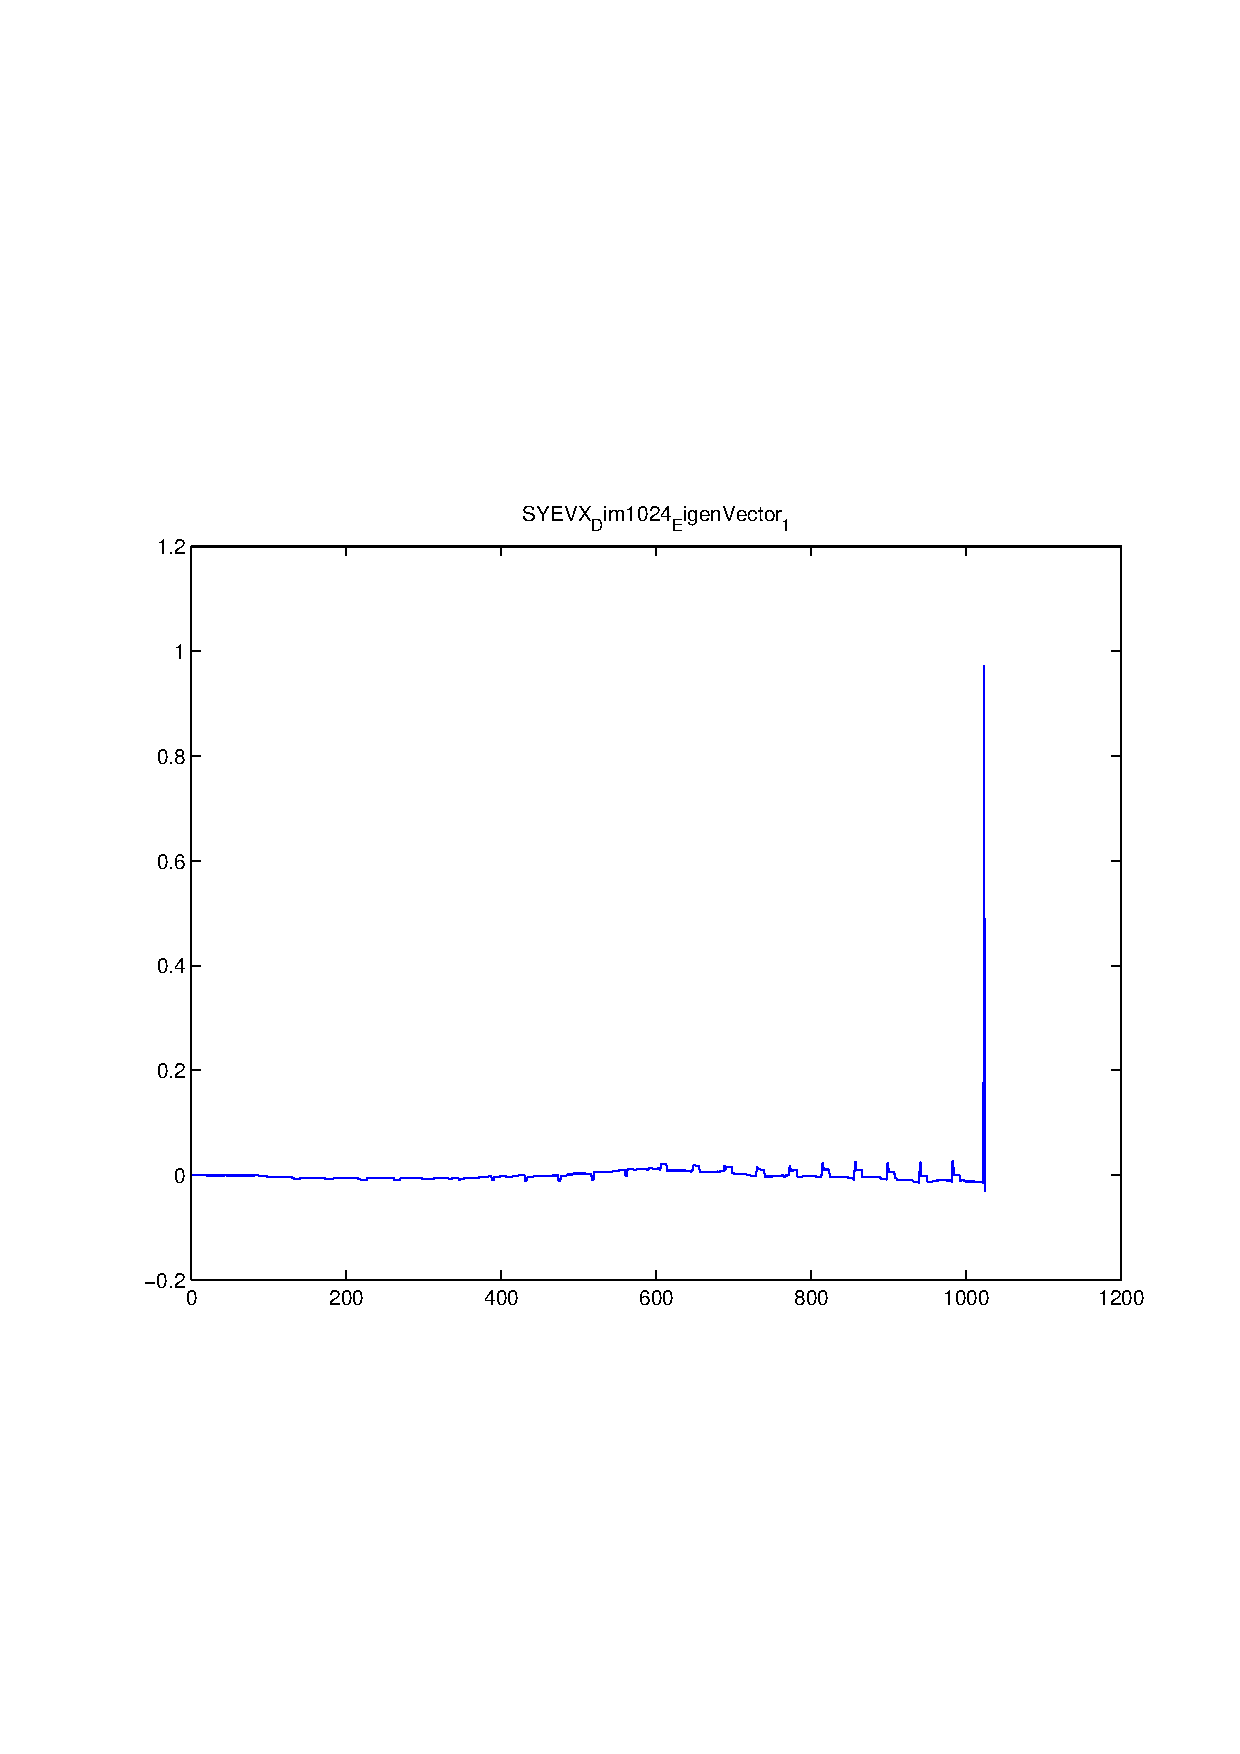
\includegraphics[width=10.0cm,height=10.0cm]{SYEVX_Dim1024_EigenVector_1.pdf}

\includegraphics[width=10.0cm,height=10.0cm]{SYEVX_Dim1024_EigenVector_2.pdf}

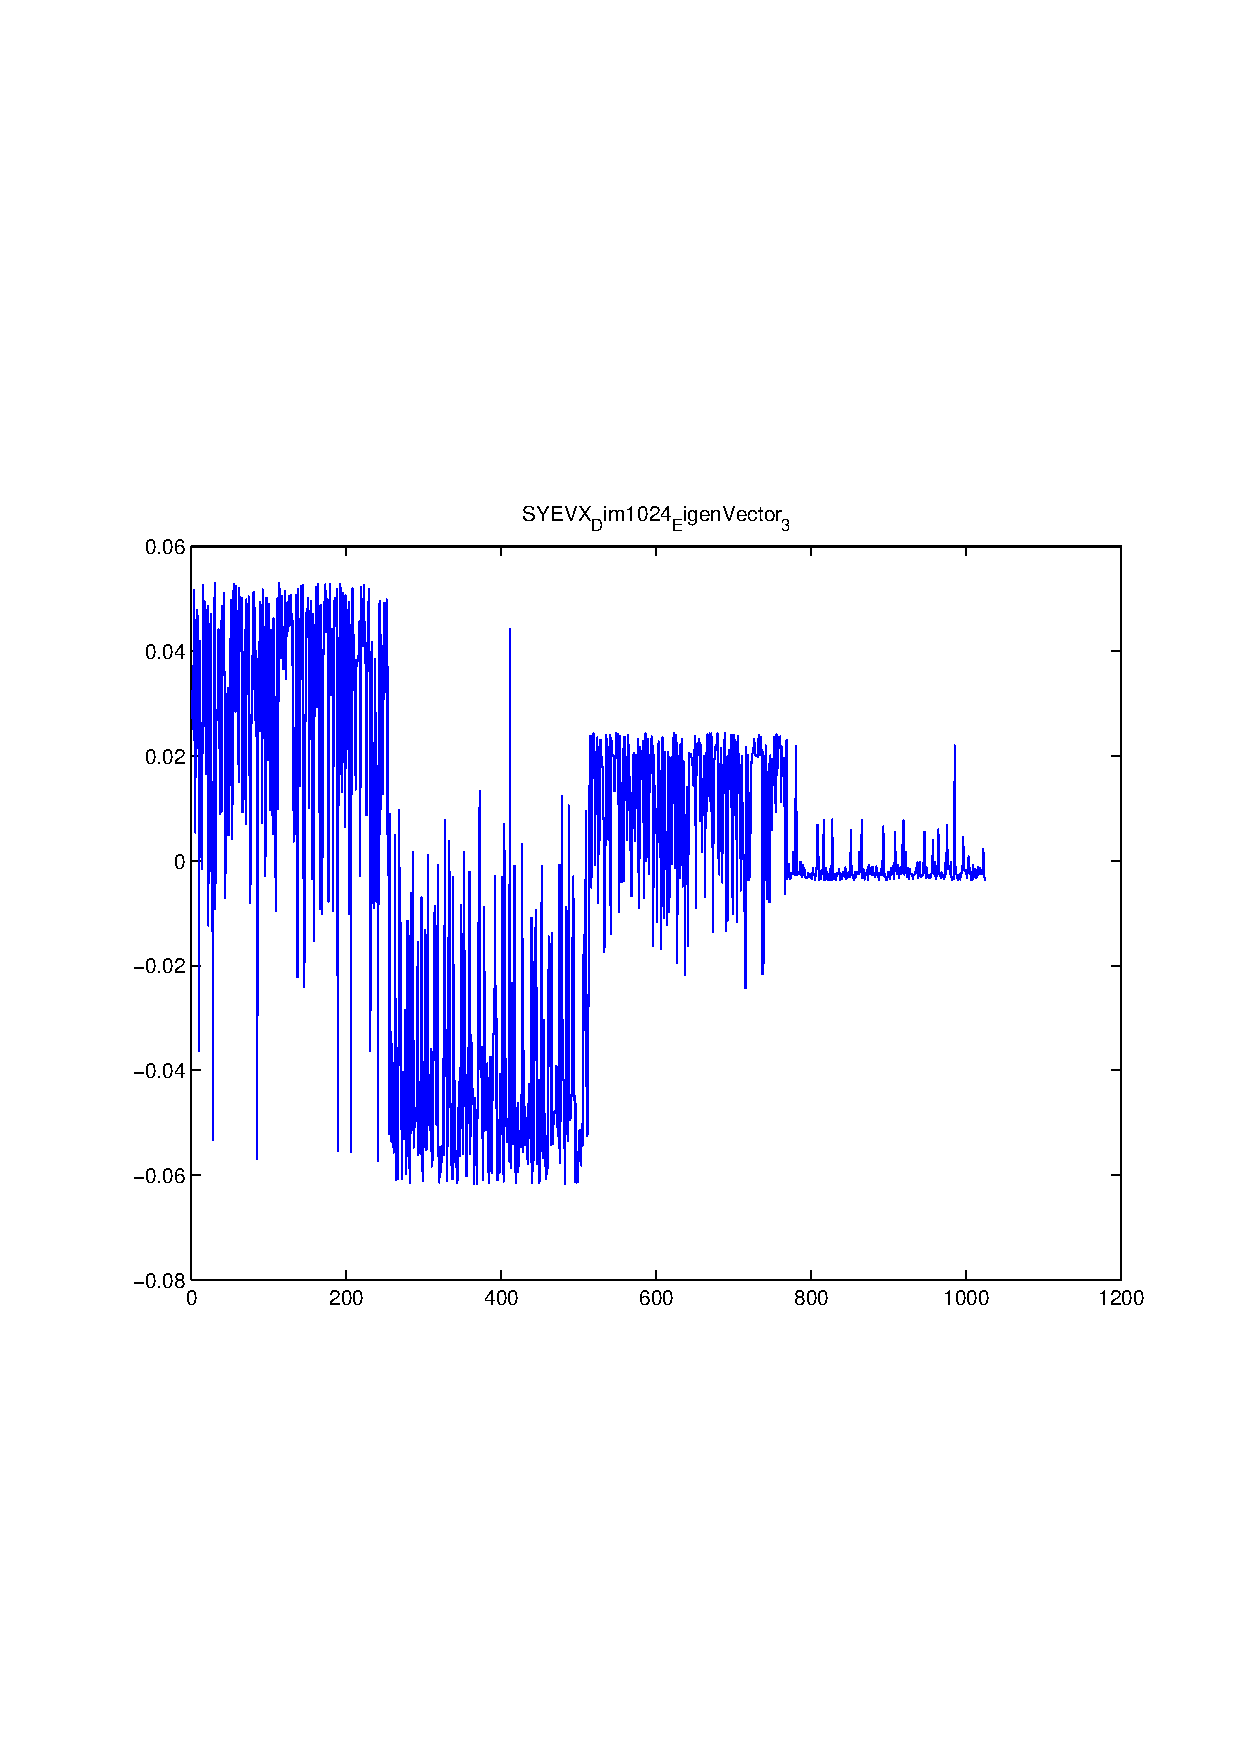
\includegraphics[width=10.0cm,height=10.0cm]{SYEVX_Dim1024_EigenVector_3.pdf}

\includegraphics[width=10.0cm,height=10.0cm]{SYEVX_Dim1024_EigenVector_4.pdf}

tic toc fileistream read dim n=2048 dt=57.5512
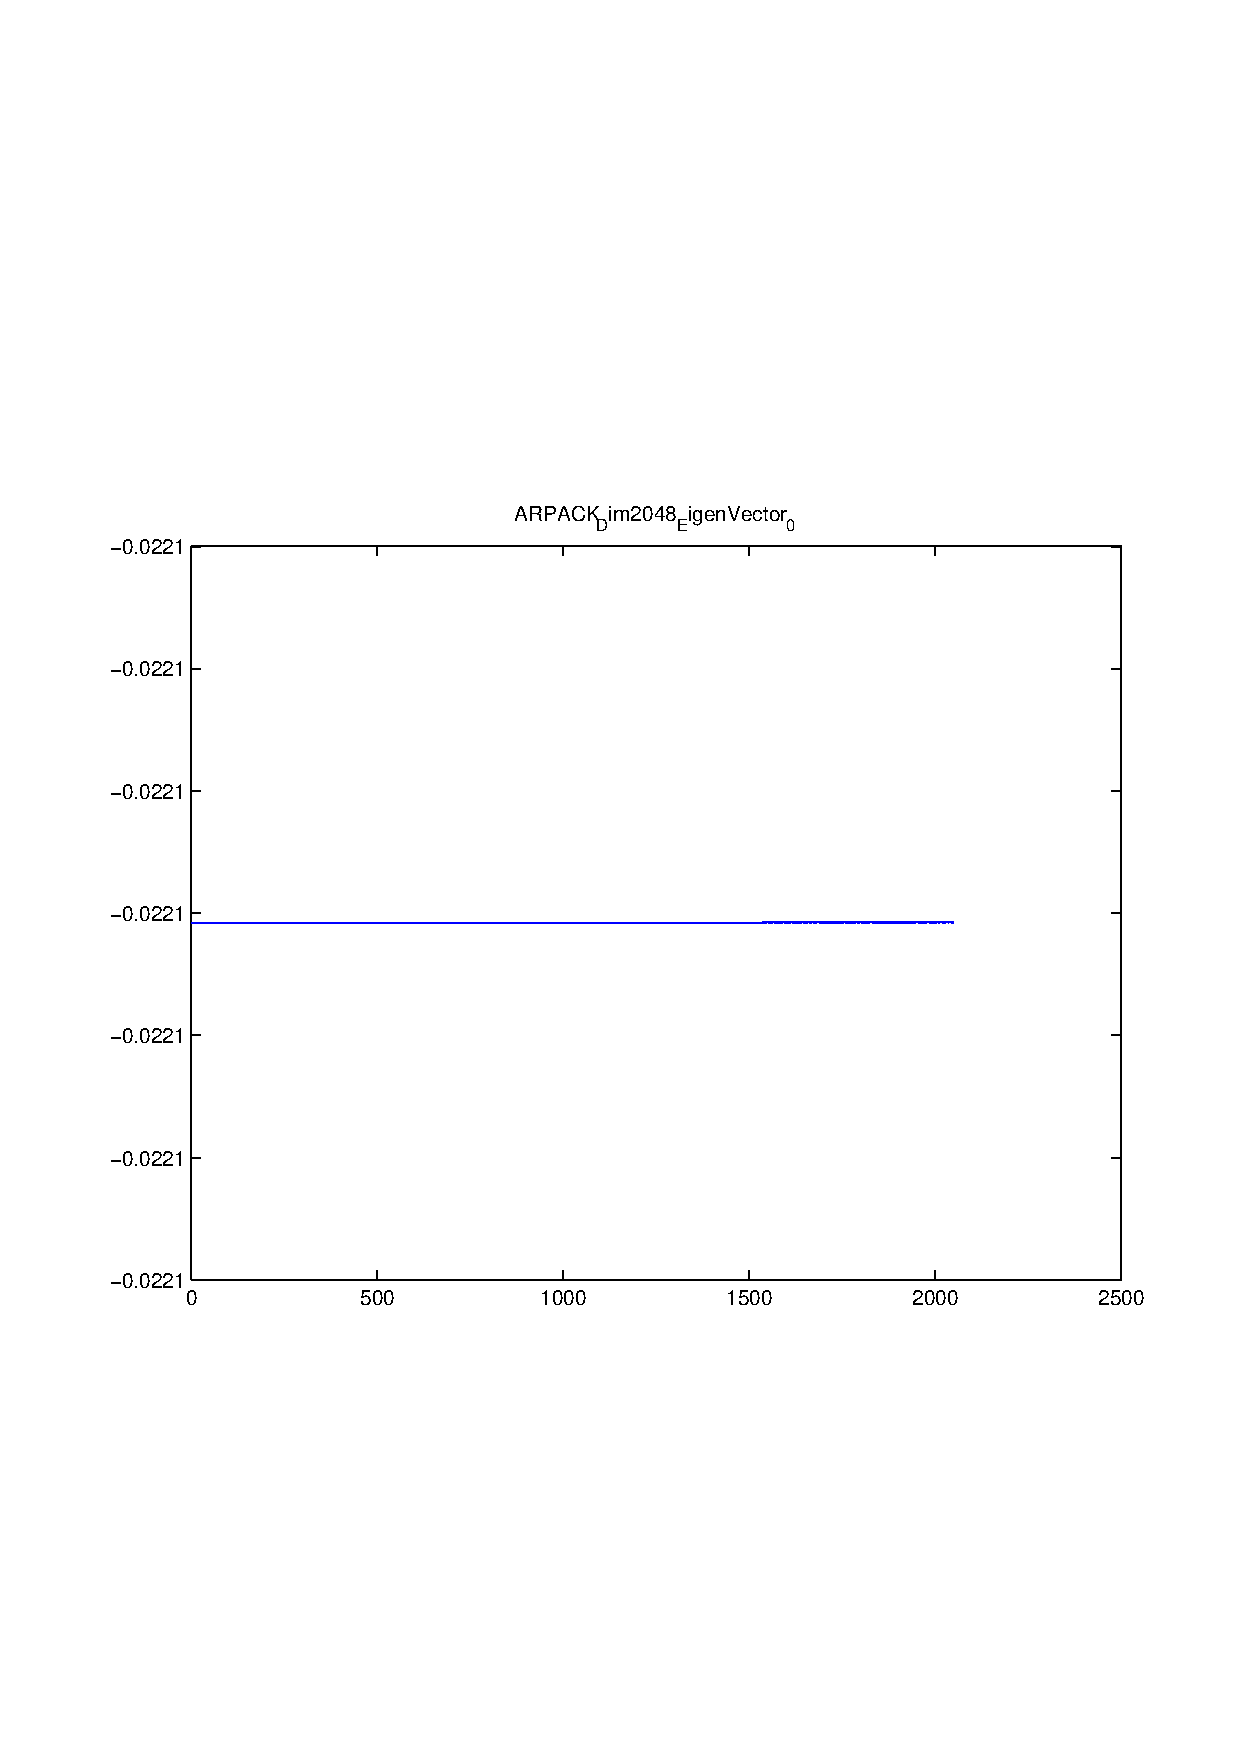
\includegraphics[width=10.0cm,height=10.0cm]{ARPACK_Dim2048_EigenVector_0.pdf}

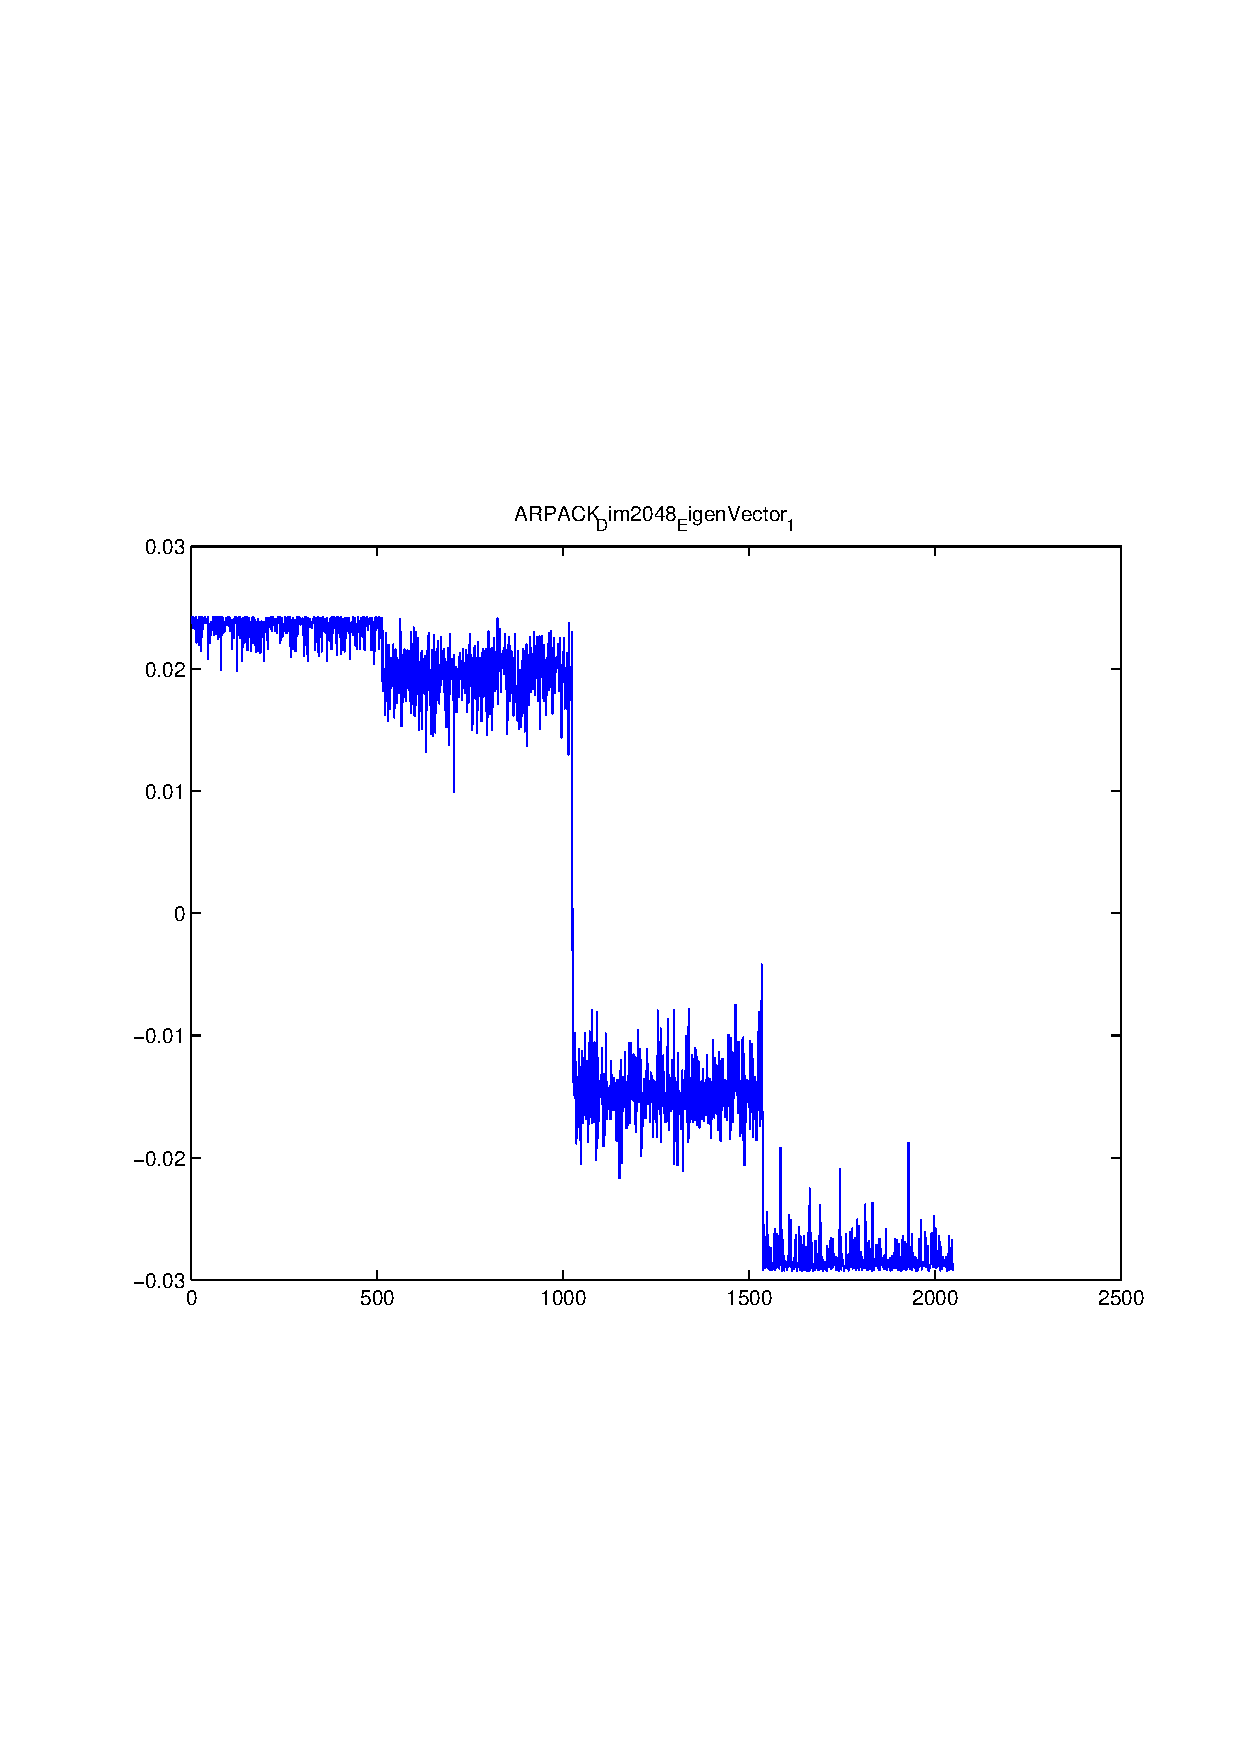
\includegraphics[width=10.0cm,height=10.0cm]{ARPACK_Dim2048_EigenVector_1.pdf}

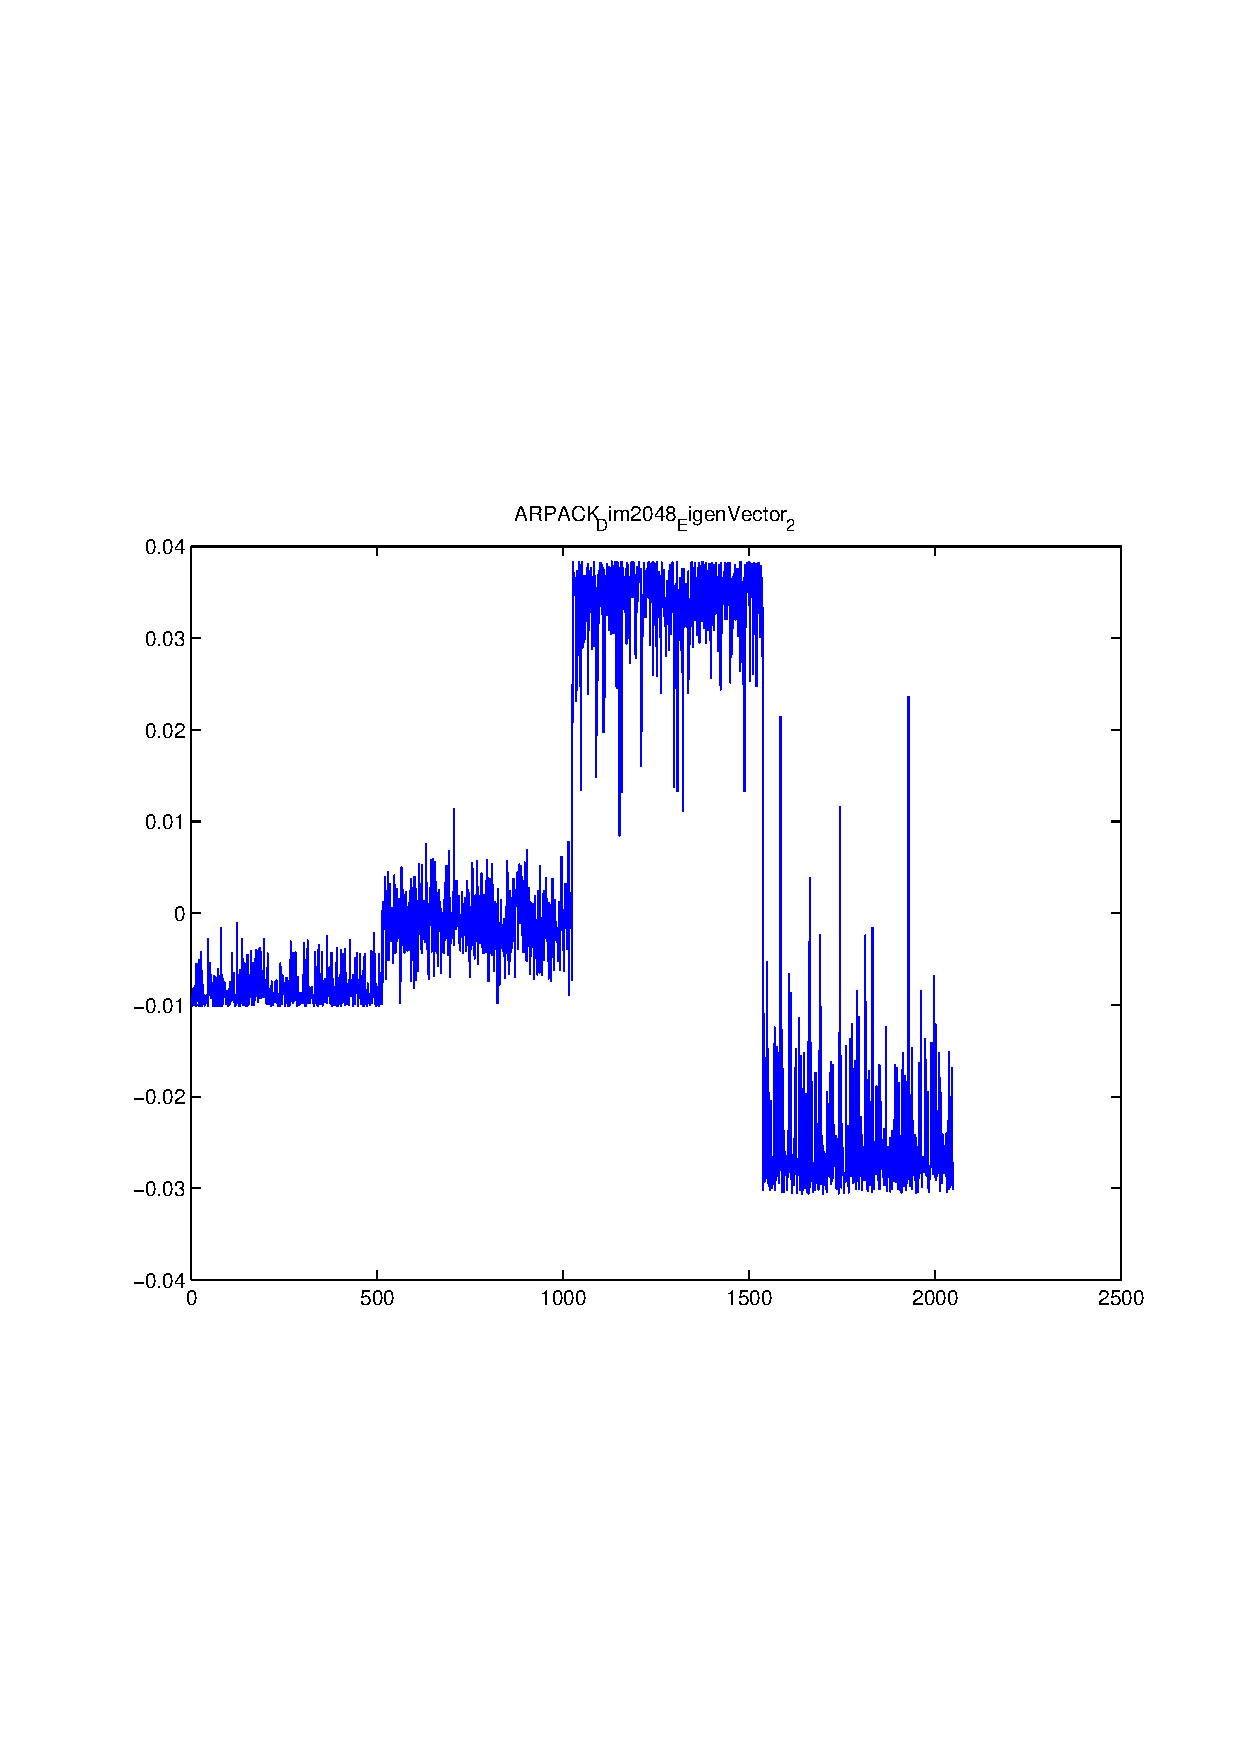
\includegraphics[width=10.0cm,height=10.0cm]{ARPACK_Dim2048_EigenVector_2.pdf}

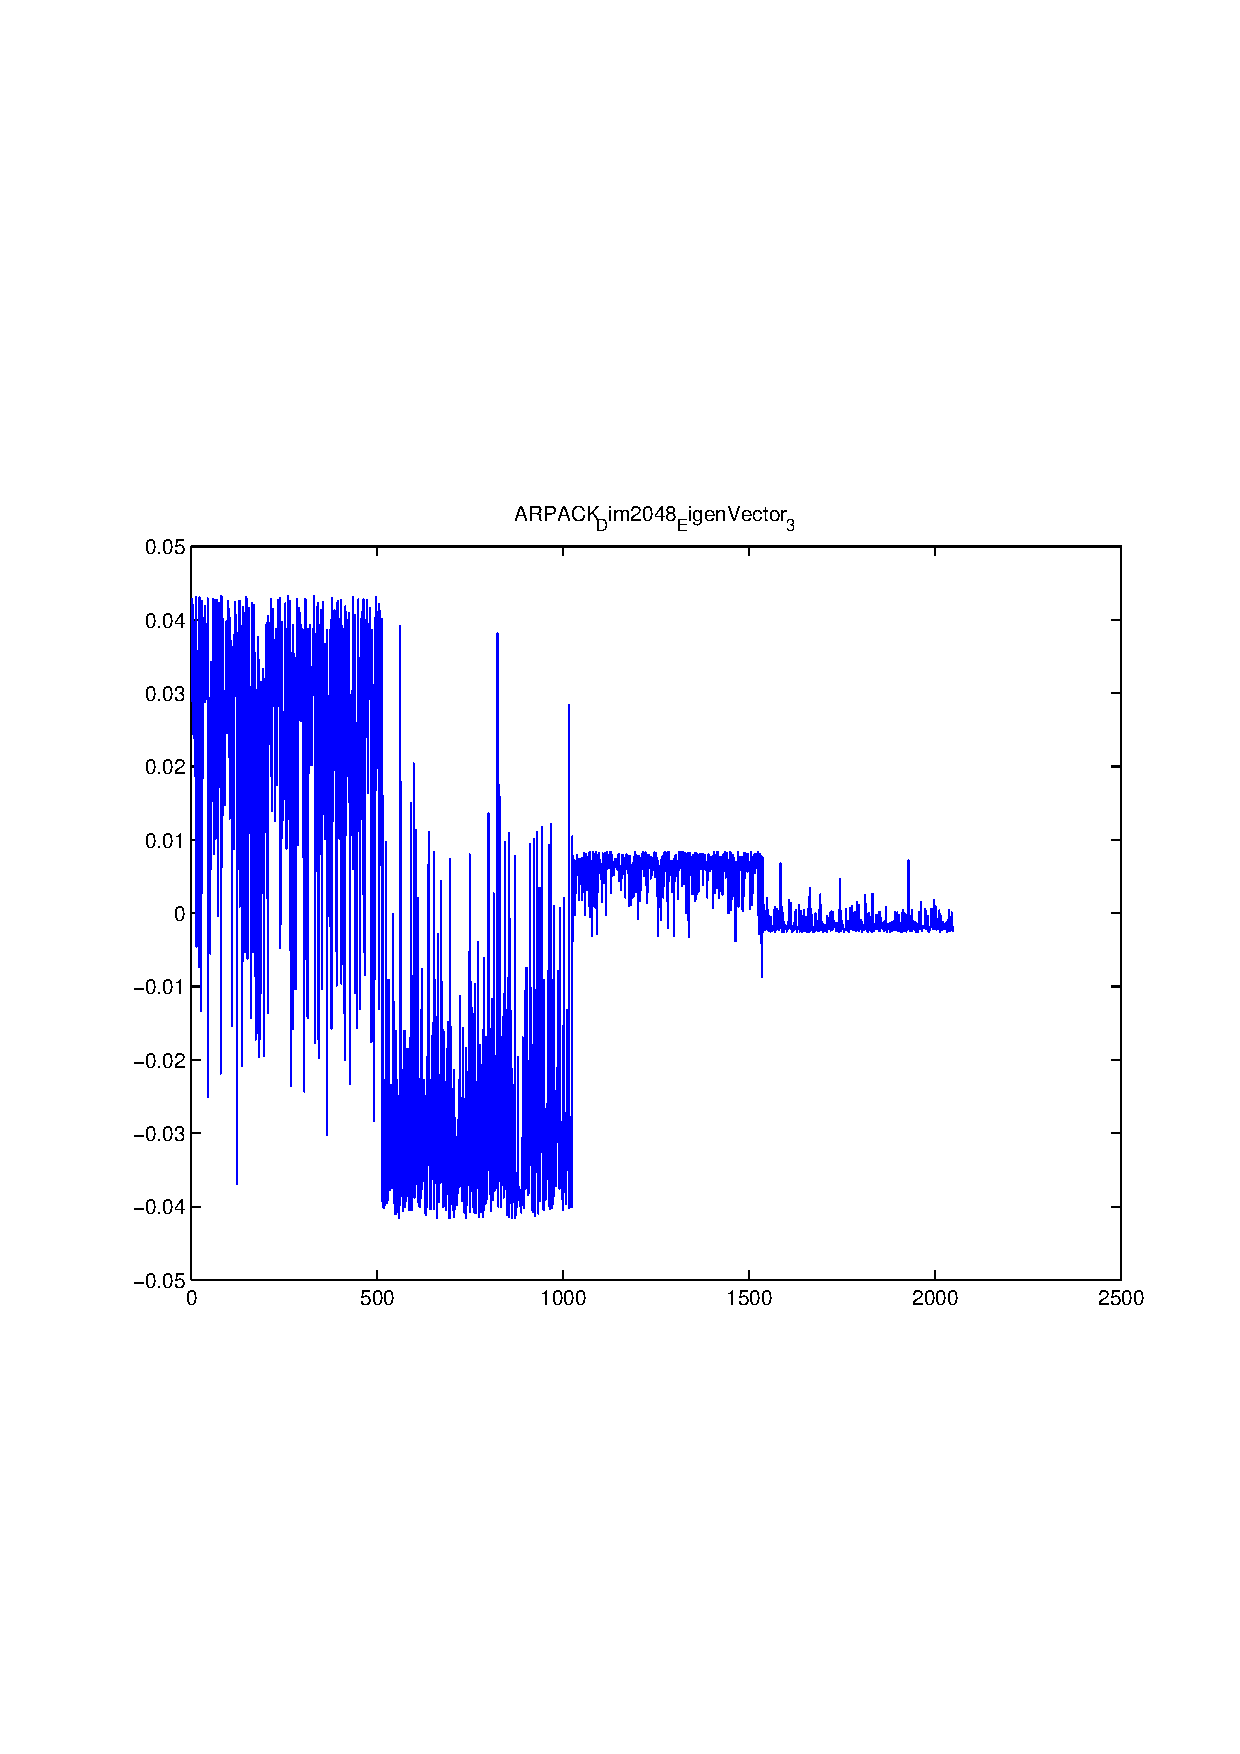
\includegraphics[width=10.0cm,height=10.0cm]{ARPACK_Dim2048_EigenVector_3.pdf}

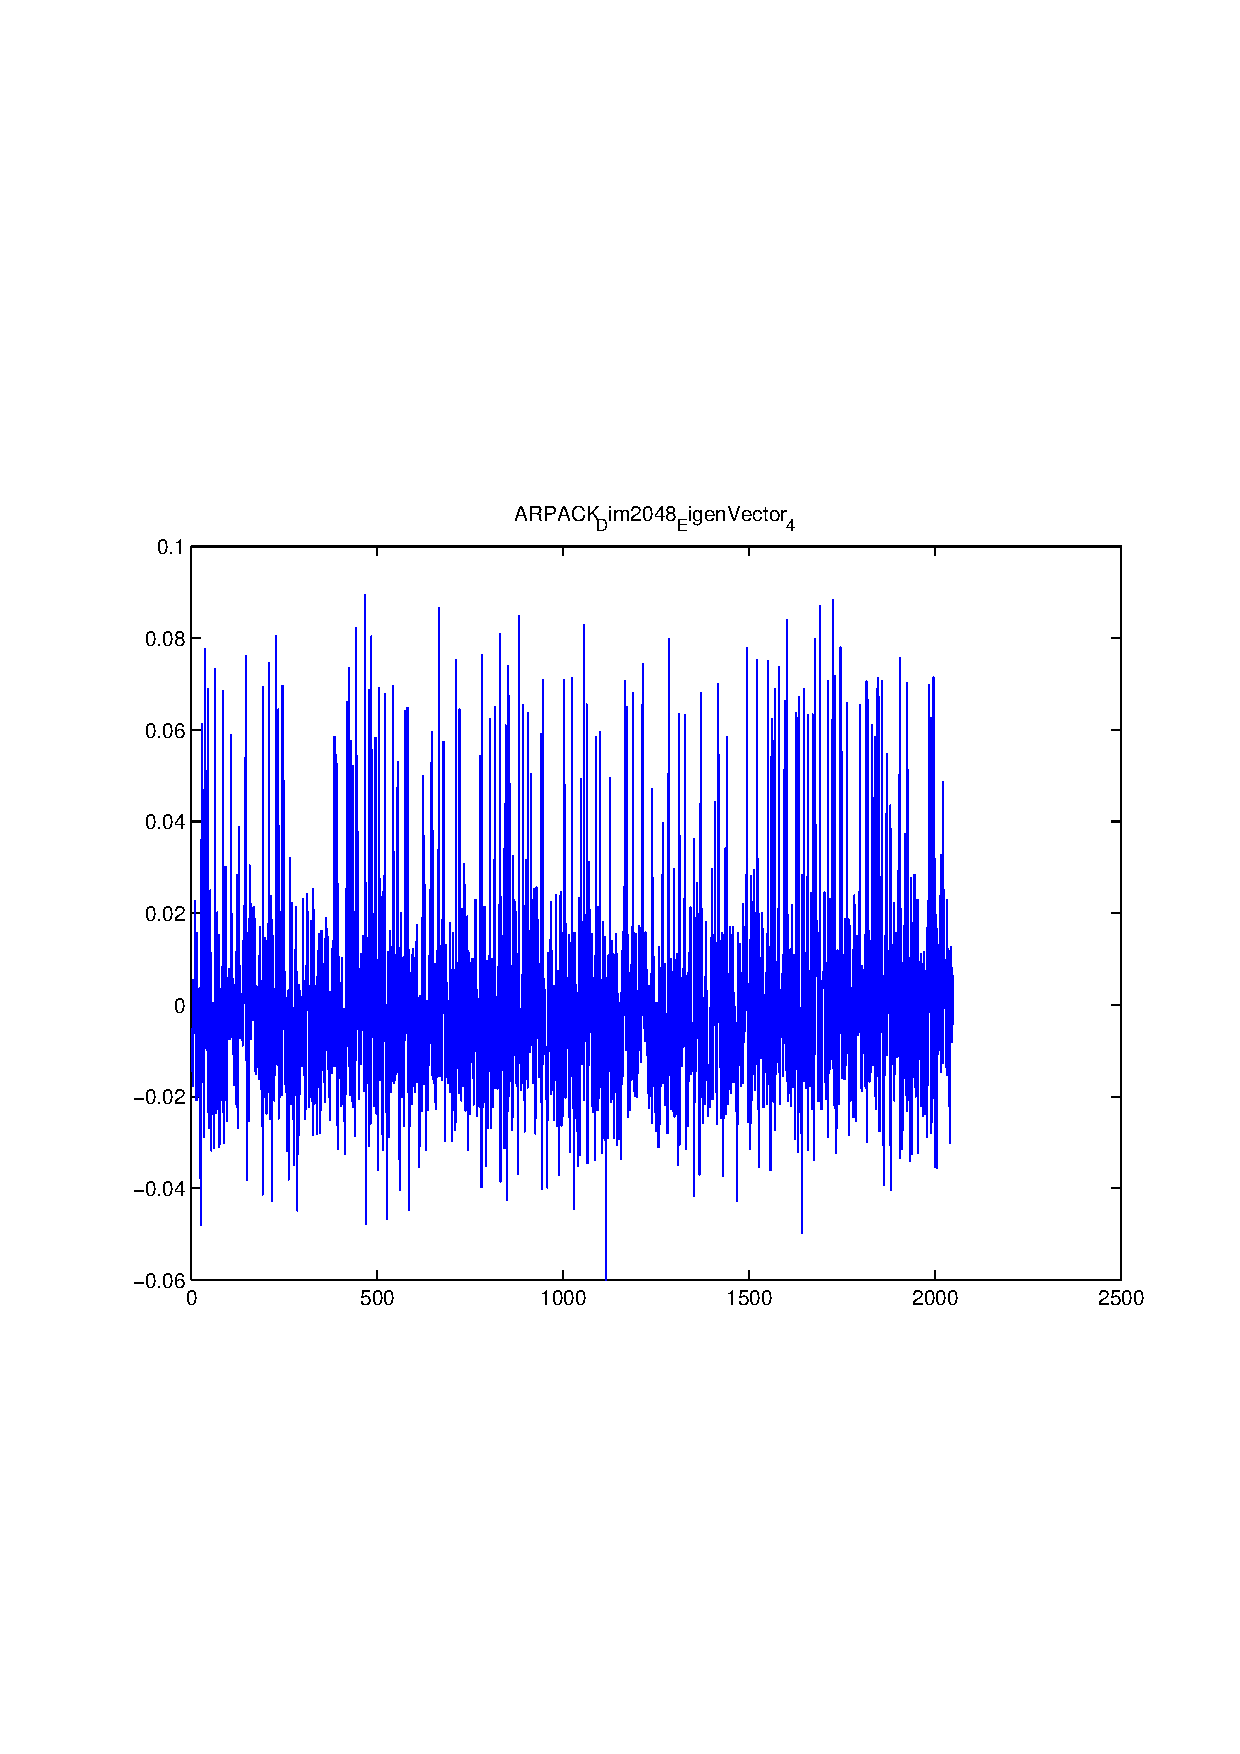
\includegraphics[width=10.0cm,height=10.0cm]{ARPACK_Dim2048_EigenVector_4.pdf}

Iterative Krylov dim=2048 dt=6.66393
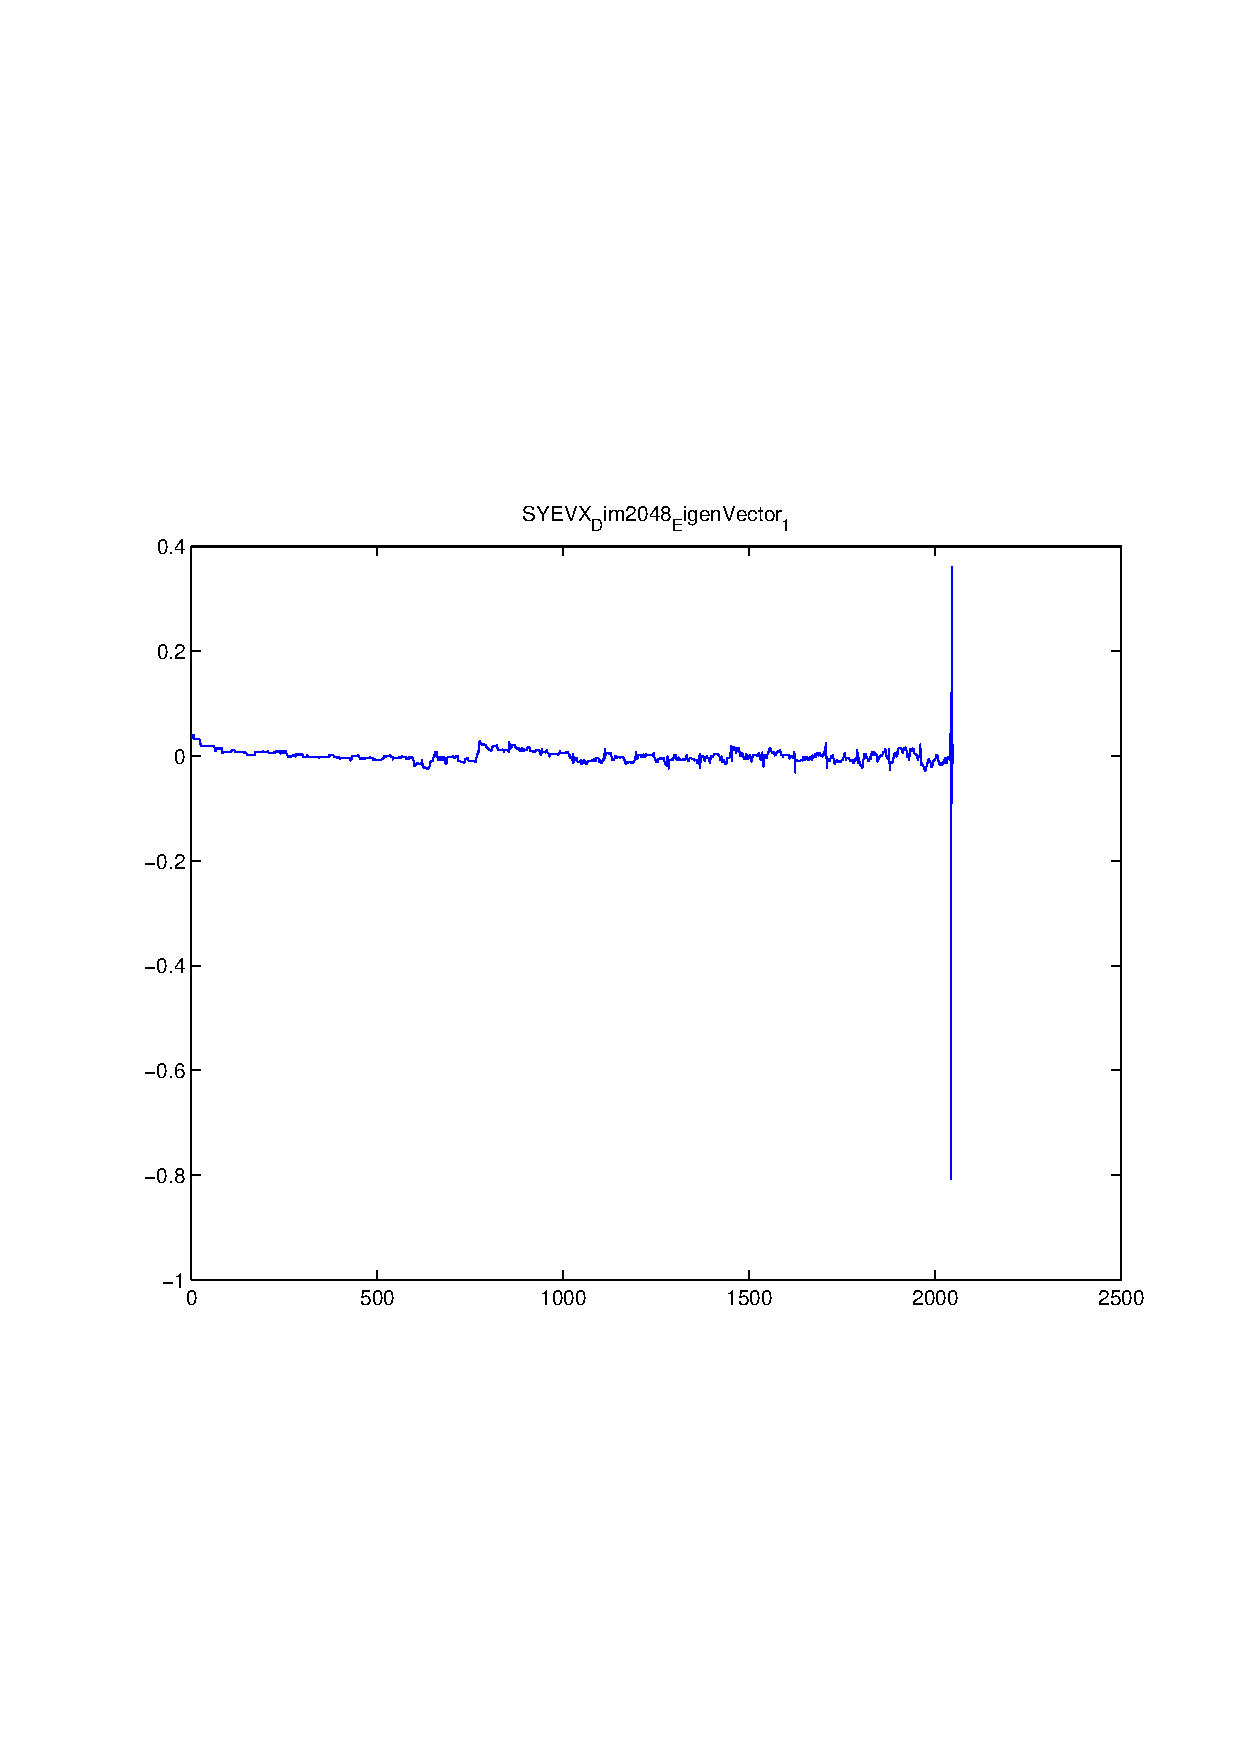
\includegraphics[width=10.0cm,height=10.0cm]{SYEVX_Dim2048_EigenVector_1.pdf}

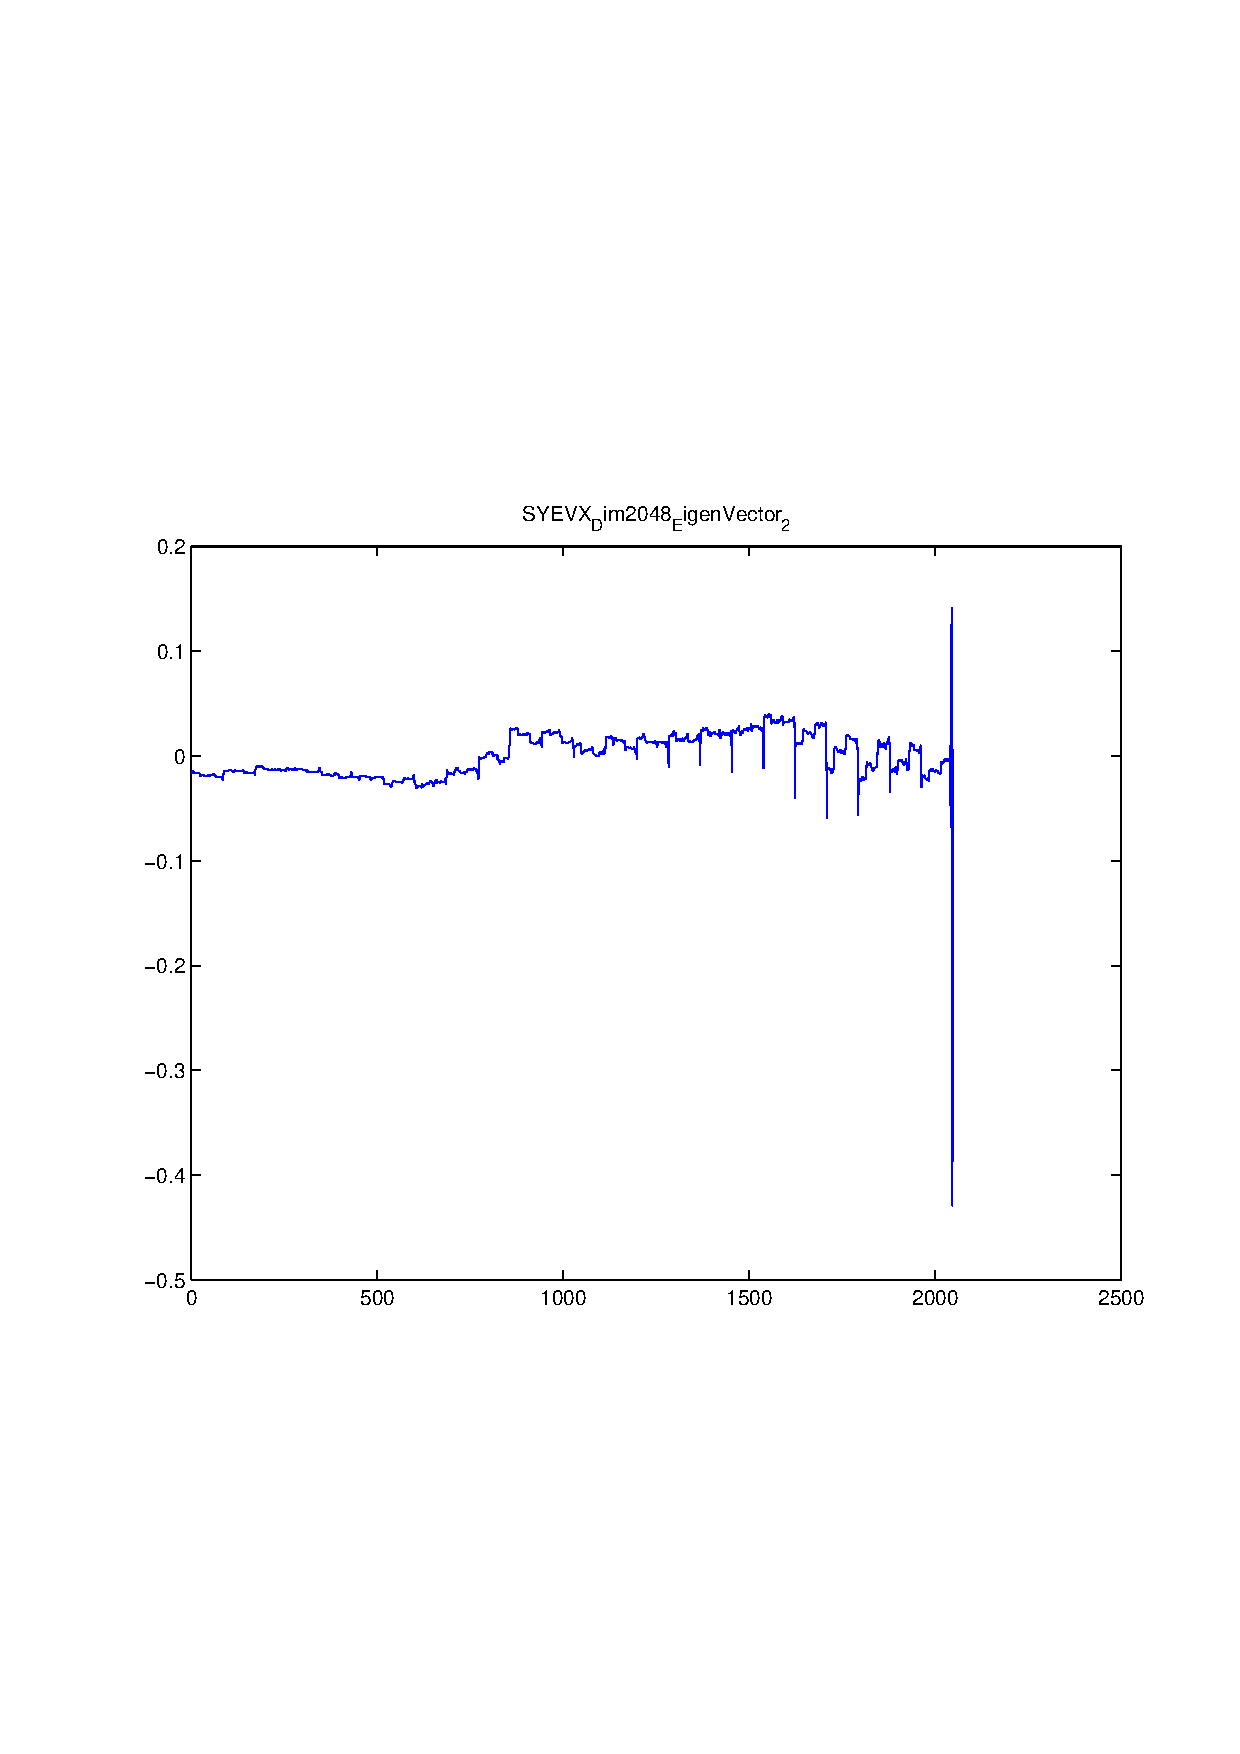
\includegraphics[width=10.0cm,height=10.0cm]{SYEVX_Dim2048_EigenVector_2.pdf}

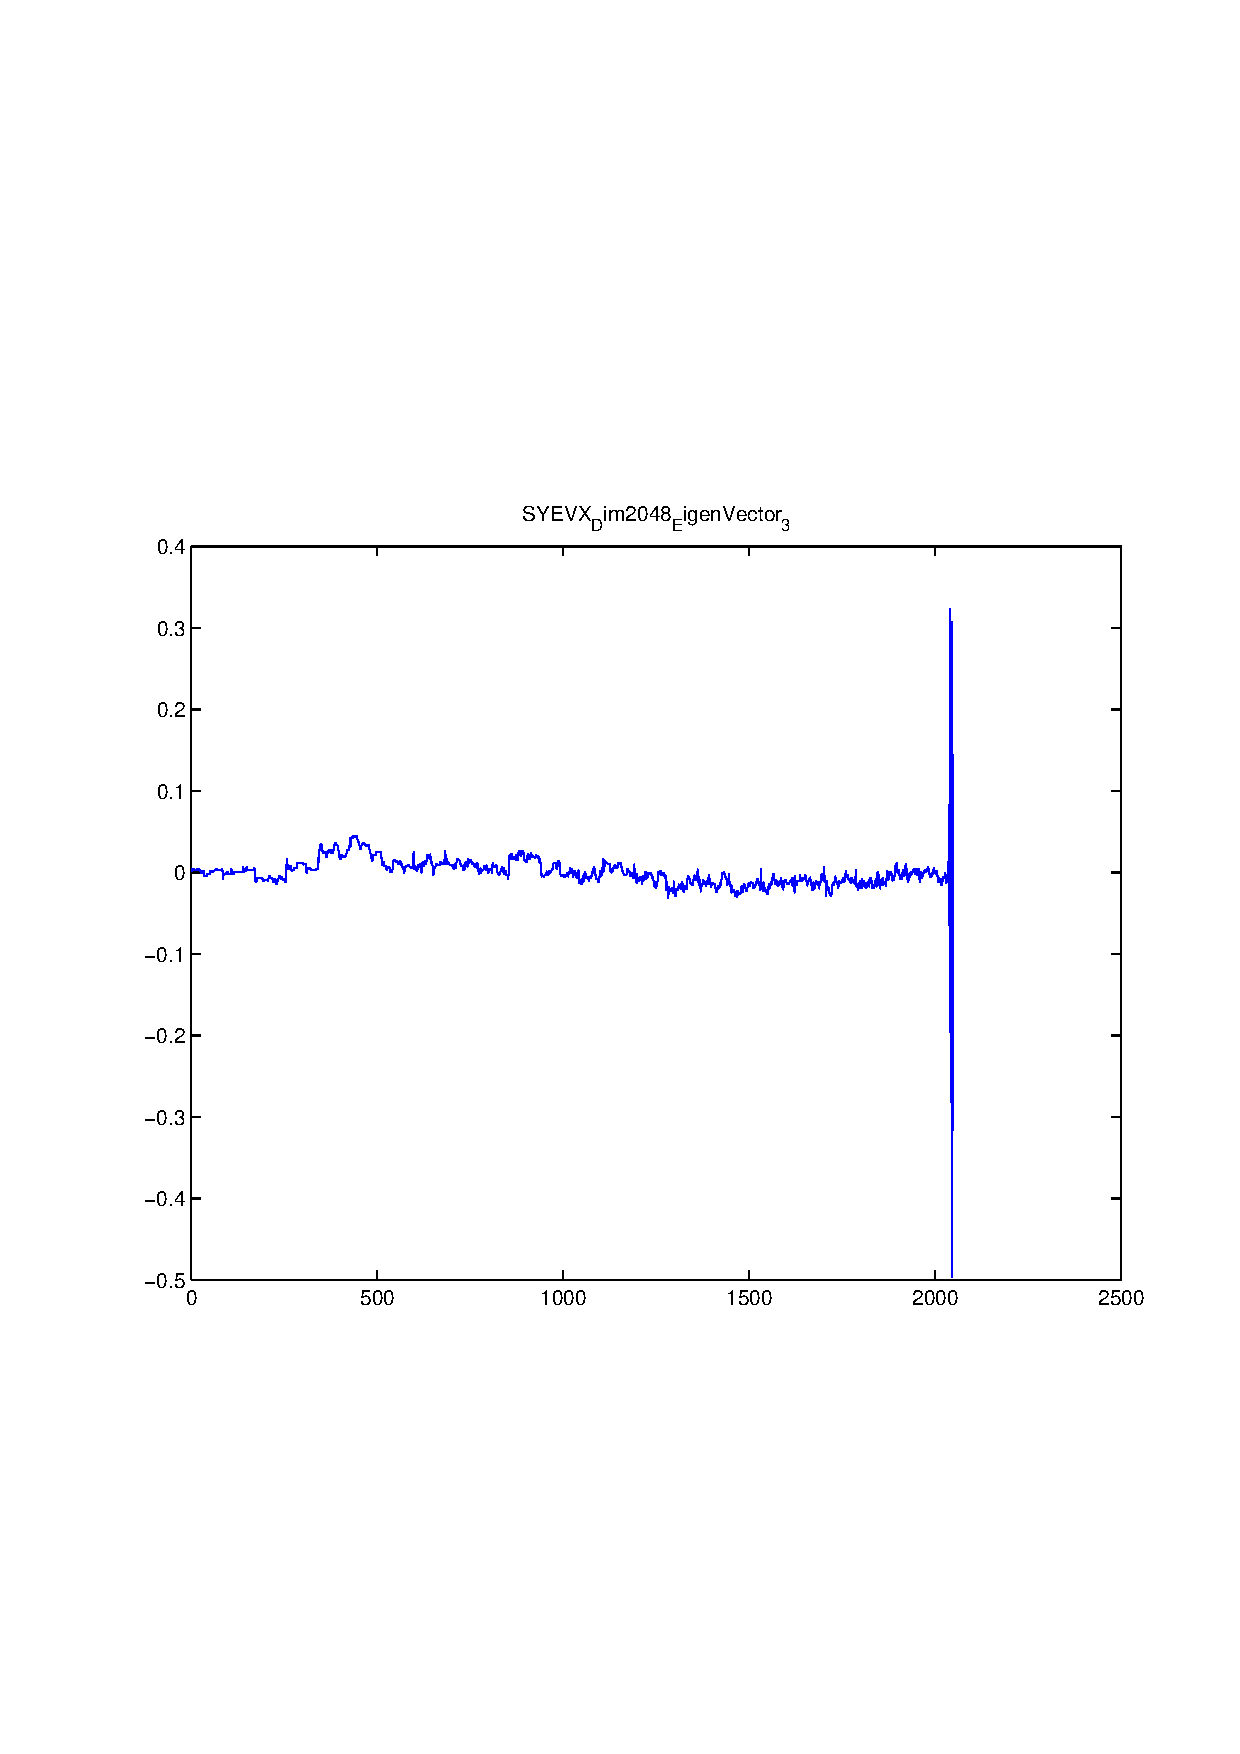
\includegraphics[width=10.0cm,height=10.0cm]{SYEVX_Dim2048_EigenVector_3.pdf}

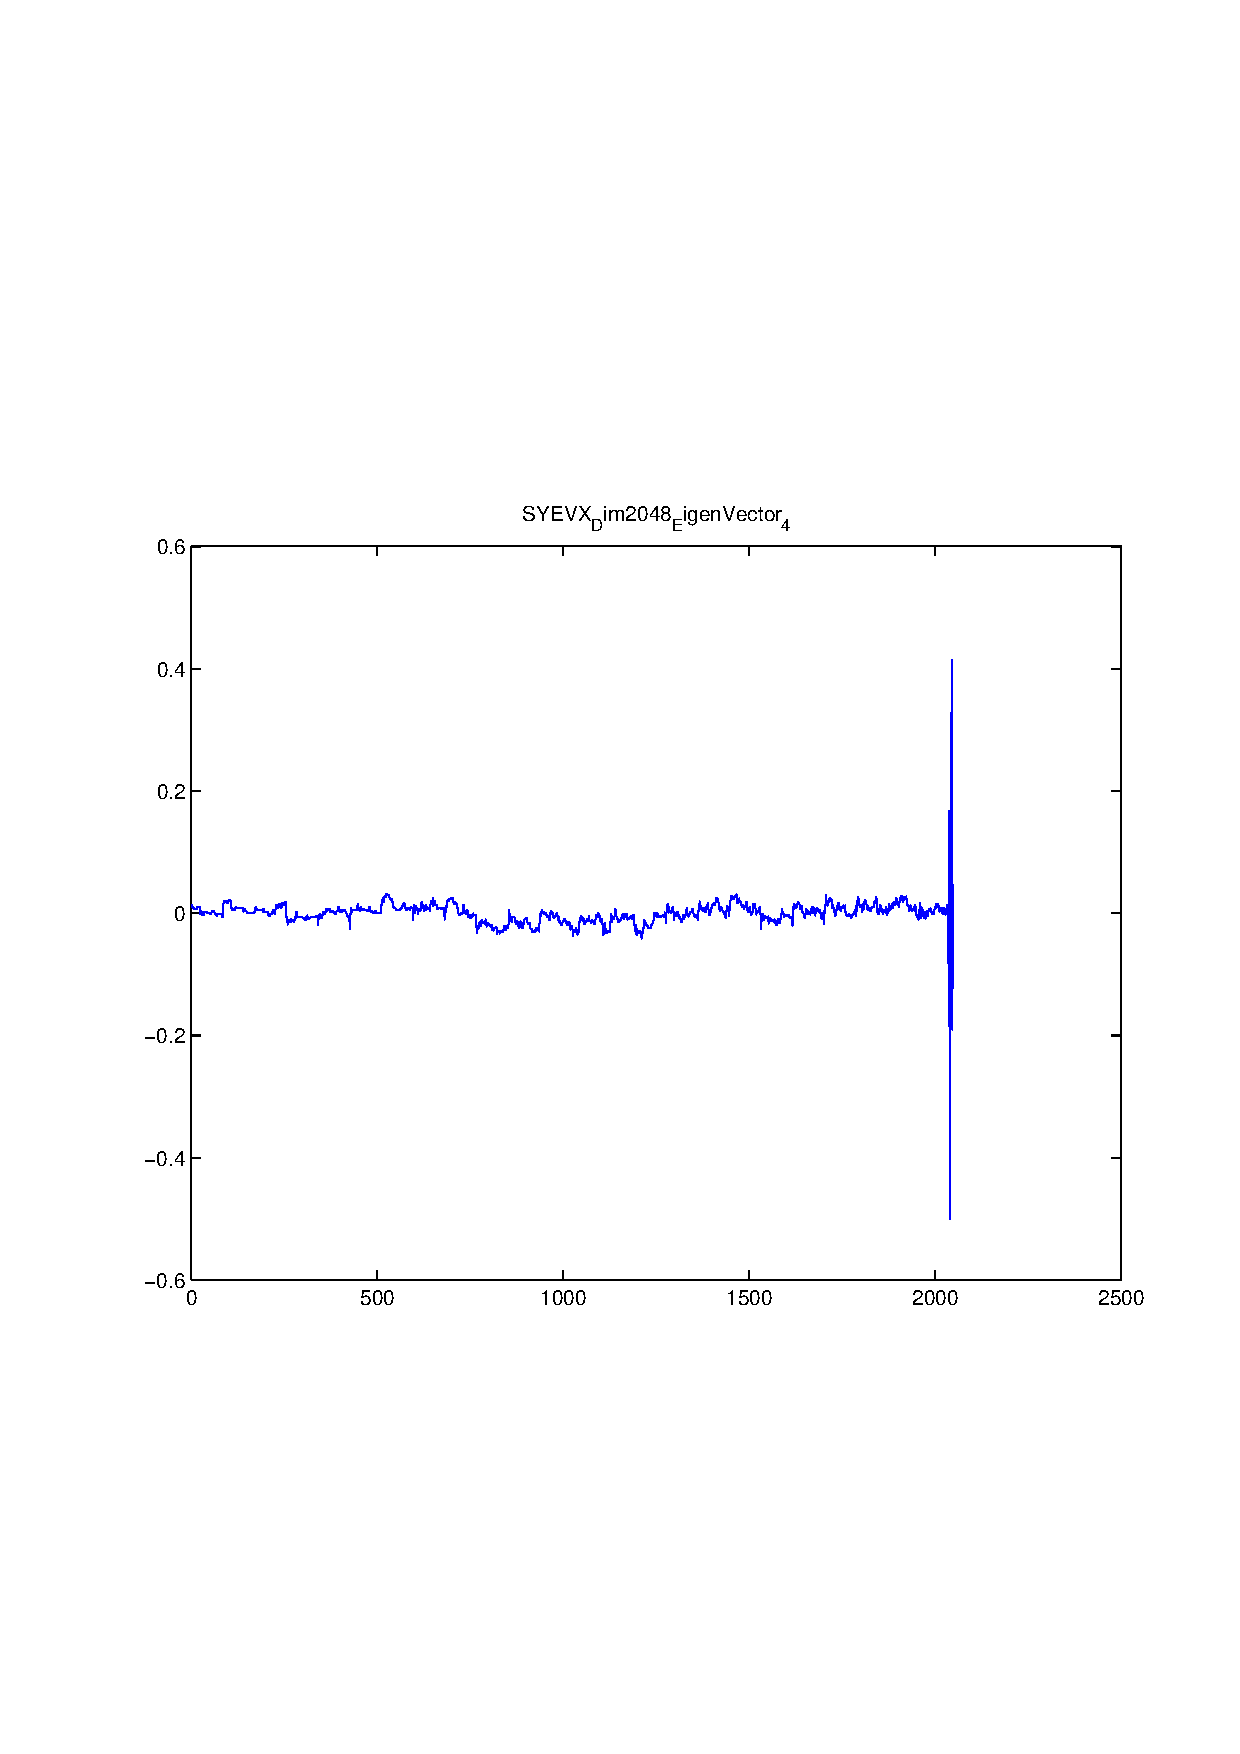
\includegraphics[width=10.0cm,height=10.0cm]{SYEVX_Dim2048_EigenVector_4.pdf}

tic toc fileistream read dim n=4096 dt=125.039
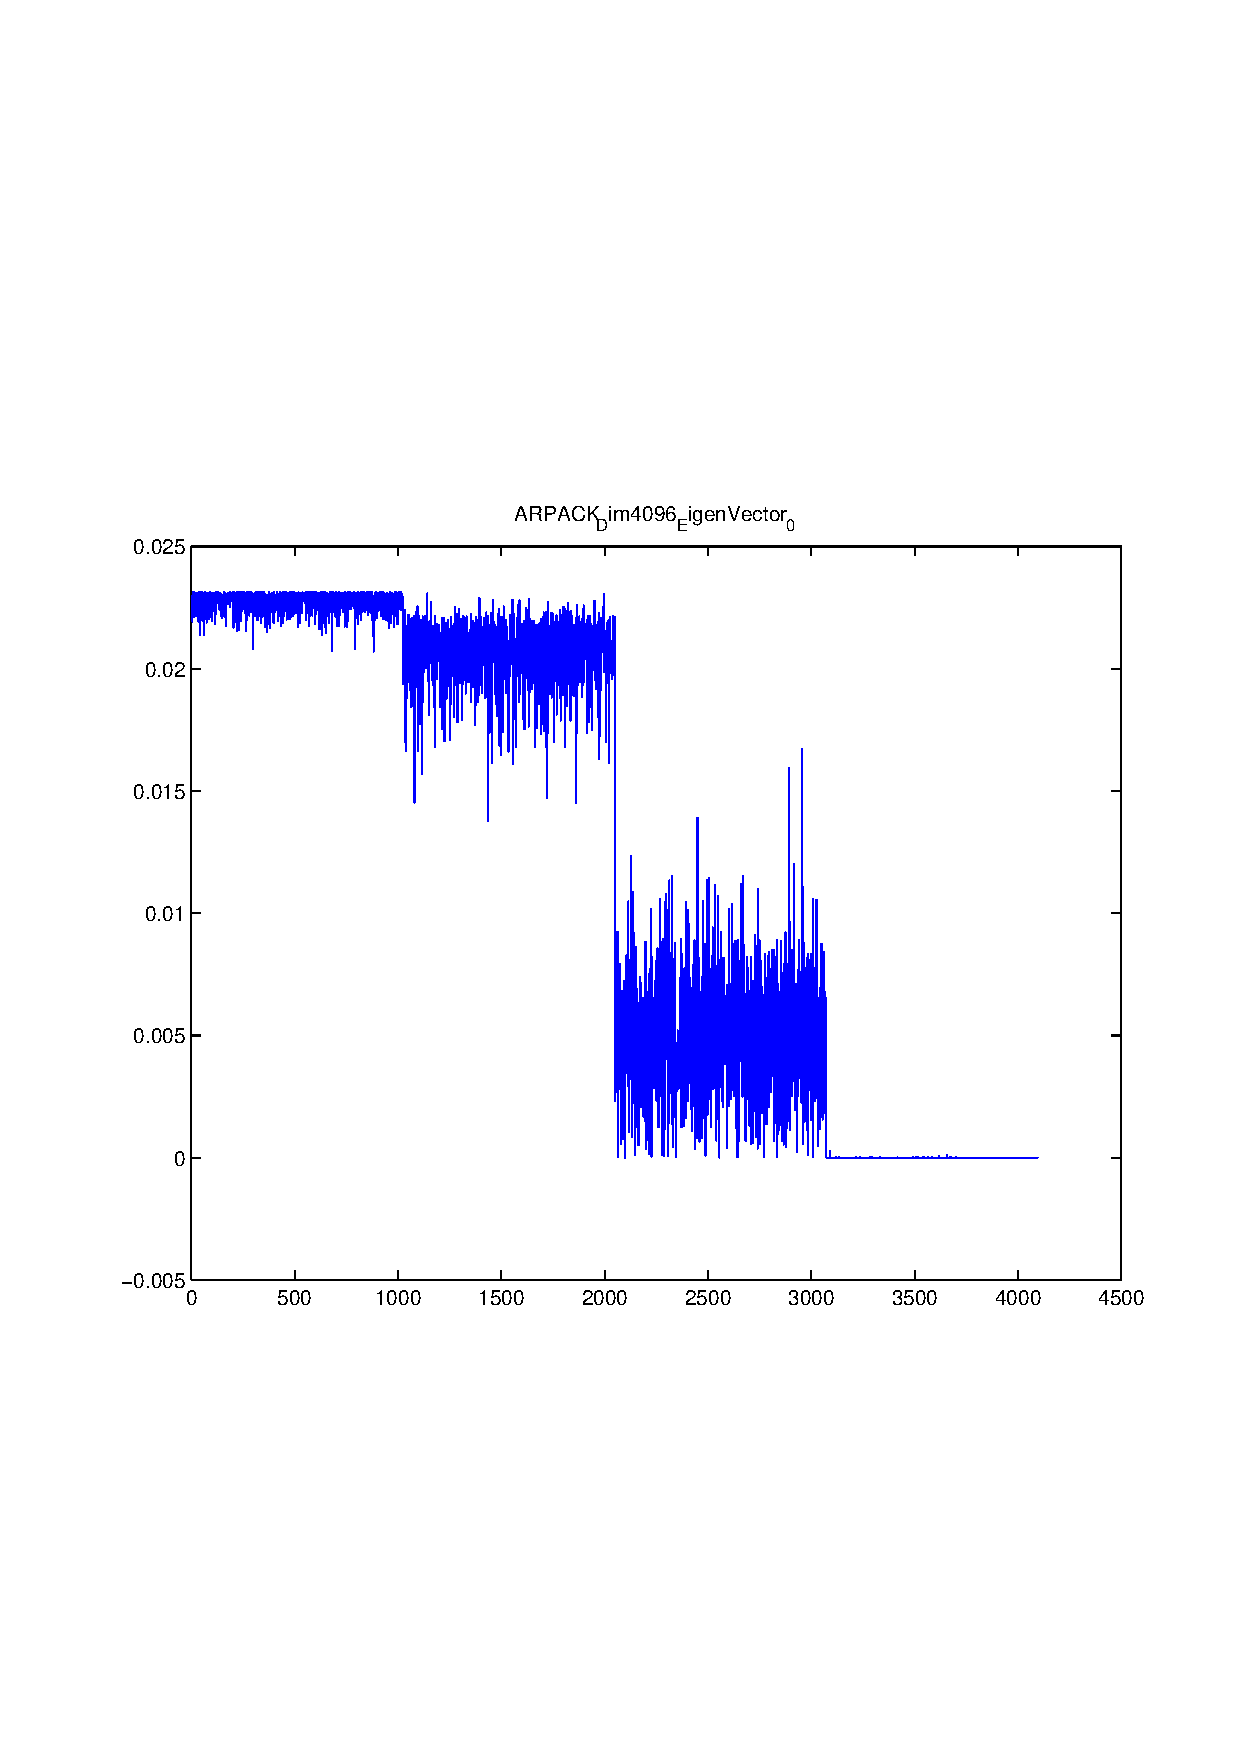
\includegraphics[width=10.0cm,height=10.0cm]{ARPACK_Dim4096_EigenVector_0.pdf}

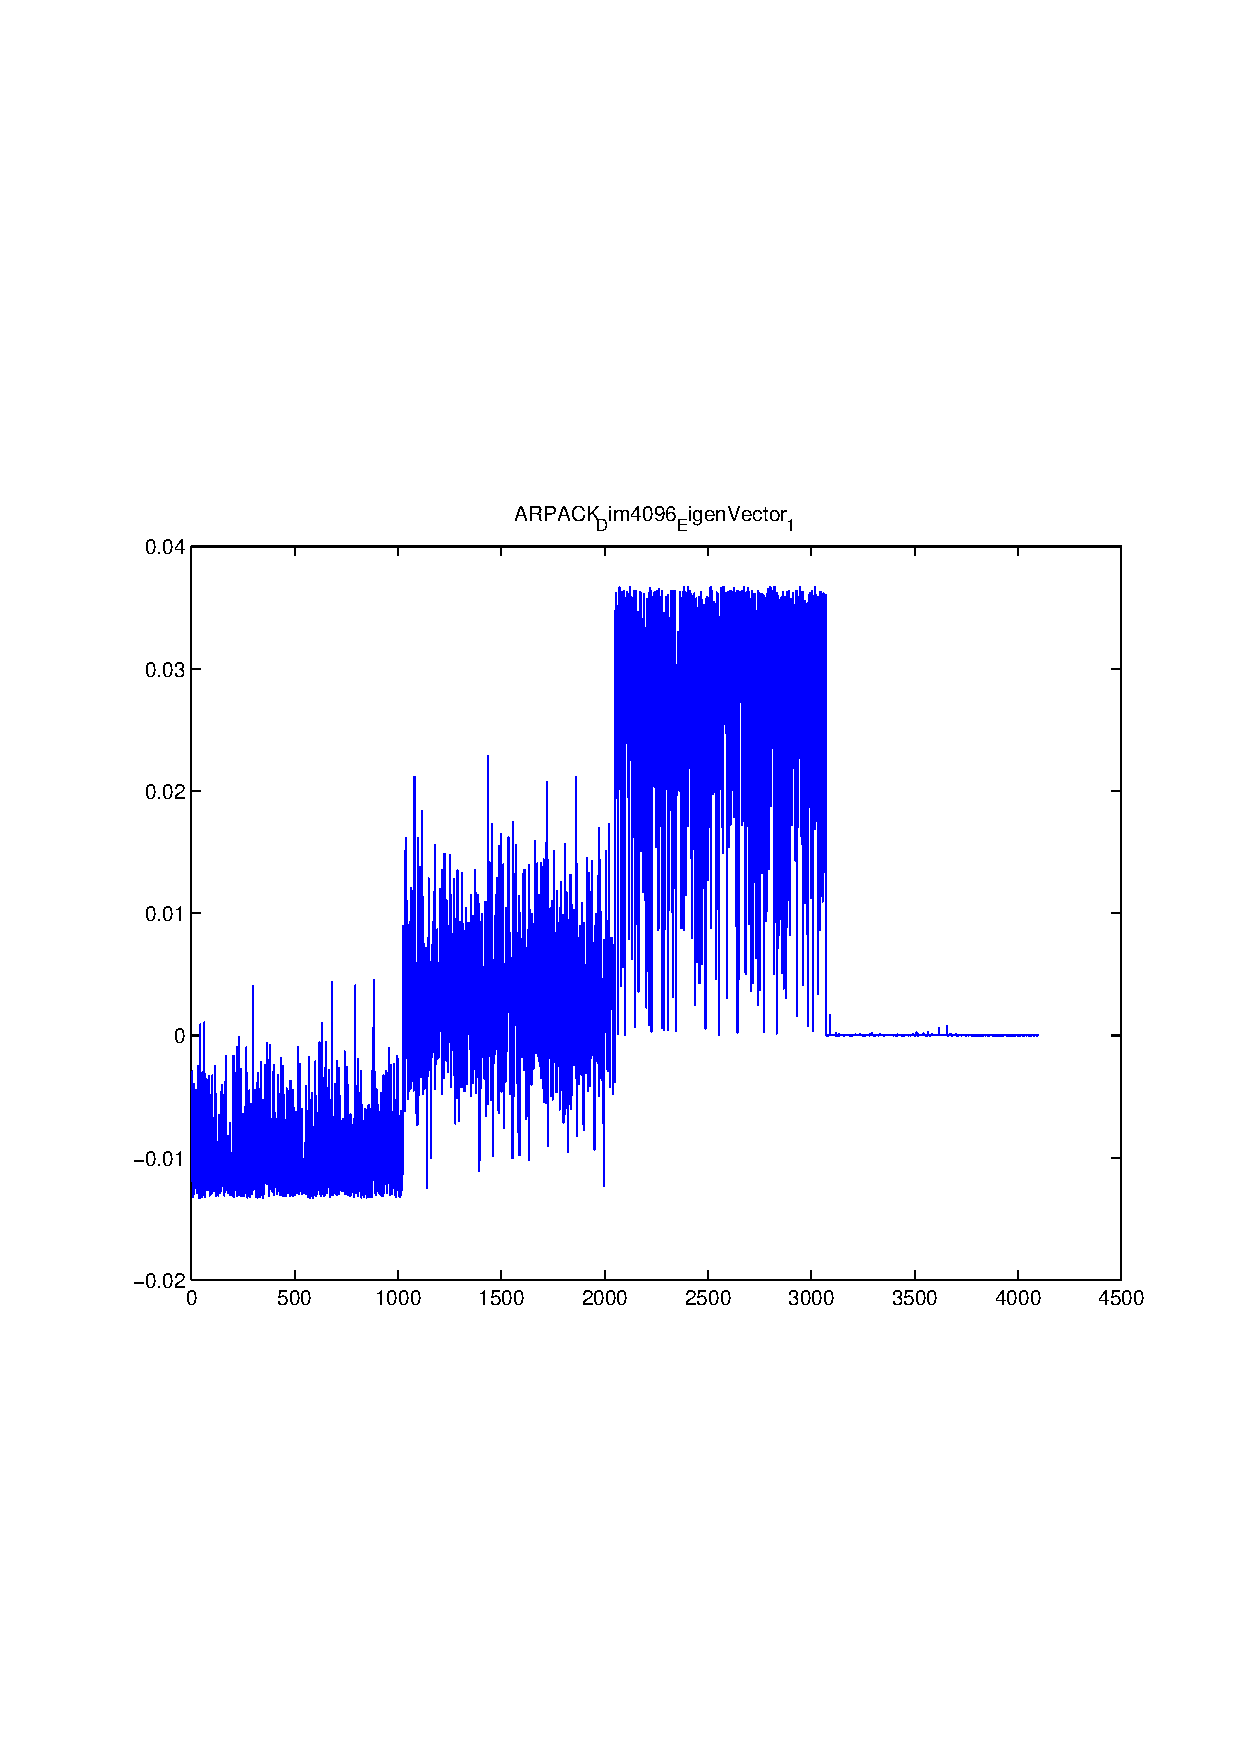
\includegraphics[width=10.0cm,height=10.0cm]{ARPACK_Dim4096_EigenVector_1.pdf}

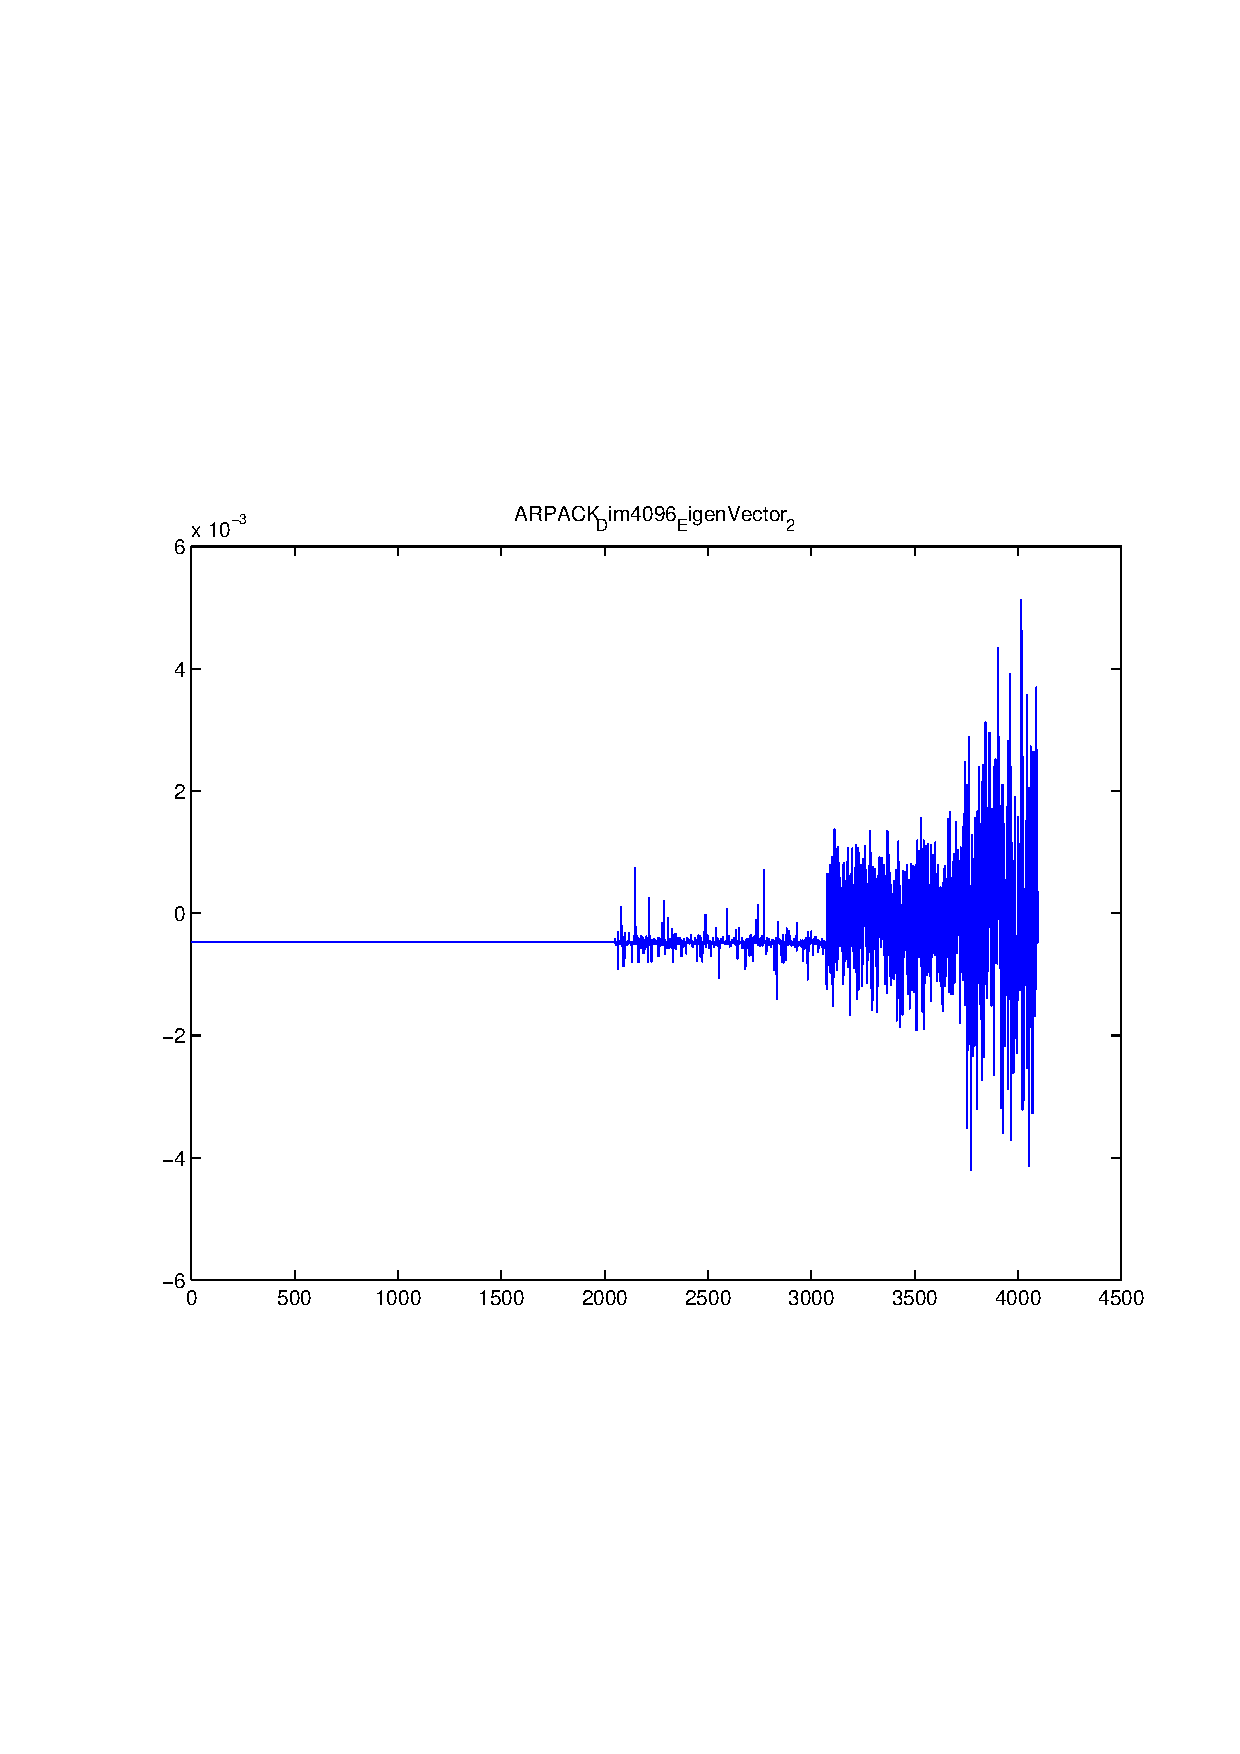
\includegraphics[width=10.0cm,height=10.0cm]{ARPACK_Dim4096_EigenVector_2.pdf}

\includegraphics[width=10.0cm,height=10.0cm]{ARPACK_Dim4096_EigenVector_3.pdf}

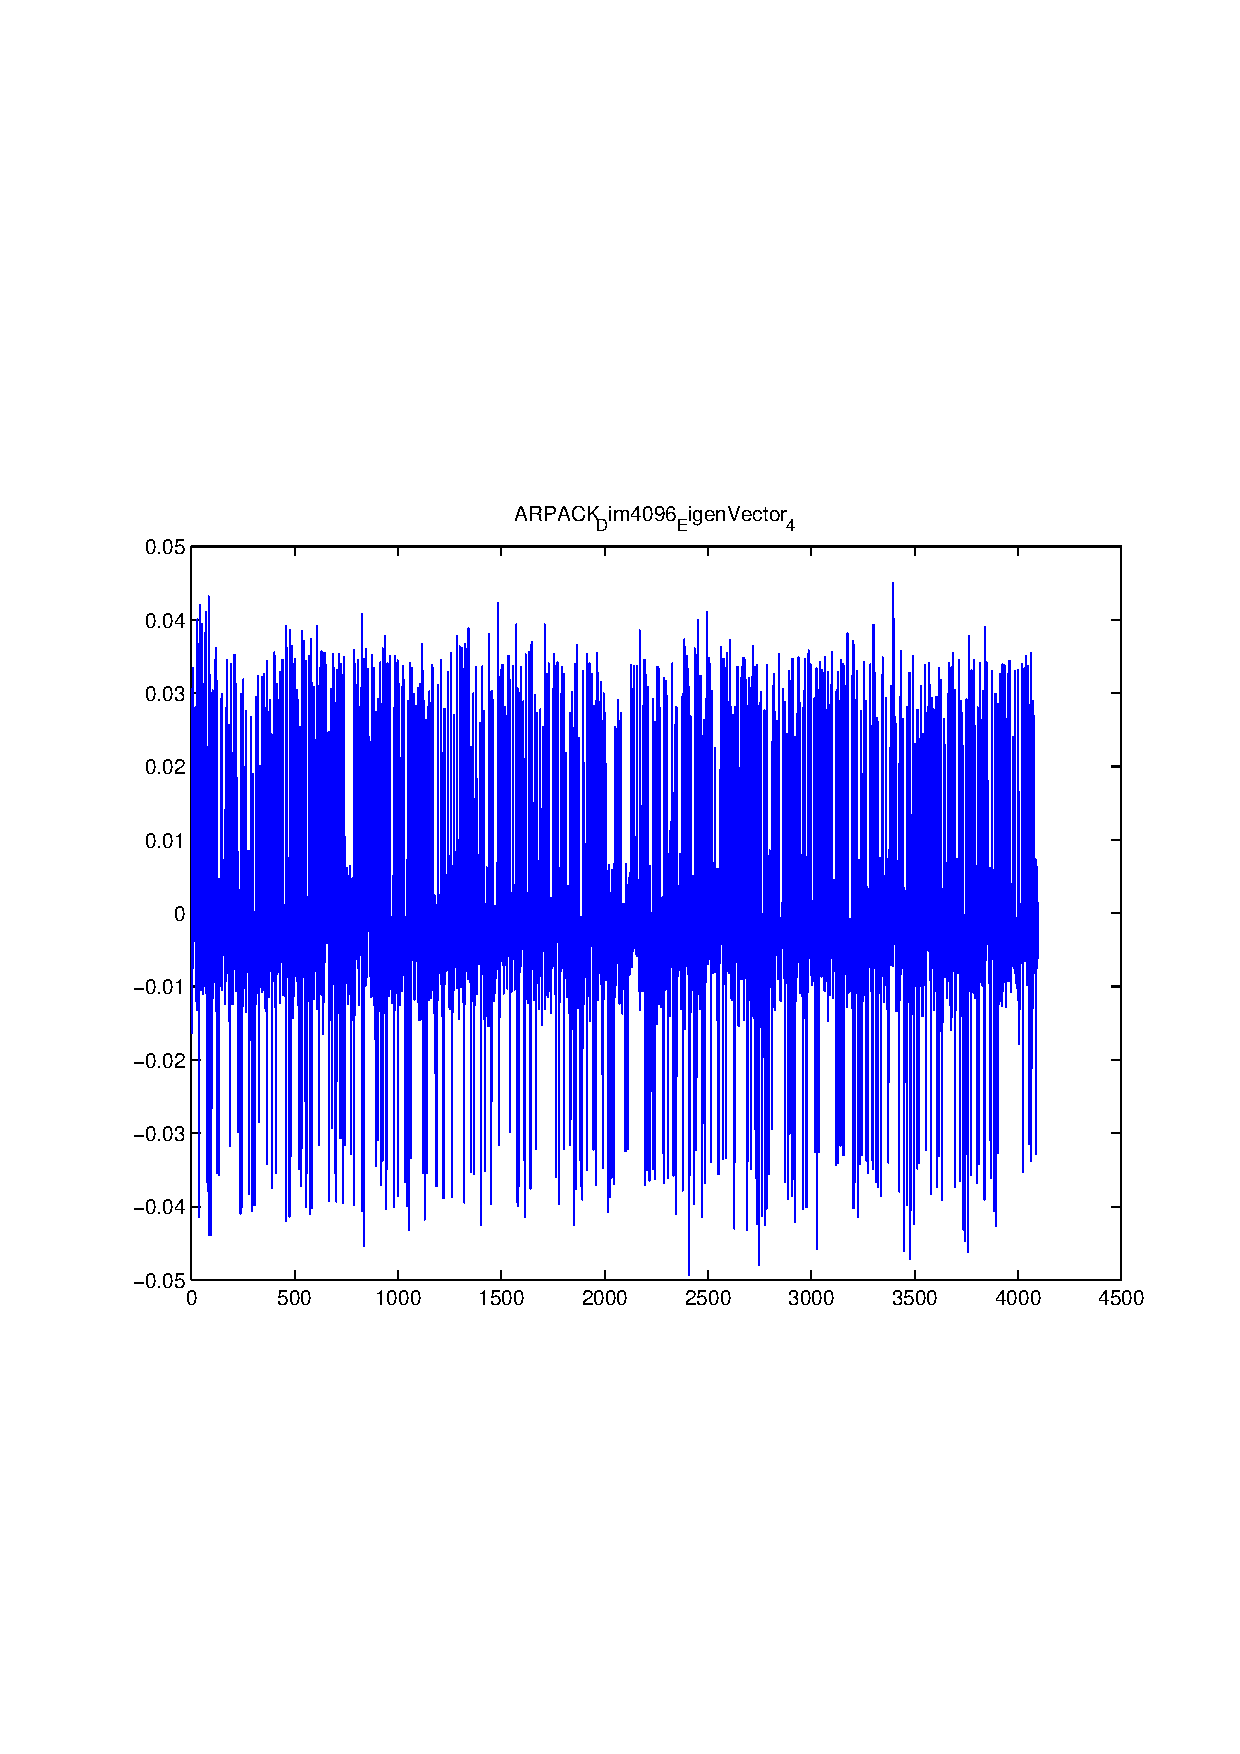
\includegraphics[width=10.0cm,height=10.0cm]{ARPACK_Dim4096_EigenVector_4.pdf}

Iterative Krylov dim=4096 dt=10.7756
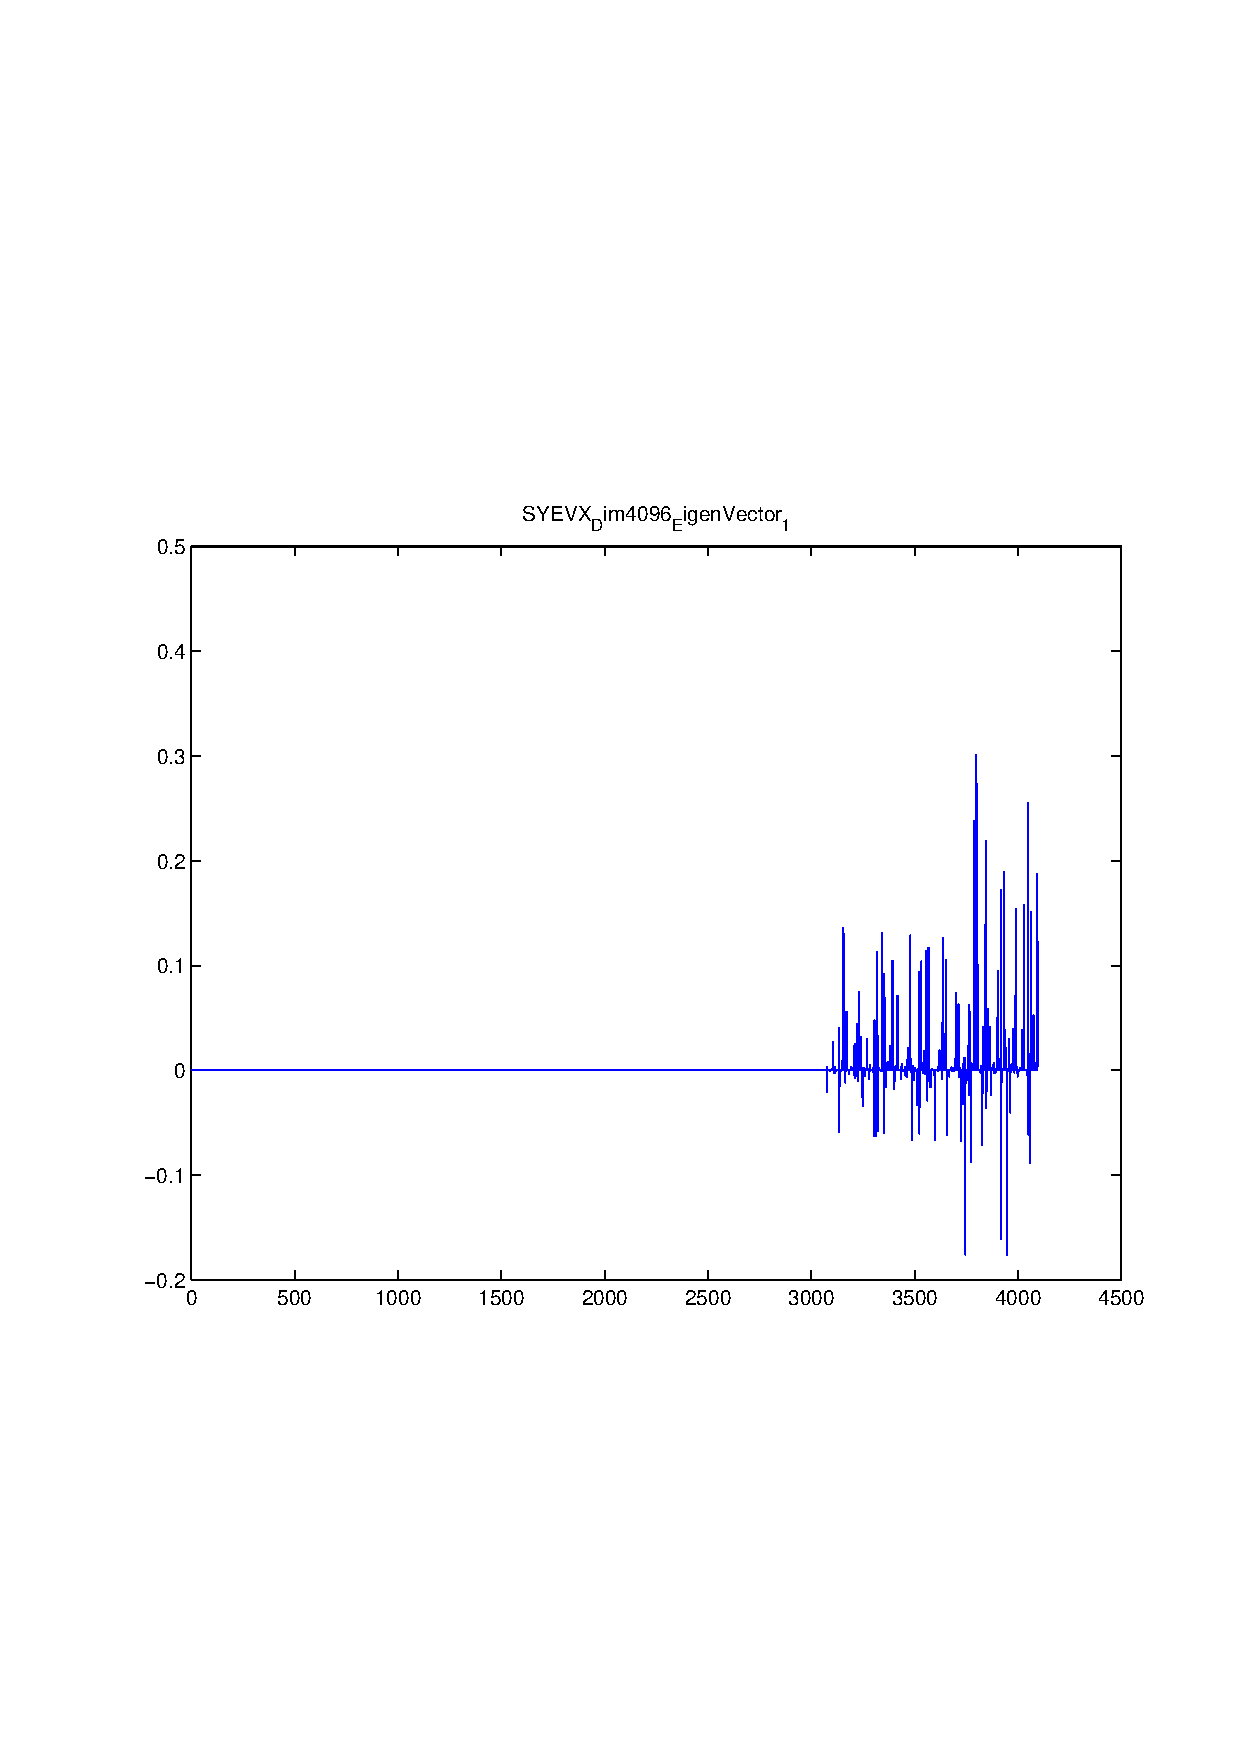
\includegraphics[width=10.0cm,height=10.0cm]{SYEVX_Dim4096_EigenVector_1.pdf}

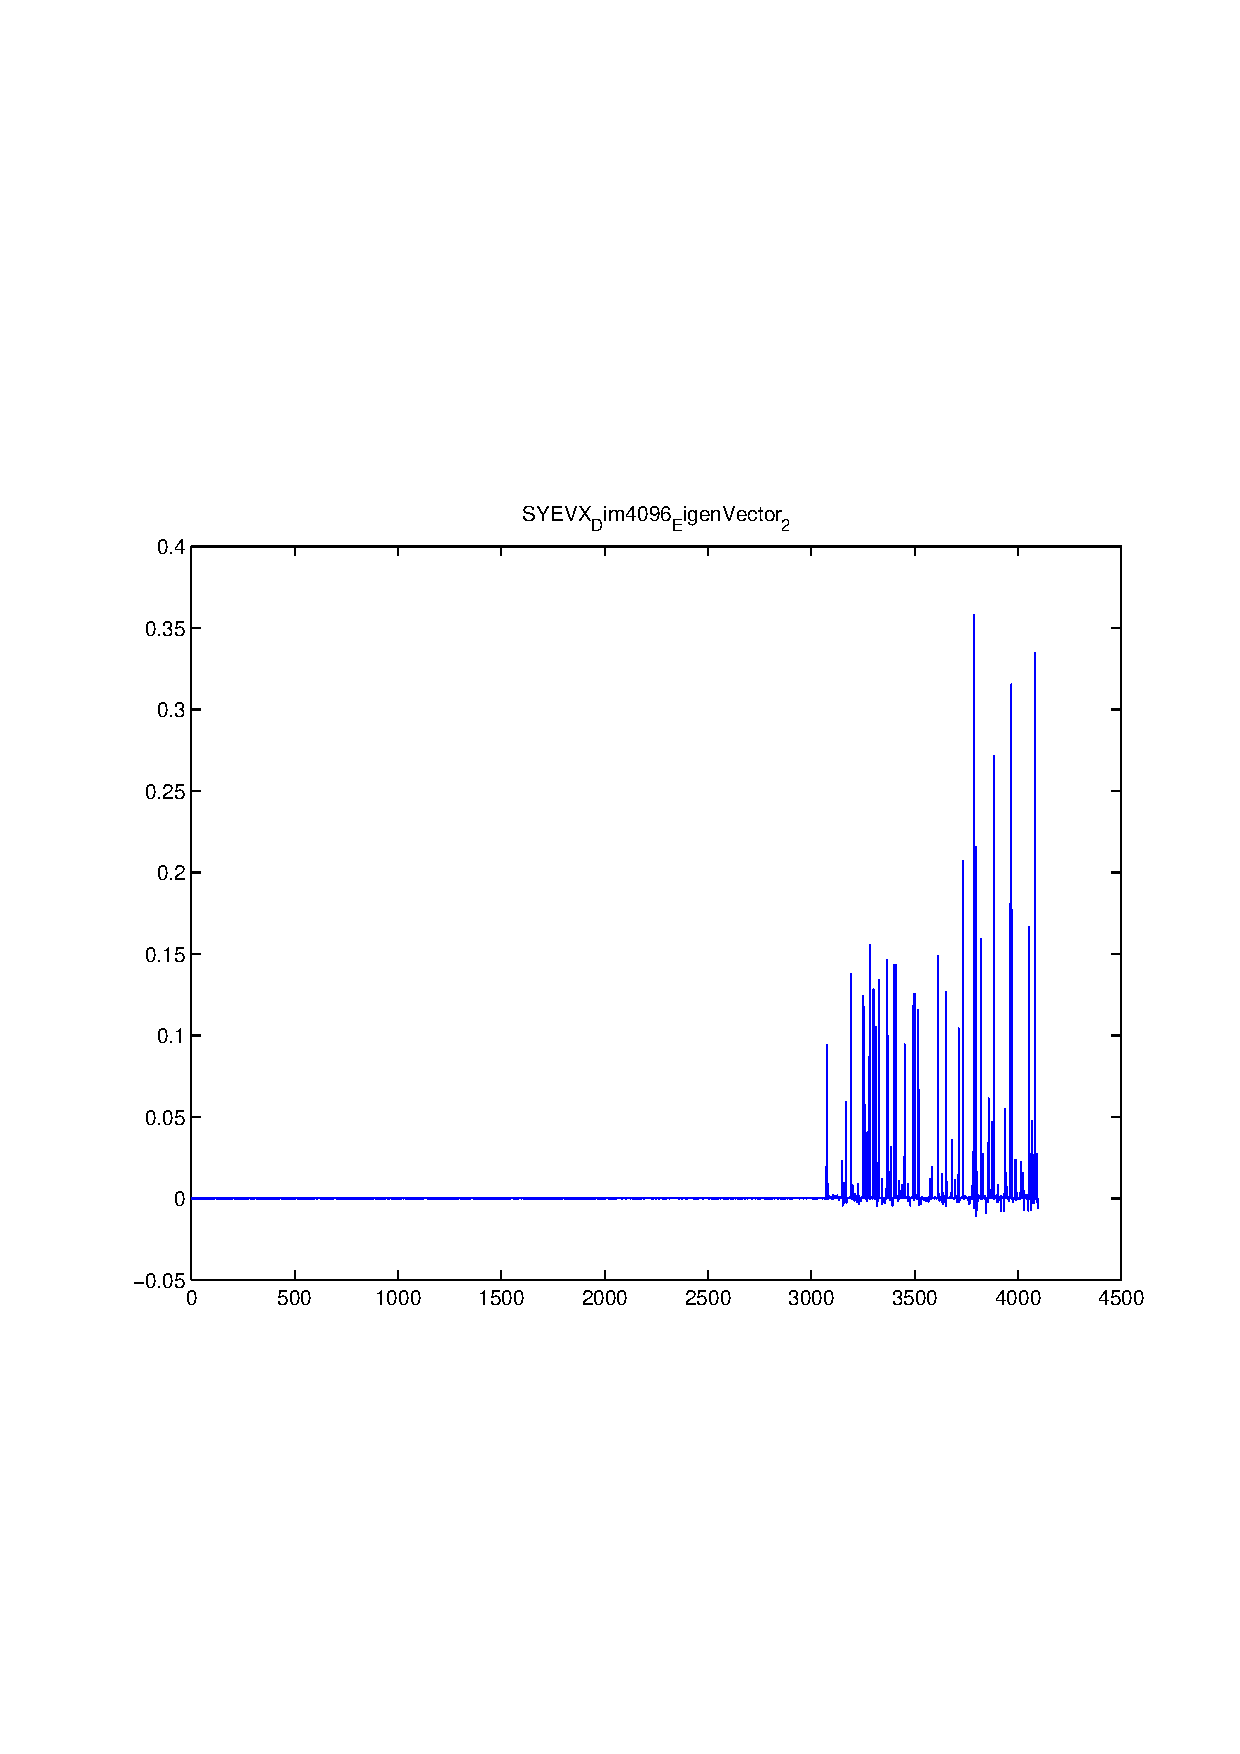
\includegraphics[width=10.0cm,height=10.0cm]{SYEVX_Dim4096_EigenVector_2.pdf}

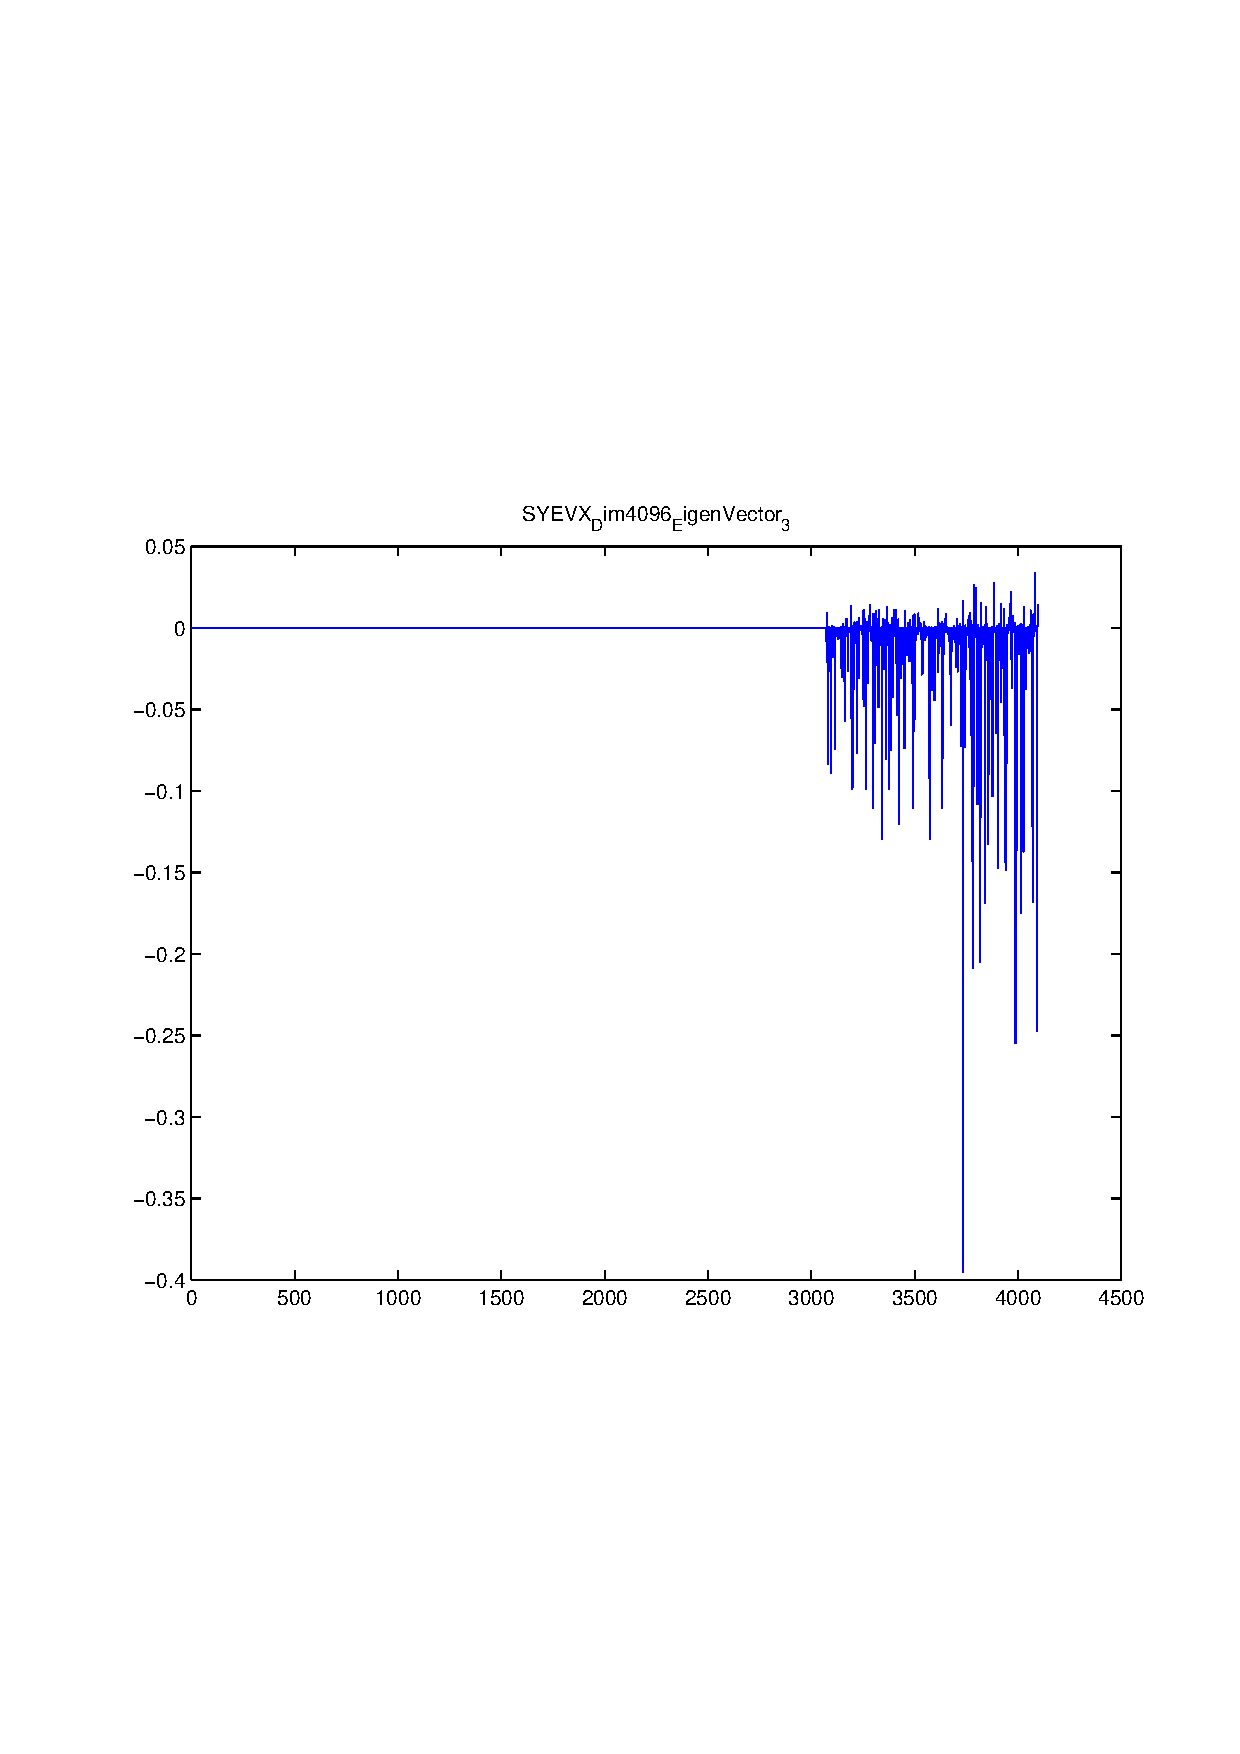
\includegraphics[width=10.0cm,height=10.0cm]{SYEVX_Dim4096_EigenVector_3.pdf}

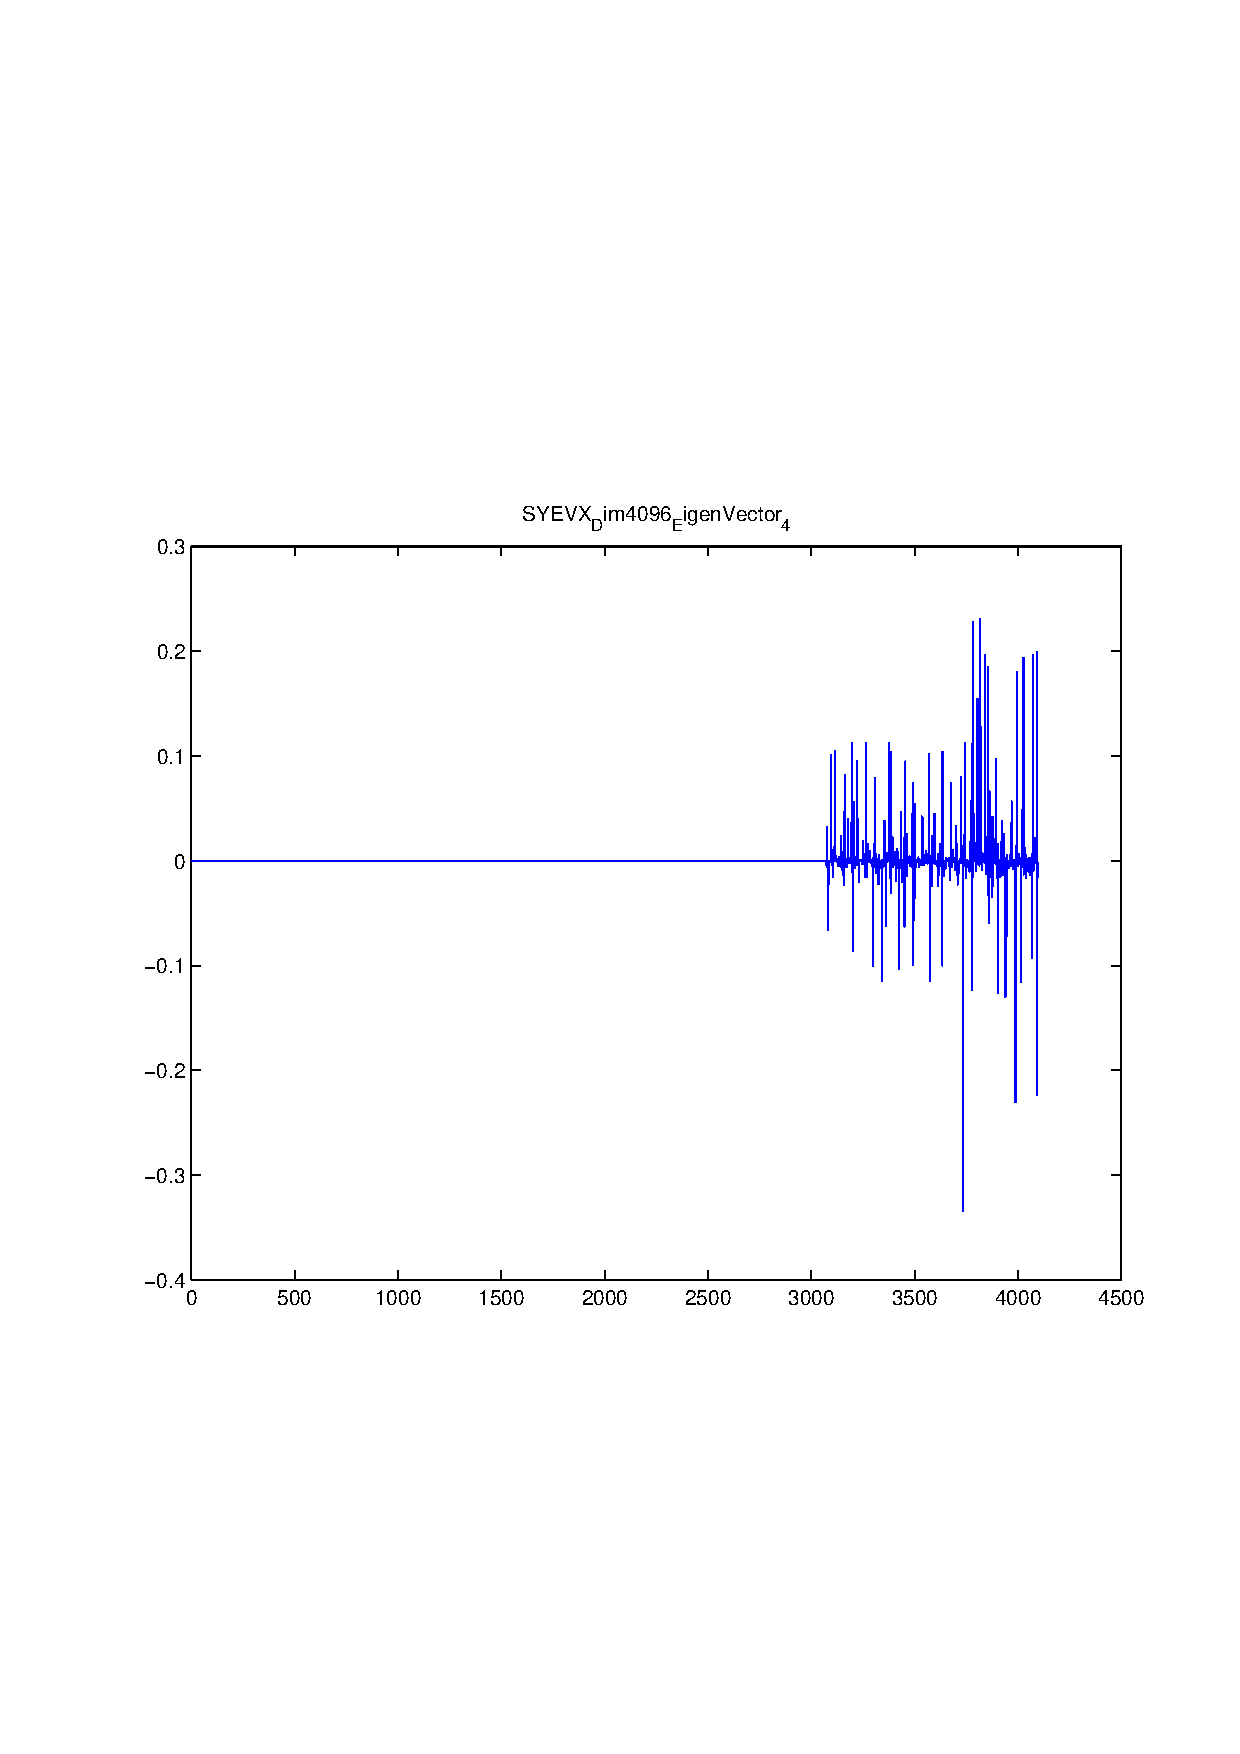
\includegraphics[width=10.0cm,height=10.0cm]{SYEVX_Dim4096_EigenVector_4.pdf}

tic toc fileistream read dim n=4608 dt=238.657
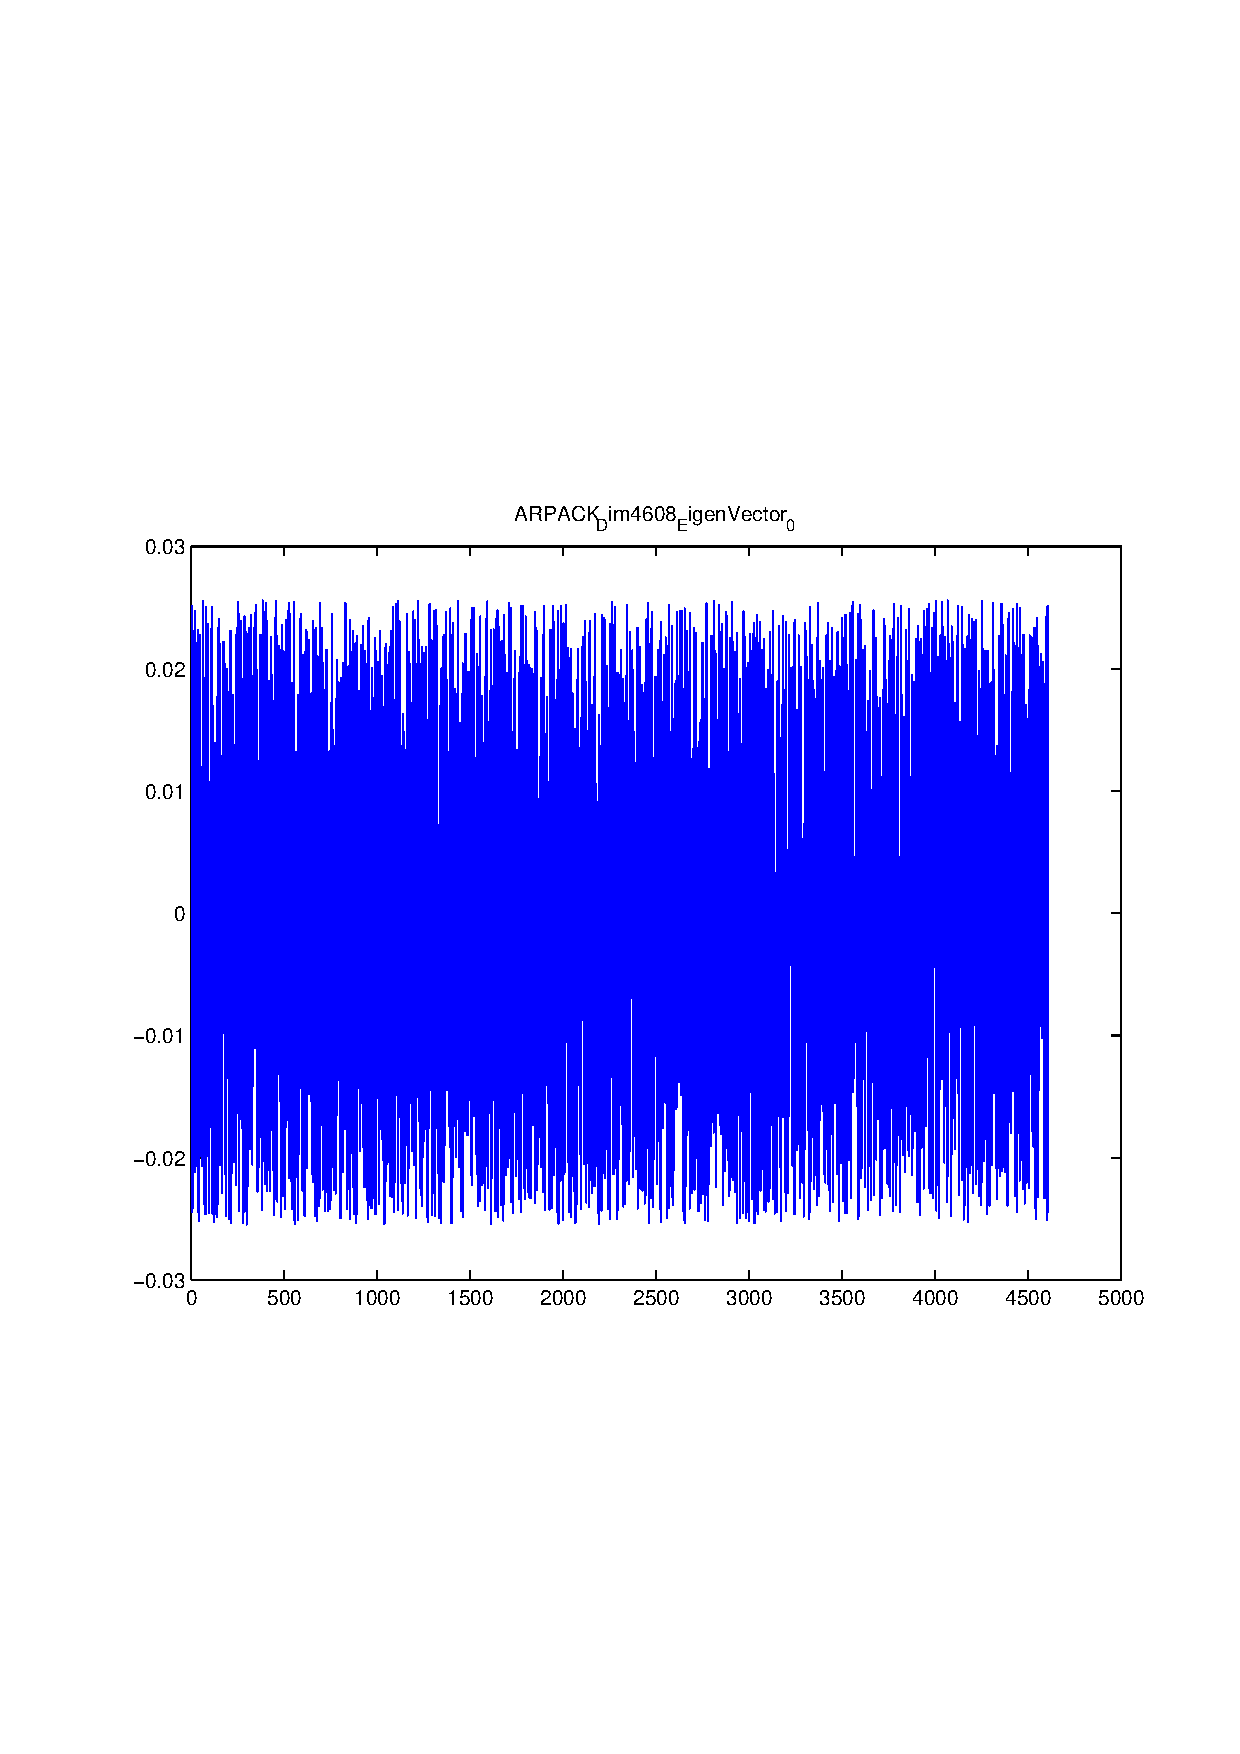
\includegraphics[width=10.0cm,height=10.0cm]{ARPACK_Dim4608_EigenVector_0.pdf}

\includegraphics[width=10.0cm,height=10.0cm]{ARPACK_Dim4608_EigenVector_1.pdf}

\includegraphics[width=10.0cm,height=10.0cm]{ARPACK_Dim4608_EigenVector_2.pdf}

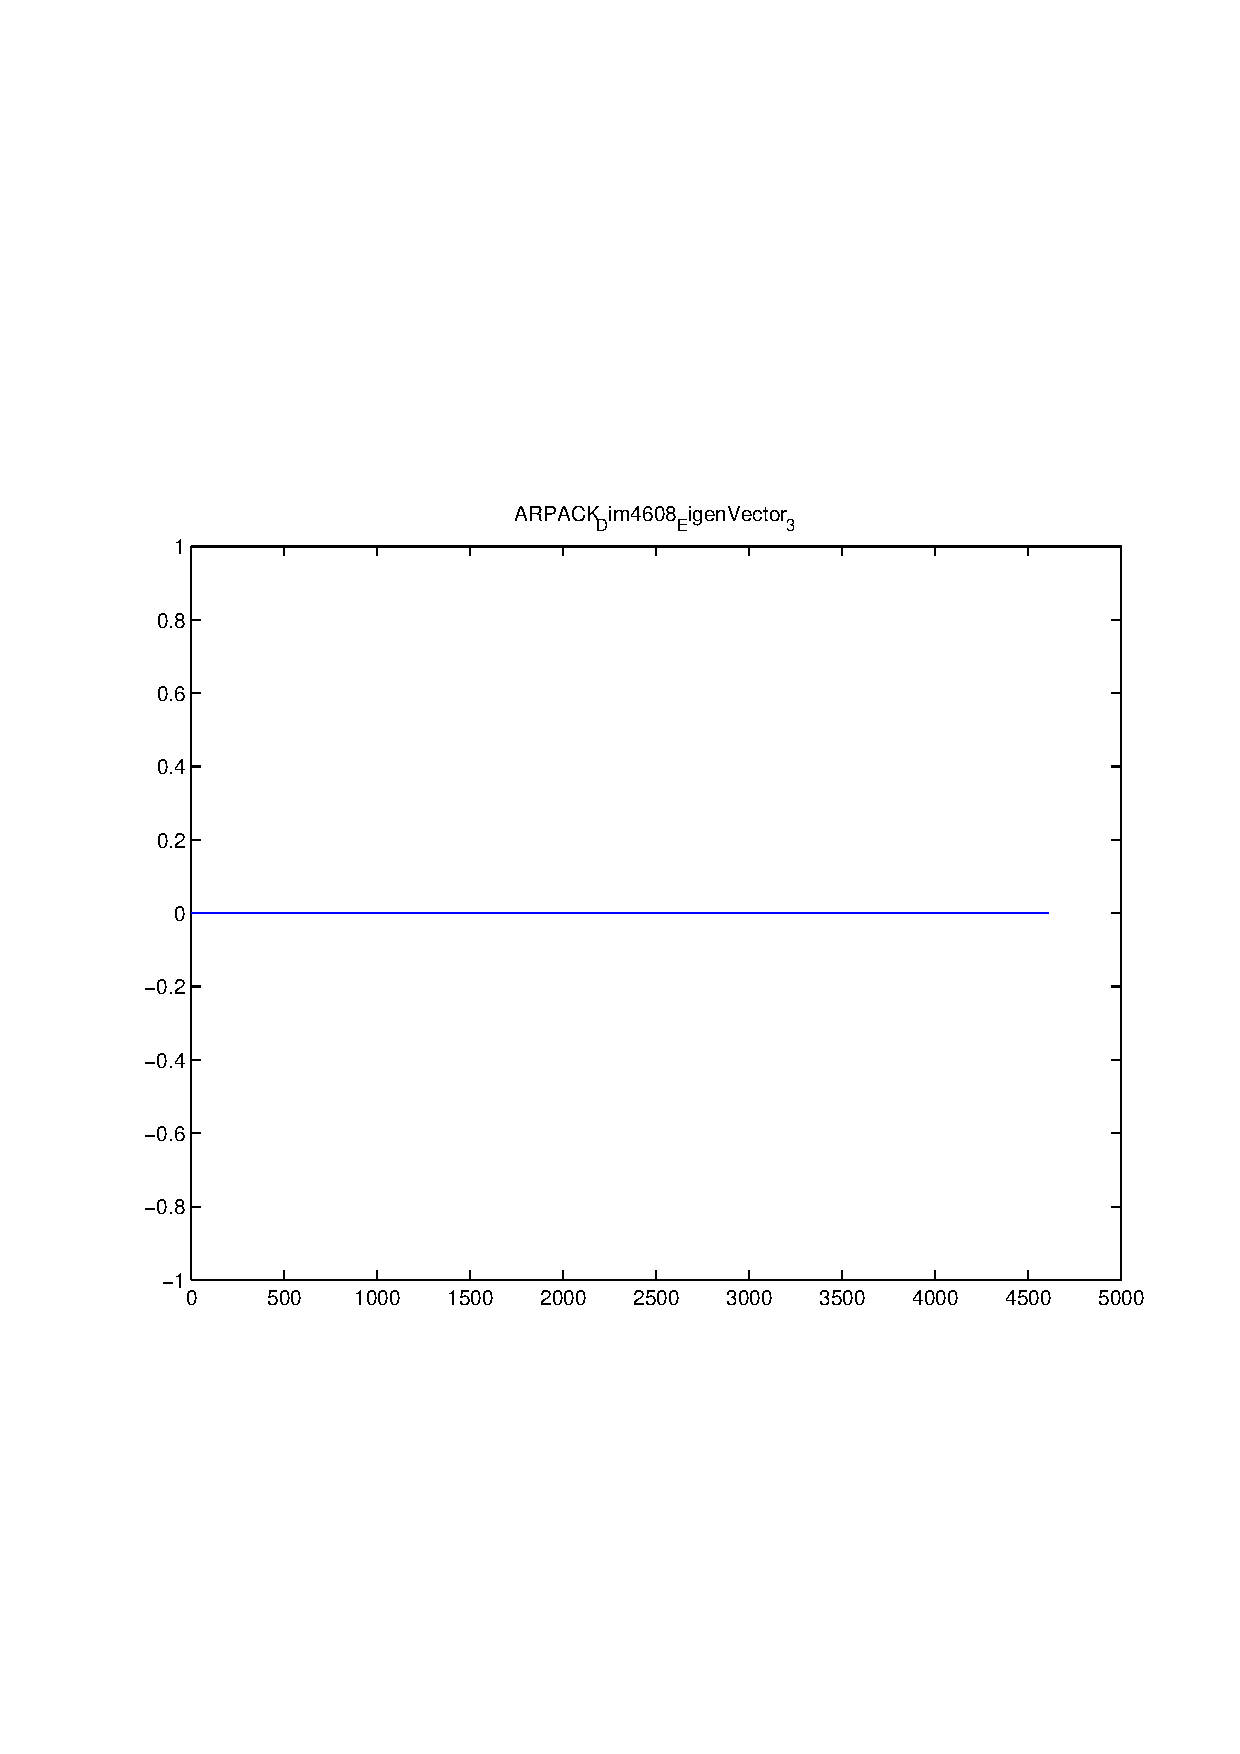
\includegraphics[width=10.0cm,height=10.0cm]{ARPACK_Dim4608_EigenVector_3.pdf}

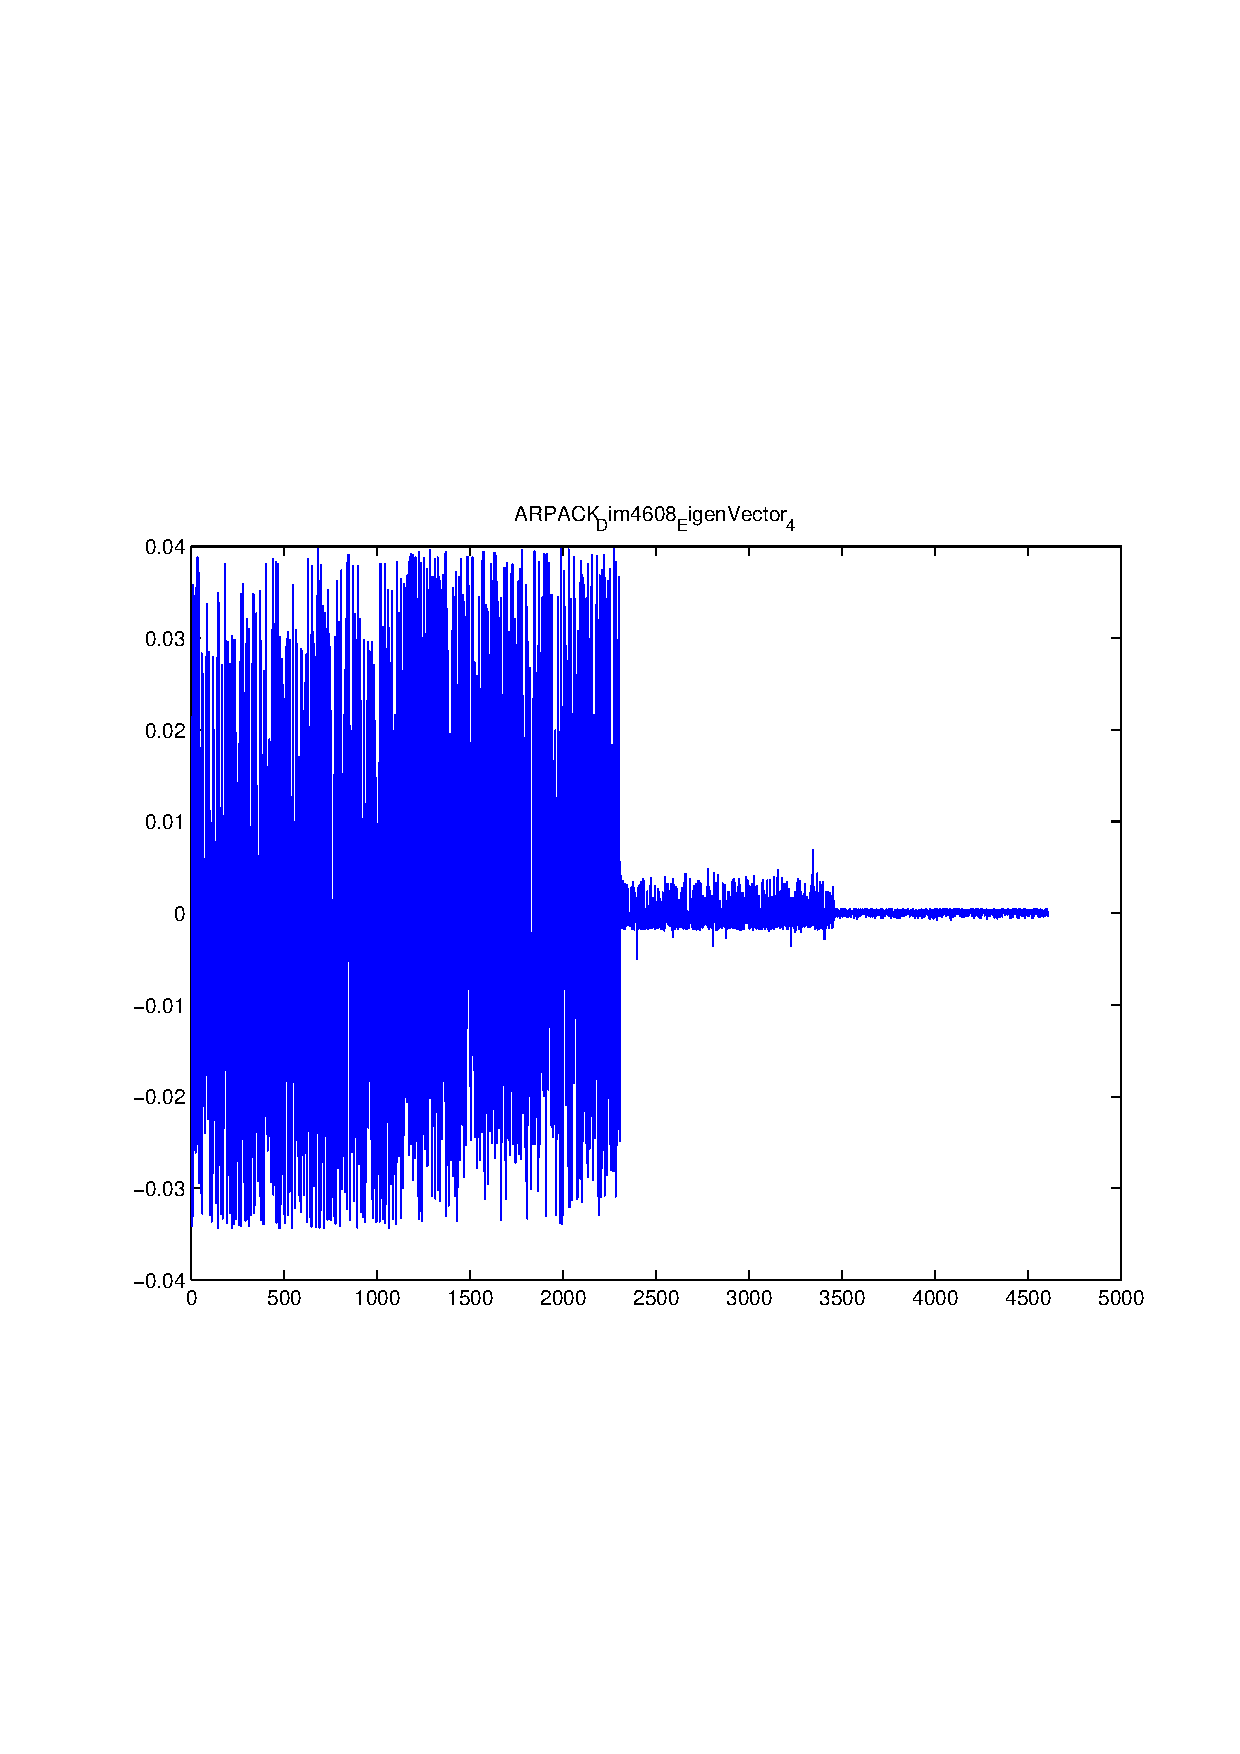
\includegraphics[width=10.0cm,height=10.0cm]{ARPACK_Dim4608_EigenVector_4.pdf}

Iterative Krylov dim=4608 dt=12.1255
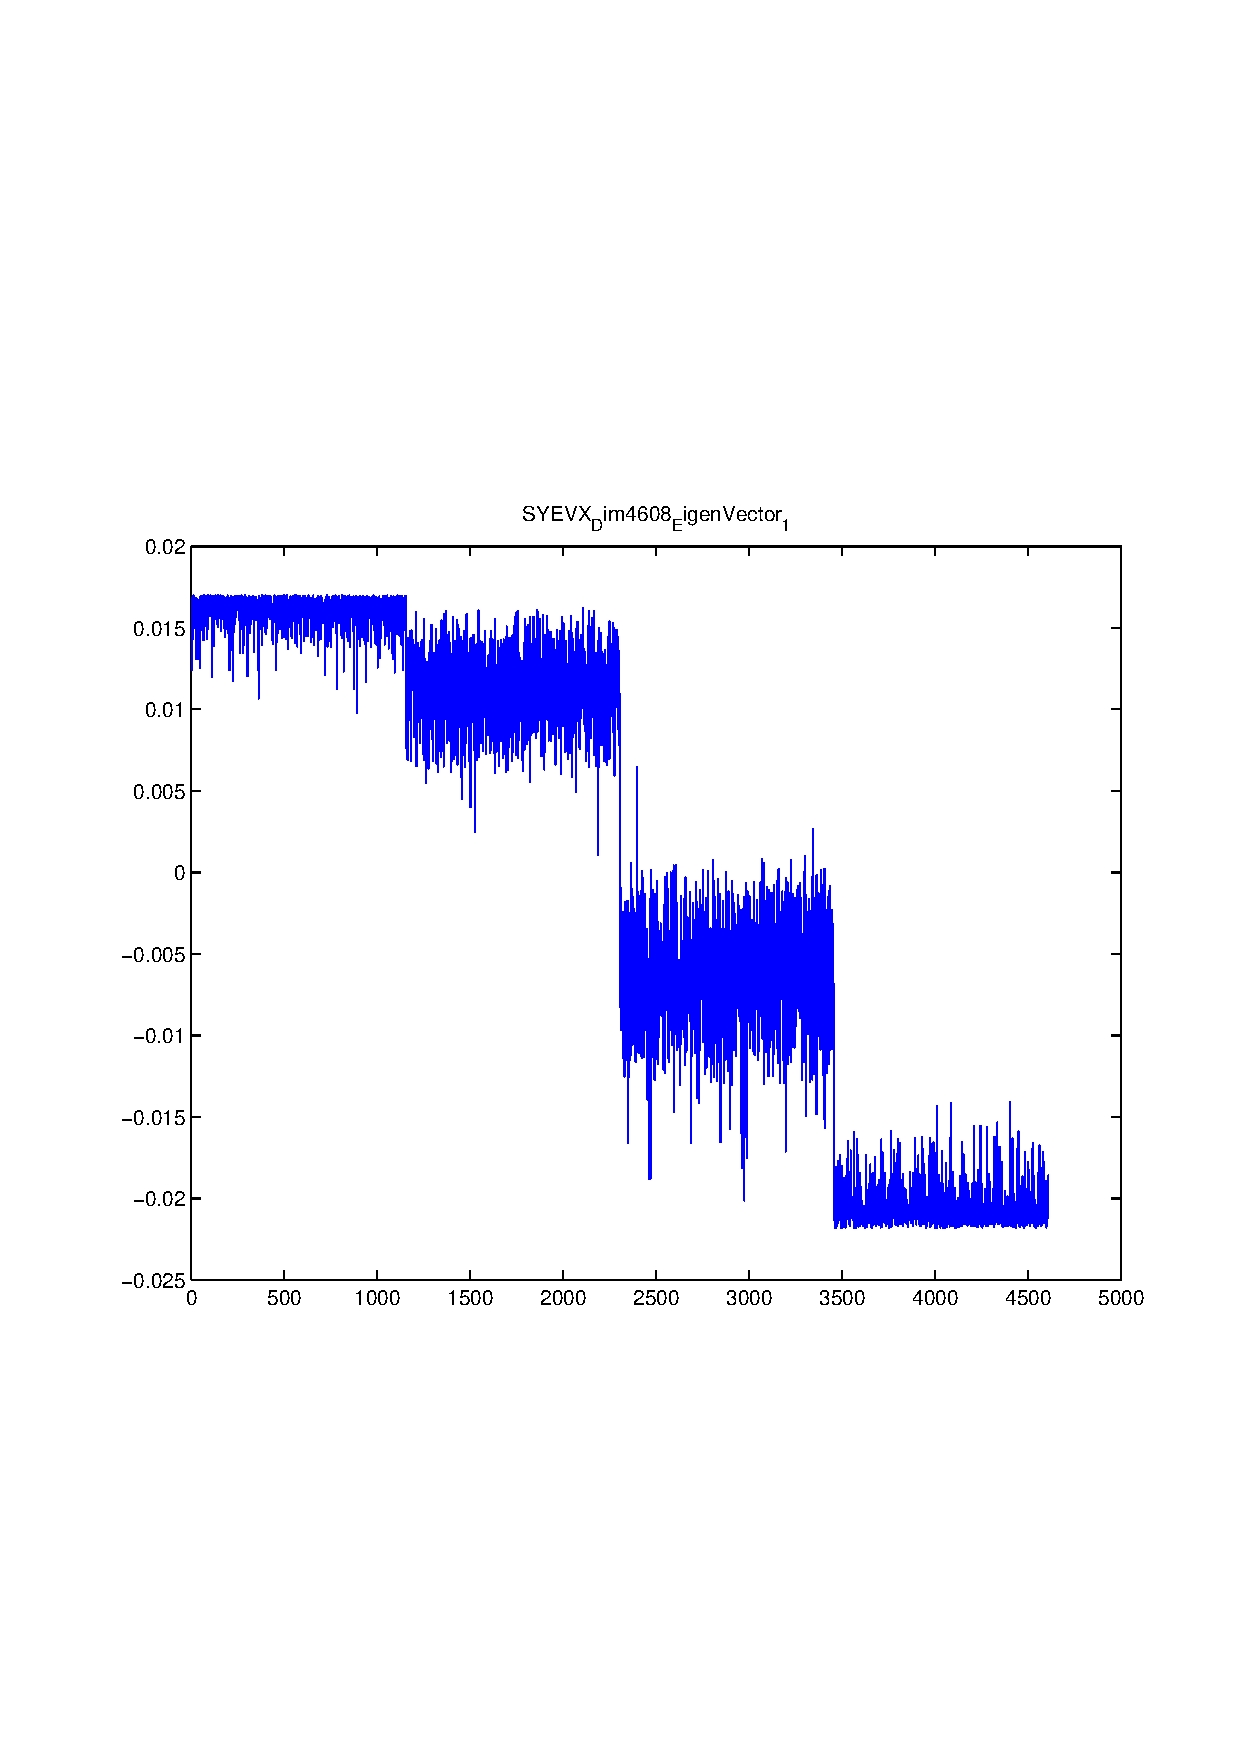
\includegraphics[width=10.0cm,height=10.0cm]{SYEVX_Dim4608_EigenVector_1.pdf}

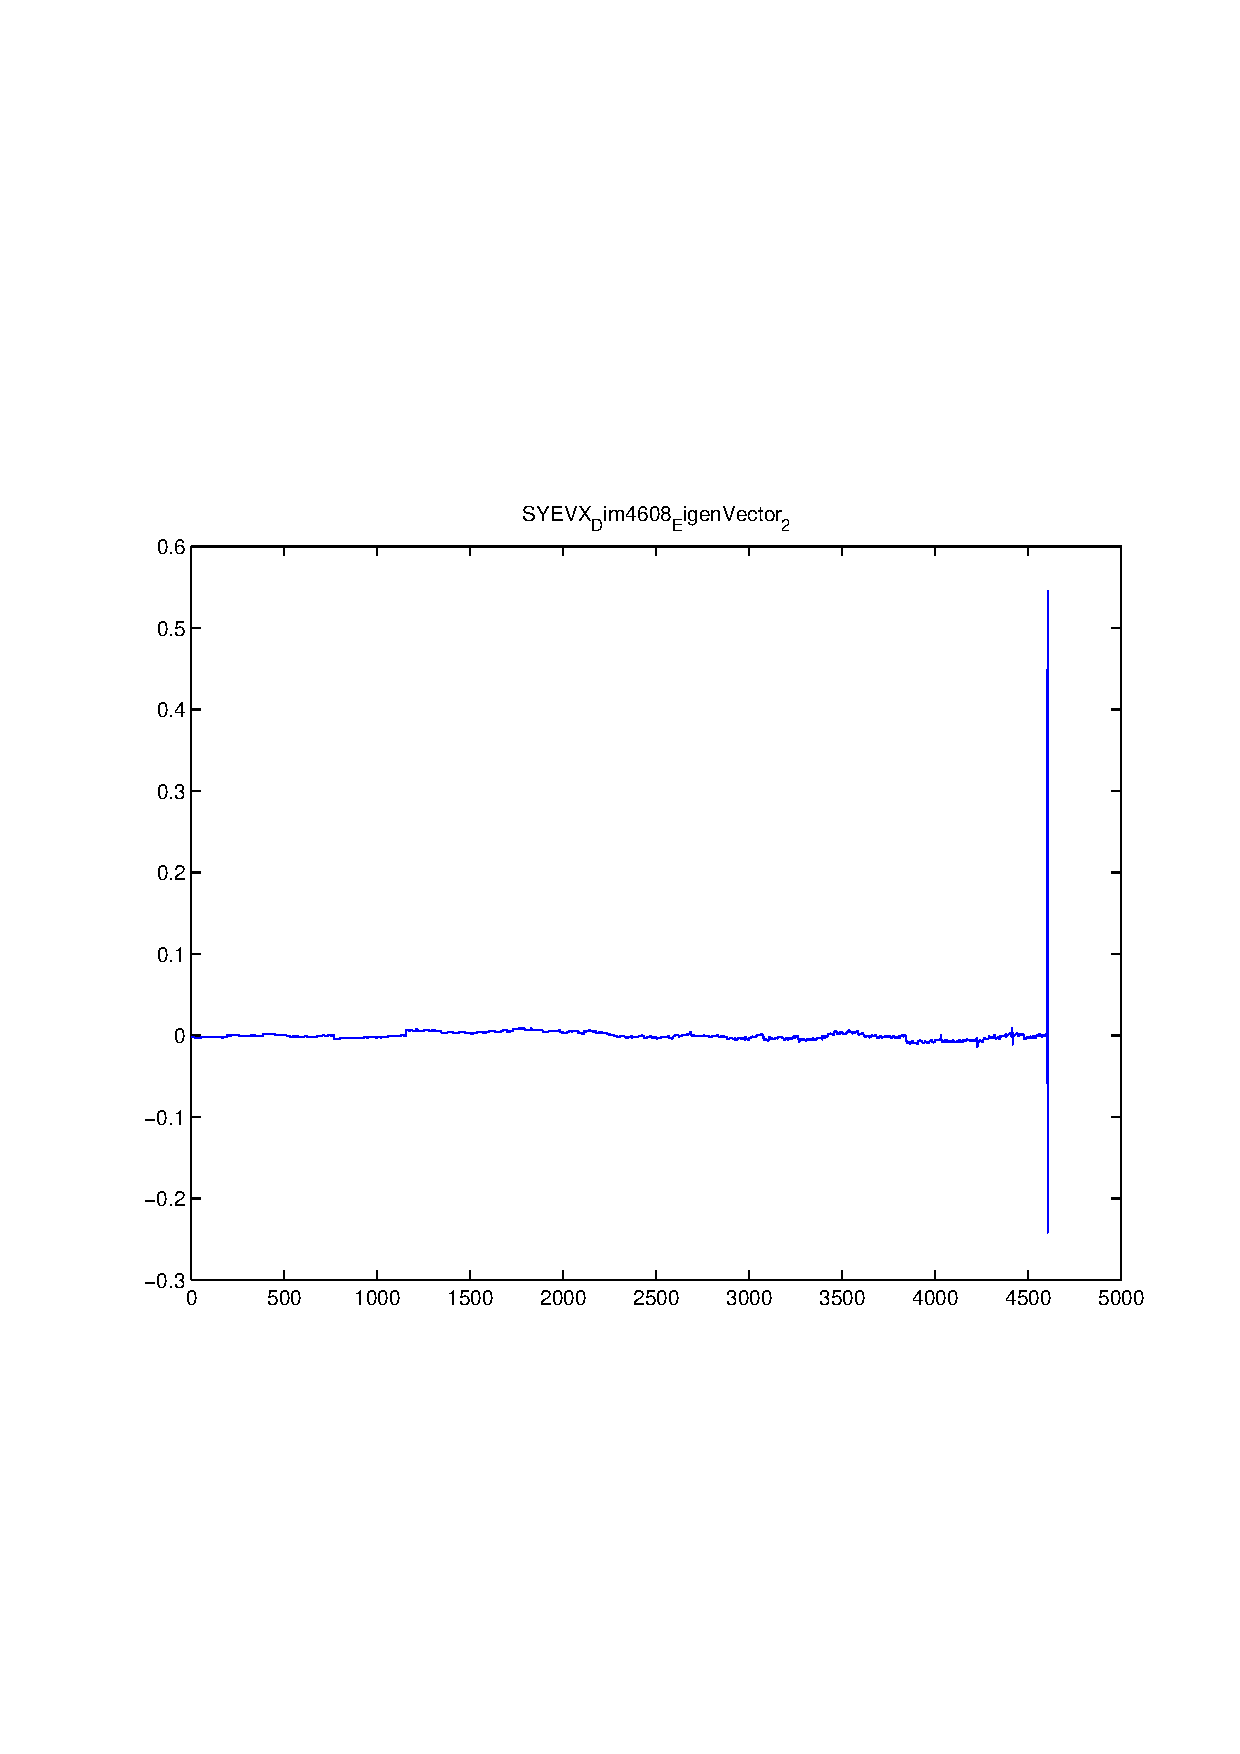
\includegraphics[width=10.0cm,height=10.0cm]{SYEVX_Dim4608_EigenVector_2.pdf}

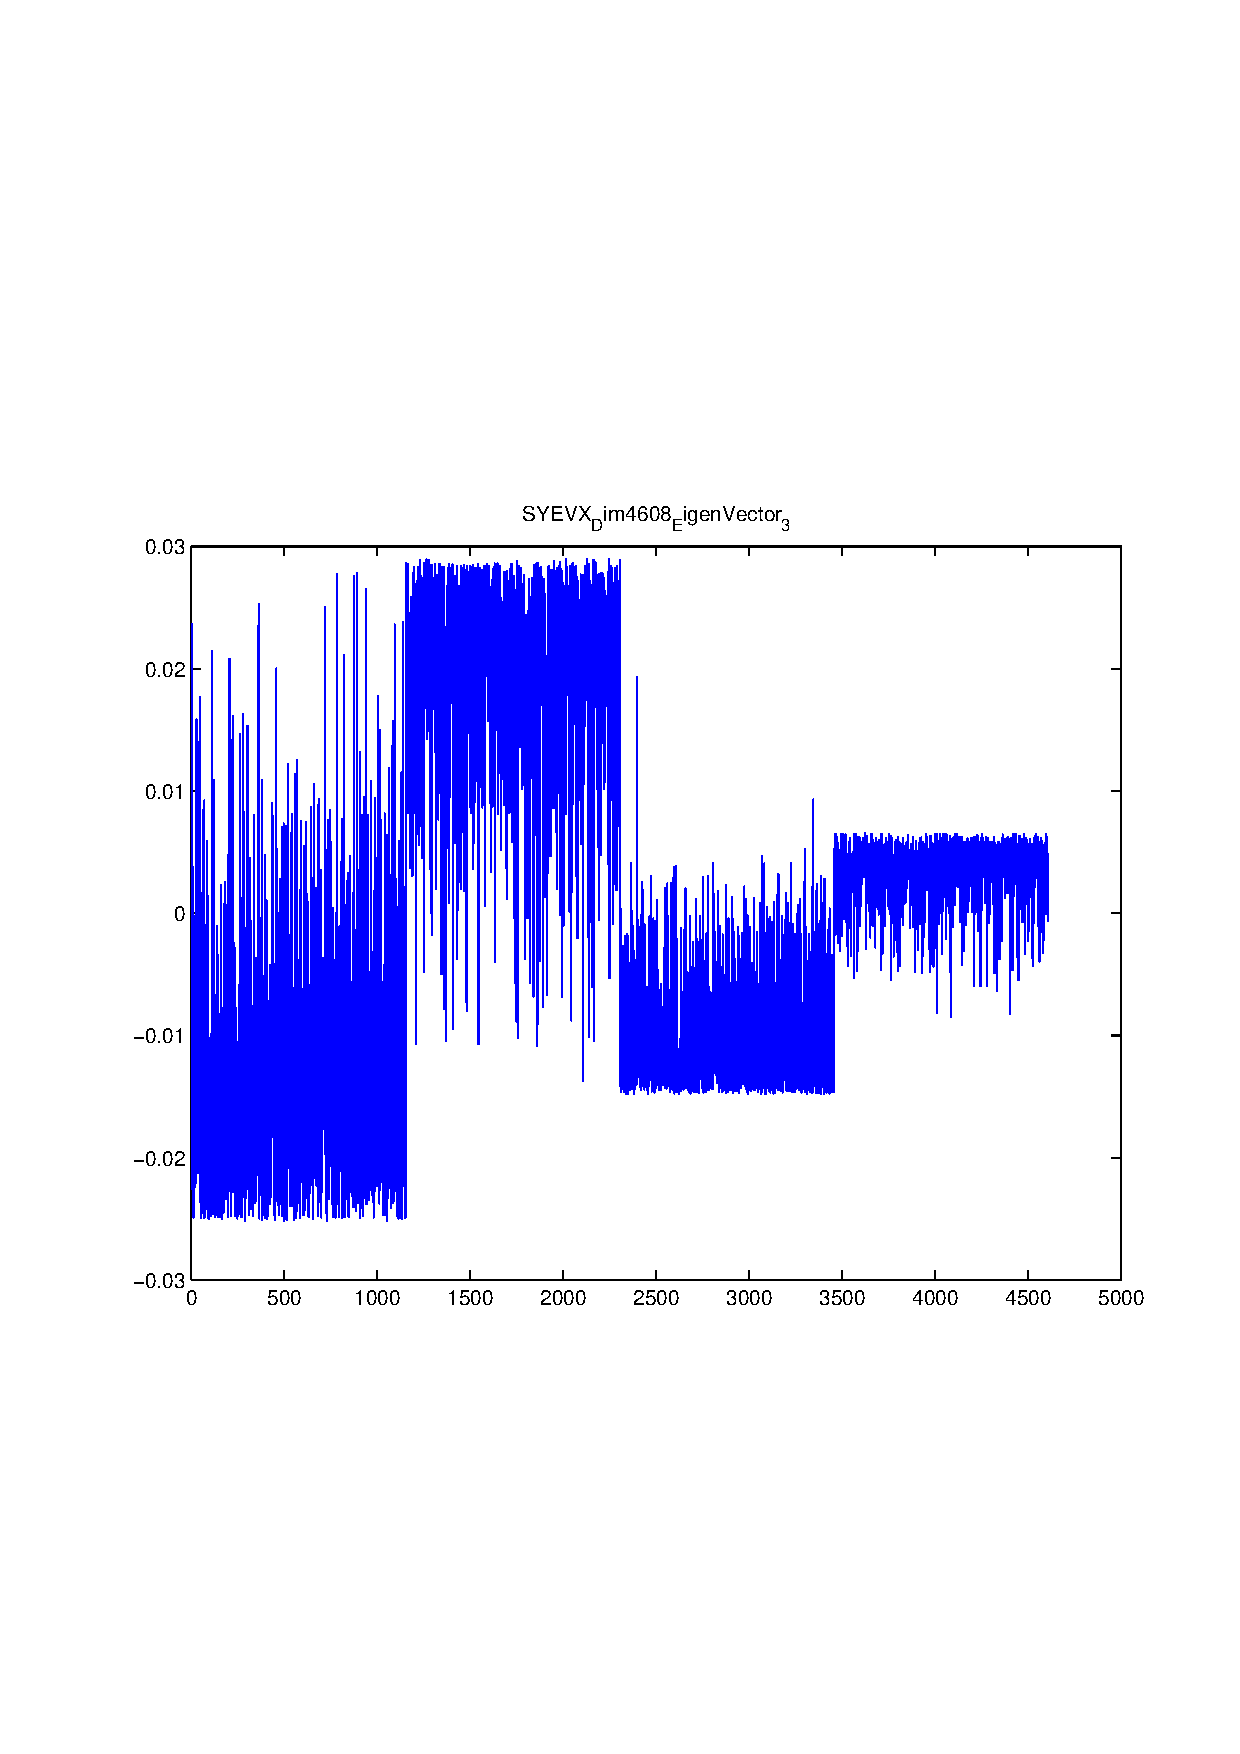
\includegraphics[width=10.0cm,height=10.0cm]{SYEVX_Dim4608_EigenVector_3.pdf}

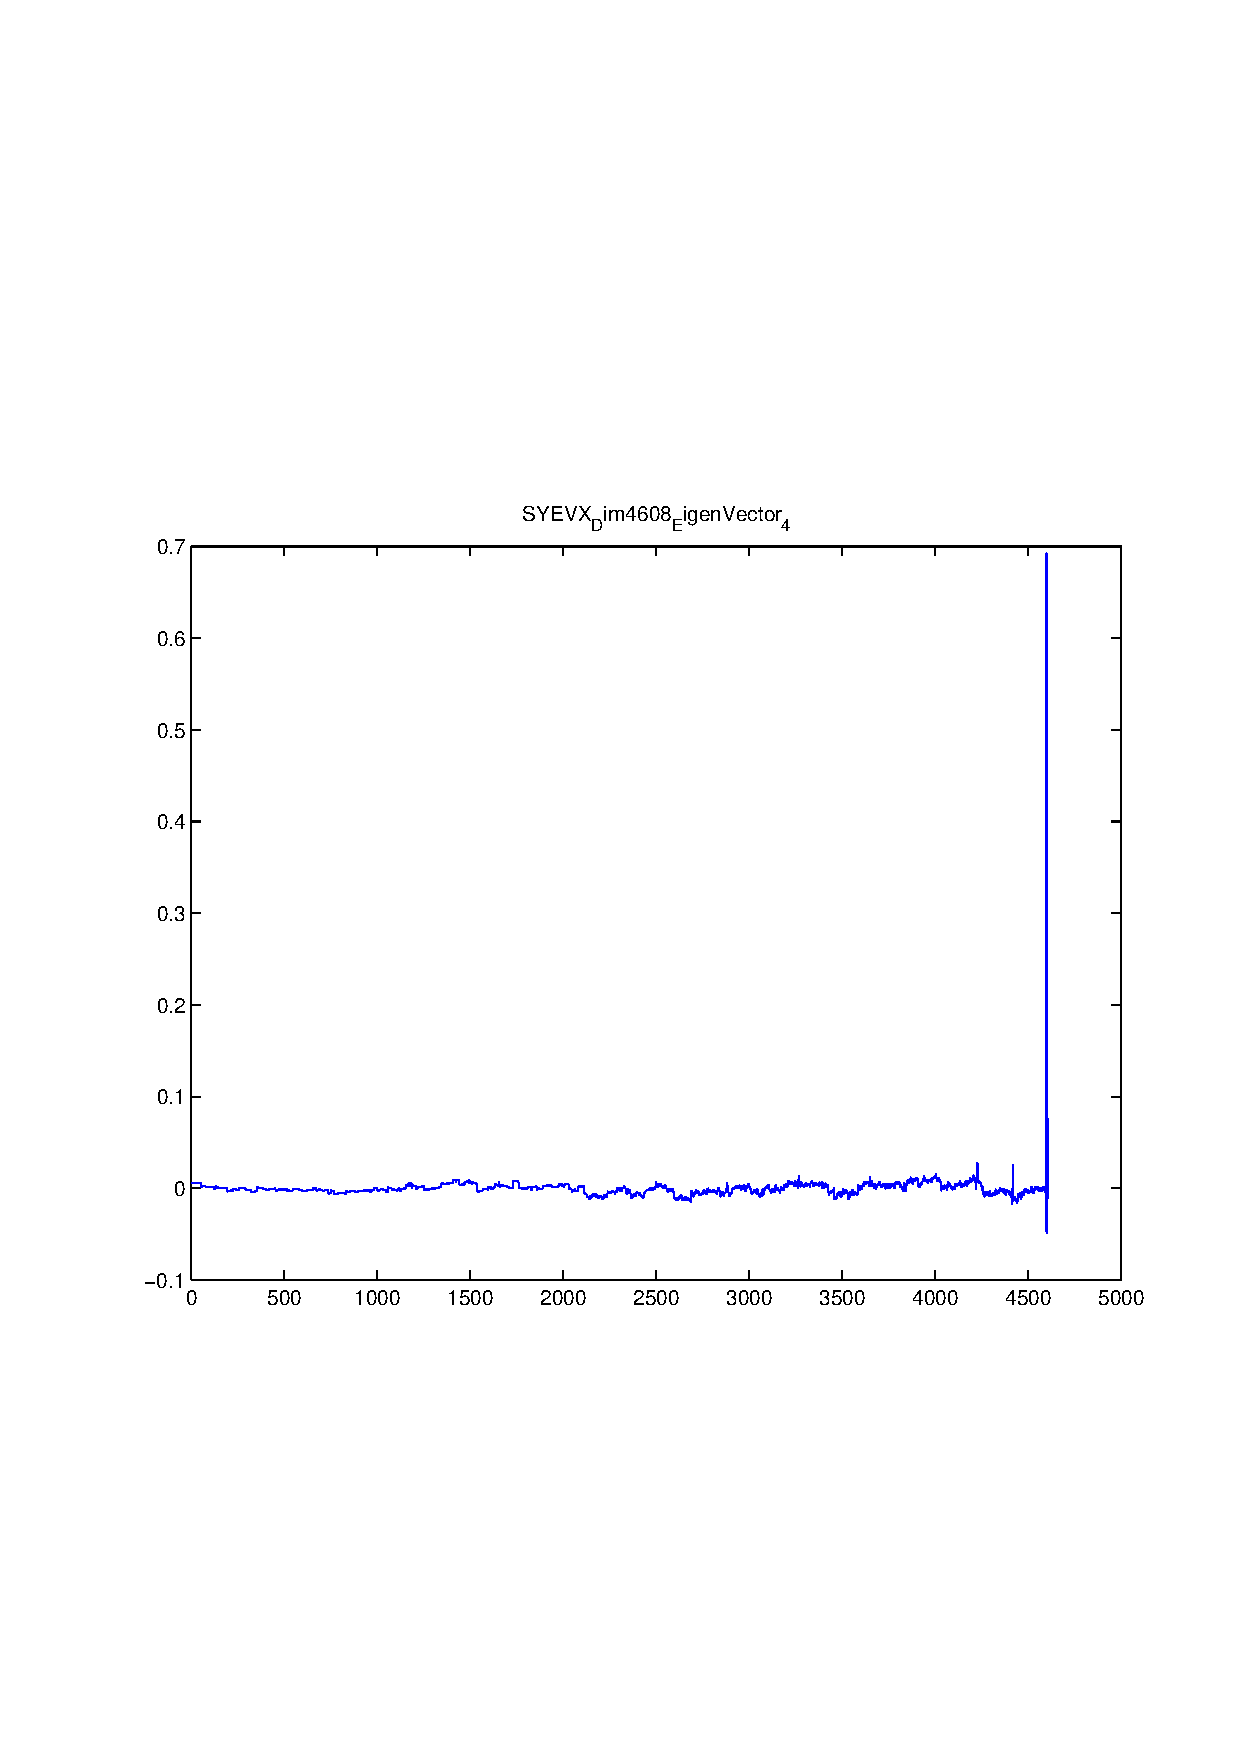
\includegraphics[width=10.0cm,height=10.0cm]{SYEVX_Dim4608_EigenVector_4.pdf}

tic toc fileistream read dim n=5120 dt=155.096
\includegraphics[width=10.0cm,height=10.0cm]{ARPACK_Dim5120_EigenVector_0.pdf}

\includegraphics[width=10.0cm,height=10.0cm]{ARPACK_Dim5120_EigenVector_1.pdf}

\includegraphics[width=10.0cm,height=10.0cm]{ARPACK_Dim5120_EigenVector_2.pdf}

\includegraphics[width=10.0cm,height=10.0cm]{ARPACK_Dim5120_EigenVector_3.pdf}

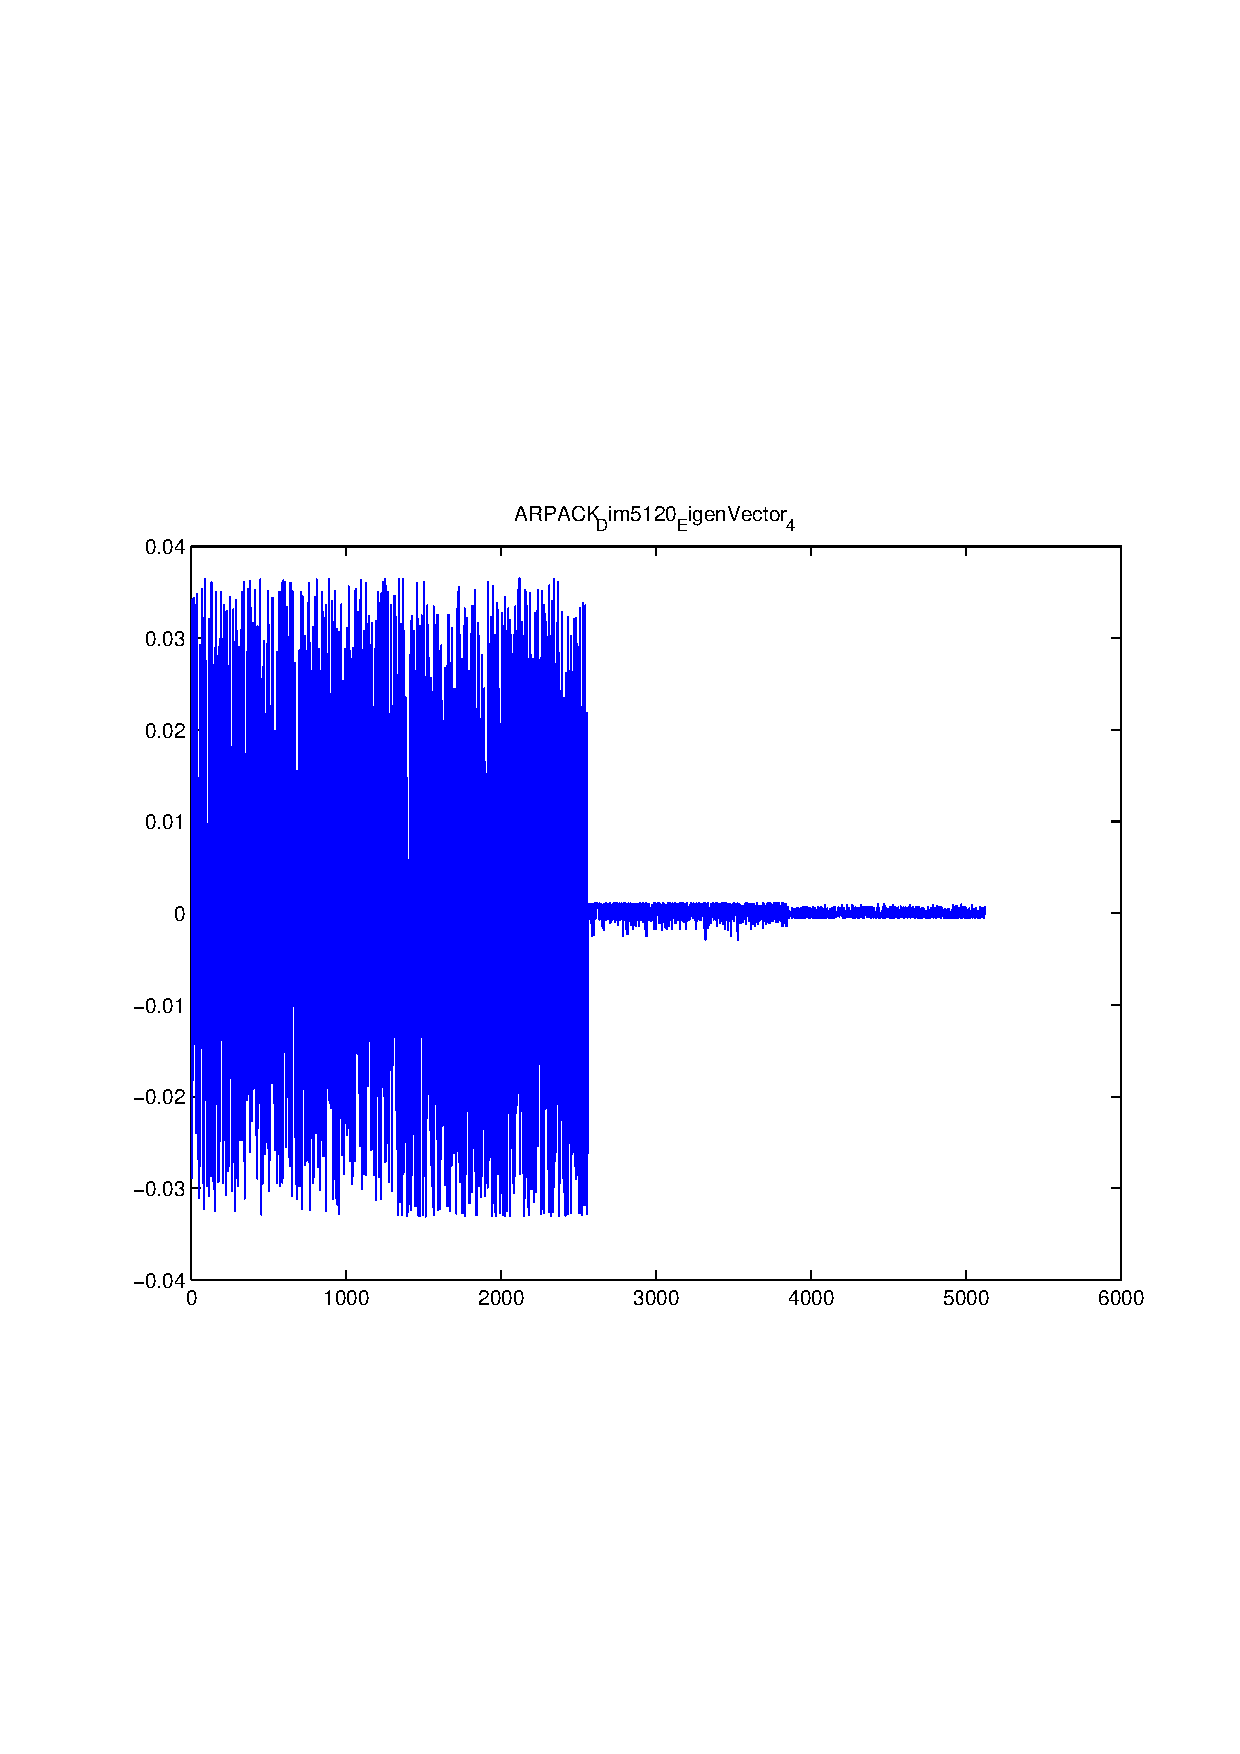
\includegraphics[width=10.0cm,height=10.0cm]{ARPACK_Dim5120_EigenVector_4.pdf}

Iterative Krylov dim=5120 dt=13.0818
\includegraphics[width=10.0cm,height=10.0cm]{SYEVX_Dim5120_EigenVector_1.pdf}

\includegraphics[width=10.0cm,height=10.0cm]{SYEVX_Dim5120_EigenVector_2.pdf}

\includegraphics[width=10.0cm,height=10.0cm]{SYEVX_Dim5120_EigenVector_3.pdf}

\includegraphics[width=10.0cm,height=10.0cm]{SYEVX_Dim5120_EigenVector_4.pdf}

tic toc fileistream read dim n=5632 dt=169.566
\includegraphics[width=10.0cm,height=10.0cm]{ARPACK_Dim5632_EigenVector_0.pdf}

\includegraphics[width=10.0cm,height=10.0cm]{ARPACK_Dim5632_EigenVector_1.pdf}

\includegraphics[width=10.0cm,height=10.0cm]{ARPACK_Dim5632_EigenVector_2.pdf}

\includegraphics[width=10.0cm,height=10.0cm]{ARPACK_Dim5632_EigenVector_3.pdf}

\includegraphics[width=10.0cm,height=10.0cm]{ARPACK_Dim5632_EigenVector_4.pdf}

Iterative Krylov dim=5632 dt=14.7666
\includegraphics[width=10.0cm,height=10.0cm]{SYEVX_Dim5632_EigenVector_1.pdf}

\includegraphics[width=10.0cm,height=10.0cm]{SYEVX_Dim5632_EigenVector_2.pdf}

\includegraphics[width=10.0cm,height=10.0cm]{SYEVX_Dim5632_EigenVector_3.pdf}

\includegraphics[width=10.0cm,height=10.0cm]{SYEVX_Dim5632_EigenVector_4.pdf}

tic toc fileistream read dim n=6144 dt=186.434
\includegraphics[width=10.0cm,height=10.0cm]{ARPACK_Dim6144_EigenVector_0.pdf}

\includegraphics[width=10.0cm,height=10.0cm]{ARPACK_Dim6144_EigenVector_1.pdf}

\includegraphics[width=10.0cm,height=10.0cm]{ARPACK_Dim6144_EigenVector_2.pdf}

\includegraphics[width=10.0cm,height=10.0cm]{ARPACK_Dim6144_EigenVector_3.pdf}

\includegraphics[width=10.0cm,height=10.0cm]{ARPACK_Dim6144_EigenVector_4.pdf}

Iterative Krylov dim=6144 dt=15.6967
\includegraphics[width=10.0cm,height=10.0cm]{SYEVX_Dim6144_EigenVector_1.pdf}

\includegraphics[width=10.0cm,height=10.0cm]{SYEVX_Dim6144_EigenVector_2.pdf}

\includegraphics[width=10.0cm,height=10.0cm]{SYEVX_Dim6144_EigenVector_3.pdf}

\includegraphics[width=10.0cm,height=10.0cm]{SYEVX_Dim6144_EigenVector_4.pdf}

